\documentclass[a4paper,12pt]{article}

\usepackage[left=1.1in,right=1.1in,top=1.2in,bottom=1.2in,
            footskip=.5in]{geometry}

\usepackage[style=apa,sorting=nty]{biblatex}
\addbibresource{references.bib}
\newcommand{\citet}[1]{\textcite{#1}}
\newcommand{\citep}[1]{\parencite{#1}}

\usepackage{appendix}
\usepackage{graphicx}
\usepackage{etoolbox}
\usepackage[font=small]{caption}
\usepackage{tabularx}
\usepackage{booktabs}
\usepackage{setspace}
\onehalfspacing

\usepackage{tikz}
\usetikzlibrary{shapes.geometric, arrows.meta, positioning}
\usepackage{graphicx}

\usepackage{pdflscape}
\usepackage{authblk}
\usepackage{subcaption}
\usepackage{mathtools}
\usepackage{comment}
\usepackage{algorithm}
\usepackage{algpseudocode}
\usepackage{amsfonts}
\usepackage{amsmath}
\usepackage{amssymb}
\usepackage{amsthm}
\DeclareMathOperator*{\argmax}{argmax}
\DeclareMathOperator*{\argmin}{argmin}

\usepackage{xcolor}
\usepackage[colorlinks,citecolor=blue,
  linkcolor=black,
  urlcolor=blue]{hyperref}

\usepackage{enumitem}
\setlist[itemize]{itemsep=-0.5pt}
\setlist[enumerate]{itemsep=-0.5pt}

\setlength{\parindent}{0em}
\setlength{\parskip}{0.7em}

\newtheorem{theorem}{Theorem}[section]
\newtheorem{proposition}[theorem]{Proposition}
\newtheorem{corollary}[theorem]{Corollary}
\newtheorem{assumption}[theorem]{Assumption}
\newtheorem{lemma}[theorem]{Lemma}

\newcommand{\tabitem}{~~\llap{\footnotesize\textbullet}~~}

\newcommand{\todo}[1]{\textcolor{red!80!black}{[\textsc{todo}: #1]}}
\newcommand{\note}[1]{\textcolor{blue!60!black}{\textit{#1}}}

\title{Corporate Omissions:\\[4pt]
Strategic Silence and the Price of Non-Disclosure%
\thanks{Replication code is available at \url{https://github.com/giuliacrippa4/corporate-omissions-article}.
The repository contains the full pipeline -- outcome model, disclosure propensity, exponential tilt,
and every table and figure in the paper. The underlying emissions, accounting and returns data are
licensed from S\&P Trucost, Compustat and CRSP and cannot be redistributed; they must be obtained
from the vendors and placed in the paths documented in the repository.}
}

\author[1]{Giulia Crippa}
\author[2]{Florian Berg}
\author[2]{Roberto Rigobon}
\affil[1]{Princeton University}
\affil[2]{MIT Sloan School of Management}
\date{\today}

\begin{document}

\maketitle

\begin{abstract}
\noindent
Most U.S.\ firms do not disclose their carbon emissions, leaving the samples used to price carbon risk selected on disclosure. We estimate a disclosure equilibrium in which the decision to withhold is driven by latent emissions, and use it to recover the carbon footprints of firms that remain silent. Ignoring this strategic behavior understates aggregate corporate emissions by roughly $12\%$. We then document two additional findings. First, strategic silence is strong where institutional ownership is concentrated, reverses where ownership is dispersed, and appears only among firms with something to hide. Second, the disclosure decision is priced, the emissions level is not: disclosers earn $24$ basis points per month over comparable non-disclosers, orthogonal to the level of recovered emissions.


\vspace{6pt}
\noindent\textbf{Keywords:} voluntary disclosure, carbon premium, selective disclosure, institutional ownership, climate regulation

\noindent\textbf{JEL codes:} G12, G14, Q54, M41, G18.
\end{abstract}

\clearpage

% ============================================================

% \section{Introduction}
% Despite growing standardization efforts, corporate carbon accounting remains fragmented in both coverage and quality. Firms face heterogeneous incentives to disclose their carbon emissions, shaped by regulatory exposure, reputational concerns, and potential financial consequences \citep{christensen2021mandatory}. 


% Most empirical work addressing missing emissions relies on imputation methods that assume data are missing completely at random (MCAR) or missing at random (MAR), implying that the probability of missingness is independent of the unobserved emissions themselves.





% In particular, high-emitting firms may strategically withhold emissions data to avoid scrutiny or adverse stakeholder reactions. Even among disclosers, verification practices vary substantially.


% Accurate measurement of corporate carbon emissions is central to climate policy, sustainable finance, and corporate accountability. As governments, investors, and stakeholders increasingly demand transparency in environmental performance, Scope~1 emissions --  direct greenhouse gas emissions from sources owned or controlled by firms --  have emerged as a foundational metric for assessing corporate contributions to global carbon footprints. Despite growing standardization efforts, corporate carbon accounting remains fragmented in both coverage and quality.

% \clearpage
\section{Introduction}
\label{sec:intro}

Most U.S.\ public firms never disclose their carbon emissions. Pooled over 2012--2023, only about an eighth of firm-years on the major exchanges carry a voluntary Scope~1 figure, and roughly $60\%$ carry no emissions figure of any kind -- not even a data vendor's model-based estimate (Table~\ref{tab:emissions_sources}). The empirical literature on carbon and asset prices is built on the self-selected sample, and it disagrees with itself: \citet{bolton2021investors} find a robust premium in vendor-estimated emissions, \citet{aswani2024carbon} find none in firm-reported emissions, and \citet{pastor2025green} find that whatever premium existed has faded. What the debate has not confronted is that the silent majority is missing for a reason. If a firm withholds its emissions because those emissions are high -- as the classical logic of \citet{grossman1981informational}, \citet{milgrom1981good}, and \citet{verrecchia1983discretionary} implies whenever disclosure is costly -- then every one of these studies conditions on a sample selected on the outcome, and selected in the direction that hides the worst emitters.

That the data are missing not at random is the measurement problem. The economics runs deeper, and it is where the paper aims. Classical disclosure theory attaches to the suspicion discount a condition that is usually stated and rarely tested: silence is informative only if someone is listening. The discount requires an audience that conditions its beliefs on the disclosure decision; where no such audience exists, withholding carries no penalty and the composition of the silent pool need not be adverse at all. The theory therefore predicts not merely \emph{that} strategic silence occurs but \emph{where}, and the sign of selection is the observable that separates the two regimes. Testing this needs two things that rarely coexist: a measure of what silent firms withheld, and variation in the audience that is uncorrelated with the quantity being hidden. Corporate carbon disclosure supplies both -- emissions are physically determined by scale and technology, so what a silent firm hides can be recovered from firms that disclose, and institutional ownership varies sharply across firms whose production technology is otherwise identical. Ownership is of course correlated with size, liquidity and the capacity to measure one's own emissions, and any of those would produce a gradient in selection with no audience doing the work. But the correlates predict a gradient uniformly, whereas an audience can only penalize silence that conceals something. The two accounts are therefore separated not by the ownership gradient itself but by whether it survives where there is nothing to hide.

We formalize the mechanism in a disclosure game with a cost of revelation that rises in the emissions revealed. In our model, the equilibrium disclosure rule is logistic in firm characteristics and latent emissions, and its slope on emissions is a single index, $\gamma$ -- the \emph{selection severity index} -- that measures the strength of missing-not-at-random selection. The index decomposes additively as $\gamma=(\beta+c_1)/\lambda$, with $\beta$ the market's price impact on revealed emissions and $c_1$ the private cost of revelation, so anything that raises regulatory or investor scrutiny raises it. Adding a transparency benefit that accrues only where an audience rewards revealed commitment yields an effective severity that changes sign as the benefit crosses the cost: the audience condition of \citet{milgrom1981good} and \citet{verrecchia1983discretionary} becomes a sign restriction on an estimable parameter. The missing-data structure and the exponential-tilting correction we use to undo it both emerge as equilibrium objects rather than statistical assumptions.

Estimating $\gamma$ requires emissions for firms that did not disclose, which is the measurement problem solved as a by-product. In equilibrium the emissions density of silent firms is a one-parameter exponential tilt of the disclosed density with tilt parameter $\gamma$ \citep{kim2011semiparametric}, so recovery reduces to estimating $\gamma$ and applying the tilt. Identification uses a shifter of emissions excluded from the disclosure decision \citep{wang2014instrumental}: we interact the crude-oil price with each firm's predetermined physical-capital intensity \citep{goldsmithpinkham2020bartik}, so that identification comes from the difference, within a year and sector, between the disclosure choices of more and less oil-exposed firms. This delivers a Scope~1 figure for the full Compustat universe of major-exchange firms -- including the never-disclosing majority, on whom prior work is silent. Relative to a missing-at-random baseline the correction adds mass to the upper tail and raises aggregate Scope~1 emissions by 12\%; valued at the social cost of carbon, the recovered universe carries corporate carbon damages more than twice the \citet{greenstone2023mandatory} benchmark for the S\&P~1500, a gap concentrated in the smaller, carbon-intensive firms that disclose least. Among the firms that later begin disclosing, the recovered value is nearly unbiased in the upper tail, where vendor estimates understate by roughly half.

The sharpest result is that the sign of selection tracks the audience, on two margins. In the cross-section, we sort firms into institutional-ownership terciles \emph{within} sector -- holding production technology fixed while moving only the presence of monitoring investors. Strategic silence is strong where ownership is concentrated ($\hat\gamma=+0.162^{***}$ in the top tercile) and weakens to zero or below where it is dispersed; the top-minus-bottom difference is $+0.226$ ($p<0.001$). That gradient is not firm sophistication in disguise, because it appears only where silence has something to conceal. Splitting the same firms a second time by the carbon intensity of their industry -- computed from disclosing firms alone, so that no imputed value enters the split -- the ownership gradient is $+0.225$ ($p<0.001$) among high-emitting firms and $-0.147$ ($p=0.007$) among clean ones, a triple difference of $+0.372$ ($p<0.001$). Size, liquidity and reporting capacity predict a gradient of the same sign in both halves; only an audience that reads silence as bad news predicts one that vanishes where there is no bad news to read. Over time, $\hat\gamma_t$ is statistically indistinguishable from zero through 2020 and then rises to $+0.14^{***}$, $+0.20^{***}$, and $+0.22^{***}$ in 2021--2023 -- the period coinciding with the surge in sustainable investment and the build-up to the SEC's proposed climate-disclosure rule. 

With emissions recovered for every firm, we can finally separate the two objects the disclosing-sample literature could only observe jointly: the pricing of the emissions \emph{level} and the pricing of the disclosure \emph{decision}. The decision is what carries a premium. Voluntary disclosers earn $0.242^{***}$ percentage points per month more than observably comparable silent firms, orthogonal to the emissions level, which enters at zero. We read this as a cross-sectional differential tied to the characteristics of firms that disclose rather than a causal return to the act -- within a firm, the transition into disclosure if anything lowers returns. The level of emissions itself is not priced: it is flat among disclosers, and what robust loading the emissions data carry attaches to \emph{intensity}, is negative, and reads as the realized green outperformance of \citet{pastor2025green} rather than a risk premium.

Through the model these results cohere. The transition to disclosure return is $-\beta\,(y-\mu_{ND})$, so the common message of the pricing tests is that $\beta$, the market's price impact on revealed emissions, is small in this sample; and with $\beta$ small, the selection severity of Section~\ref{sec:mechanism} -- and its intensification over 2021--2023 -- is essentially the $c_1$ channel, the private and regulatory cost of revelation rather than a standing carbon-risk premium. The two-channel decomposition survives, and the data tell us which channel is operative.

The paper contributes to three literatures. To voluntary-disclosure theory \citep{grossman1981informational,milgrom1981good,verrecchia1983discretionary,dye1985disclosure}, it provides the first direct test of \emph{where} the strategic-silence mechanism operates, by making the sign of selection an estimable prediction, confirming it across audiences, and separating the audience from the firm characteristics it travels with. To the missing-data and ESG-measurement literatures \citep{kim2011semiparametric,wang2014instrumental,yang2017semiparametric,olesiewicz2021navigating,chen2025green,duan2025imputation}, it derives the missing-not-at-random mechanism and its correction as equilibrium objects rather than imposing them, and shows that the corrected measure delivers cleaner asset-pricing identification than vendor estimates. To the carbon asset-pricing literature \citep{bolton2021investors,aswani2024carbon,pastor2025green}, it extends the sample from the self-selected disclosing subset to the full public universe and locates the priced object in the disclosure decision rather than the emissions level. 

The paper proceeds as follows. Section~\ref{sec:theory} develops the disclosure-equilibrium model and derives $\gamma$, the exponential tilt, and the sign prediction; Section~\ref{sec:data} describes the data. Section~\ref{sec:measurement} estimates $\gamma$, recovers the missing cross-section, and reports the aggregate-emissions and carbon-damage implications. Section~\ref{sec:mechanism} locates strategic silence -- the ownership cross-section and the brownness interaction that establish where it operates, and the rising selection severity that dates when its audience formed. Section~\ref{sec:pricing} contains the pricing tests: the transparency premium, the within-firm transition that qualifies it, and the market reaction to the SEC's proposed mandate. Section~\ref{sec:conclusion} concludes.




% ============================================================
% \section{Related Literature}
% \label{sec:lit}

% \paragraph{Voluntary disclosure theory.}
% The foundations of this paper lie in the classical theory of voluntary disclosure. \citet{grossman1981informational} and \citet{milgrom1981good} establish the unraveling result: when disclosure is costless and verifiable, rational observers infer the worst from silence and full disclosure obtains in equilibrium. \citet{verrecchia1983discretionary} and \citet{dye1985disclosure} relax the unraveling logic by introducing positive disclosure costs, generating partial-disclosure equilibria with threshold disclosure rules. Our model extends this tradition by making the disclosure cost linear in the magnitude of the privately-observed signal --  emissions. This generates a logistic equilibrium propensity in which the strength of MNAR selection is governed by a single structural parameter $\gamma$, rather than a binary threshold rule, and provides a structural microfoundation for the exponential tilting correction of \citet{kim2011semiparametric}.

% \paragraph{Carbon risk and asset pricing.}
% A growing literature studies whether carbon-intensive firms earn a risk premium in equity markets. \citet{bolton2021investors} document a robust positive premium using emissions data inclusive of Trucost vendor estimates. \citet{aswani2024carbon} find no such premium when emissions are restricted to firm-reported values. \citet{pastor2025green} document attenuation of the premium over the recent sample. All three studies share a maintained sample restriction --  attention is limited to firms with some emissions coverage, whether disclosed or vendor-estimated. We extend the relevant population to the full universe of U.S.\ public firms, including the substantial majority absent from vendor coverage entirely, and identify the disclosure decision itself as a priced signal that is orthogonal to the level of disclosed emissions.

% \paragraph{Missing data under non-ignorable selection.}
% We build on the missing-data taxonomy of \citet{little1988test} and \citet{rubin1987statistical} and on the identification results of \citet{wang2014instrumental} for MNAR settings via excluded shifters. The exponential-tilting representation we adopt follows \citet{kim2011semiparametric} and is extended semiparametrically by \citet{yang2017semiparametric}. Our contribution to this literature is to derive the MNAR structure and the tilting correction as equilibrium objects in a disclosure game, rather than imposing them as modeling assumptions.

% \paragraph{Concurrent work.}
% \citet{chen2025green} develop a double machine learning estimator for the carbon premium under a missing-at-random assumption conditional on observables. \citet{duan2025imputation} provide imputation-powered inference under the same boundary condition. Both approaches do not model the selection process and therefore inherit MAR; our framework is complementary in modeling the disclosure decision explicitly. \citet{olesiewicz2021navigating} is the closest ML application of MNAR in the carbon-disclosure setting; we add a game-theoretic microfoundation, IV-based identification, and the asset-pricing application.

% \paragraph{Corporate disclosure and climate accounting.}
% \citet{christensen2021mandatory} and \citet{berg2024importance} study the effects of mandatory disclosure regimes and third-party assurance on the reliability of corporate emissions reporting. \citet{greenstone2023mandatory} develop a corporate carbon damages framework based on the social cost of carbon, which we apply to our MNAR-corrected aggregate emissions in Section~\ref{sec:aggregate}. \citet{cheema2021decarbonizing} document measurement heterogeneity and double-counting risks in Scope~2 and Scope~3 reporting that motivate our focus on Scope~1.

% ============================================================

\section{Theoretical Framework}
\label{sec:theory}

This section develops a game-theoretic model of voluntary emissions disclosure. We begin by locating the model within the classical theory of disclosure, which supplies both the economic logic --  silence is informative --  and the specific frictions that allow non-disclosure to survive in equilibrium. We then specify the primitives, derive the equilibrium disclosure rule and the selection severity index $\gamma$, translate the equilibrium into an estimable correction for the missing emissions distribution, and characterize how $\gamma$ responds to regulatory and market forces.

\subsection{Voluntary disclosure and the informativeness of silence}
\label{subsec:disclosure_theory}

The economics of voluntary disclosure\footnote{For surveys, see \citet{verrecchia2001essays} and \citet{beyer2010financial}.} begins with a striking benchmark. When a privately-informed party can disclose its information at no cost, and disclosures are \emph{verifiable} --  the firm may withhold but cannot fabricate --  then no information is withheld in equilibrium. The argument is the \emph{unraveling} logic of \citet{grossman1980disclosure}, \citet{grossman1981informational} and \citet{milgrom1981good}. A firm holding the most favorable news discloses to separate itself from the pool; its departure lowers the market's expectation of the firms that remain silent; the best of the remaining firms then finds it optimal to disclose in turn; and the iteration continues until only the single worst type is left withholding. Rational skepticism about silence --  the market assumes the worst about anything not revealed --  forces full revelation. In this frictionless benchmark there is no missing data to speak of: the very possibility of concealment is undone by the inference it invites.

Systematic non-disclosure therefore has to be explained by a departure from this benchmark, and the literature offers two canonical models. The first introduces a \emph{positive disclosure cost}. \citet{verrecchia1983discretionary} shows that when revealing information is costly, unraveling halts at an interior threshold: firms whose news is favorable enough to justify the cost disclose, while those below the threshold pool in silence. The withholding region is no longer a single worst type but a whole interval, and its size grows with the cost. The second departure introduces \emph{uncertainty about whether the firm is informed}. \citet{dye1985disclosure} and \citet{jung1988disclosure} observes that if the market cannot tell an uninformed firm (which has nothing to disclose) from an informed firm that is concealing bad news, then silence is no longer unambiguous proof of bad news, and informed firms can hide behind the uninformed. Both frictions break full unraveling and, crucially for our purposes, generate an equilibrium in which a systematic, non-random subset of firms is silent.

What unifies these models, and what we carry into the carbon setting, is that \emph{silence is priced}. A firm that does not disclose is not treated as an average firm; it is priced at the conditional expectation of the withholding pool, which under adverse selection lies strictly below the unconditional mean. This ``suspicion discount'' is the economic content of non-disclosure: the market's rational conjecture about what is being hidden, applied uniformly to everyone who hides it. In the emissions context the mapping is immediate. The private signal is the firm's Scope~1 emissions; ``bad news'' is high emissions; and the cost of disclosure --  regulatory scrutiny, litigation exposure, and reputational damage --  plausibly scales with the quantity revealed. A firm that stays silent about its carbon footprint is pooled with, and priced like, the other silent firms, which are disproportionately high emitters.

Two modeling choices turn this qualitative logic into an estimable object. First, we make the disclosure cost increase in the \emph{magnitude} of emissions rather than imposing a fixed cost. This replaces the binary threshold rule of \citet{verrecchia1983discretionary} and \citet{dye1985disclosure} with a smooth disclosure propensity that is logistic in latent emissions and is indexed by a single structural parameter, $\gamma$ --  the \emph{selection severity index}. In the language of the missing-data taxonomy \citep{little2019statistical}, strategic withholding is exactly a \emph{missing-not-at-random} (MNAR) mechanism: the probability that an emissions value is unobserved depends on that very value. This is precisely the case ruled out by the missing-at-random (MAR) assumption on which conventional imputation relies, and it is the source of the bias we correct. Second, as we show below, the density of emissions among silent firms is a one-parameter exponential tilt of the disclosed density, with tilt parameter $\gamma$ \citep{kim2011semiparametric}. The correction that undoes selection is thus fully summarized by the same $\gamma$ that governs the disclosure decision --  an equilibrium implication of the model, not an assumption imposed on the data.

Finally, the theory is explicit about a boundary condition that our empirical design exploits. Silence is informative only when someone \emph{interprets} it: the suspicion discount requires an audience that conditions its beliefs on the disclosure decision. Where no such audience exists --  where carbon carries little regulatory or investor scrutiny --  adverse inference has no bite, and the disclosure decision is governed instead by motives such as signaling to attract capital or idiosyncratic owner preferences, under which the sign of selection can reverse. The model therefore predicts not merely \emph{that} MNAR selection exists but \emph{where}: $\gamma > 0$ in environments with an interpreting audience, and $\gamma \leq 0$ where that audience is absent. This sign prediction across observable environments is the theory's empirical fingerprint, and it is what makes the Milgrom-- Verrecchia mechanism testable rather than merely invoked.

\subsection{Primitives}
\label{subsec:primitives}

Consider a unit continuum of firms $i \in [0,1]$. Firm $i$ privately assesses its Scope 1 emissions $y_i \in \mathbb{R}$, with market prior $y_i \sim \mathcal{N}(y_0, h_0^{-1})$; let $\phi$ denote the prior's density.\footnote{We write ``assesses'' rather than ``observes'' deliberately. Producing a \emph{verifiable} emissions figure requires measurement and, often, third-party assurance -- this is the costly act the firm chooses over -- whereas forming an internal assessment of whether one is a high- or low-emission firm, from directly-observed fuel and energy use, is comparatively cheap. It is this decision-relevant assessment, not an audited number, that the firm brings to the disclosure choice. Firms lacking even the internal assessment -- the uninformed type of \citet{dye1985disclosure} -- are treated in the remark following Corollary \ref{cor:expo_tilt}.} Let $x_i  \in \mathbb{R}^k$ denote firm's $i$ observable characteristics. The firm chooses $\delta_i \in \{0,1\}$ (disclose/withhold) to maximize price net of disclosure costs. We work with $y_i$ in logs throughout, so that ``high emissions'' refers to the upper tail of the log distribution and the Gaussian prior is the empirically relevant benchmark for the outcome model of Section~\ref{sec:methodology}.

\paragraph{Timing and information.} The disclosure game unfolds over three dates. At $t=0$, nature draws each firm's emissions $y_i$ from the prior and an idiosyncratic disclosure-cost shock $\tilde\eta_i$; the firm privately learns its own type -- its emissions assessment $y_i$ and its cost shock $\tilde\eta_i$ -- while the market observes only the characteristics $x_i$ and the common prior. At $t=1$, firms simultaneously choose $\delta_i \in \{0,1\}$. At $t=2$, the market observes the disclosure profile, forms its posterior information set $\Omega$, and prices each firm through the schedule below. Two features of this environment do the work in what follows. First, disclosure is \emph{verifiable}: a firm that discloses reveals its true $y_i$ and cannot misreport, so the only strategic margin is whether to reveal at all, exactly as in the \citet{grossman1981informational}-- \citet{milgrom1981good} tradition. Second, because firms form a continuum, no individual firm's report moves the composition of the non-disclosure pool; the pricing of silence is therefore a fixed point of the market's beliefs rather than a bilateral inference, which is what renders the equilibrium tractable.

We adopt the following price function\footnote{Note that, we depart from the canonical \citet{verrecchia1983discretionary} variance-discount price $P(\Omega) = \mathbb{E}[y \, \mid \Omega] - \rho \, \textrm{Var}[y \, \mid \Omega]$ under the assumption that the penalty for silence is purely driven by adverse inference --  the silent firm is priced at the pooling mean of non-disclosers in the tradition of \citet{milgrom1981good} and \citet{dye1985disclosure} --  rather than uncertainty aversion.}, 

\begin{equation}
\label{eq:price}
    P(\Omega) = V_0 - \beta \, \mathbb{E}[y \, \mid \Omega], \qquad \beta > 0, 
\end{equation}

where $\Omega$ is the market's information set after observing $\delta_i$, $V_0$ is a baseline value, and $\beta$ is the equilibrium price impact per unit of revealed emissions, i.e. the carbon-risk premium of \citet{bolton2021investors} and \citet{pastor2025green} and it operates through revelation. When $\delta_i = 1$, then a disclosing firm is priced at its revealed emissions level $y_i$; when $\delta = 0$, a silent firm is priced at the market's rational expectation over the non-disclosing pool. In particular, the value of silence equals $V_0 - \beta \, \mathbb{E}[y \, \mid \delta = 0]$. 

\subsection{The selection severity index}
\label{subsec:severity}

The price schedule \eqref{eq:price} is the \emph{benefit} side of the disclosure decision: revealing $y_i$ moves the firm off the pooling price of silence and onto its own price -- attractive for a low emitter, punishing for a high one. What disciplines the decision is the \emph{cost} of coming forward, which we now specify. The central modeling choice, and the point of departure from the threshold models of \citet{verrecchia1983discretionary} and \citet{dye1985disclosure}, is that this cost rises with the \emph{magnitude} of emissions the firm would have to report: regulatory scrutiny, litigation exposure, and reputational damage all scale with how much carbon a disclosure reveals, so a high emitter pays more to disclose than a low emitter does. This single feature is what will make selection non-ignorable. Formally, disclosure is costly,

\begin{equation}
\label{eq:cost}
    \tilde{c_i} = c_0(x_i) + c_1 y_i + \lambda \tilde{\eta_i}, \qquad c_0, c_1, \lambda >0, 
\end{equation}

where $c_0(x_i)$ is a fixed cost, $c_1$ is the per-unit cost of disclosing emissions, and $\tilde{\eta_i}$ a mean-zero idiosyncratic shock. The emissions dependent term $c_1 y_i$ is the engine of MNAR selection, and extends the proprietary-cost mechanism of \citet{verrecchia1983discretionary} and \cite{dye1985disclosure}, in which firms with sufficiently unfavorable private information withhold. The fixed cost $c_0(x_i)$ absorbs firm- and sector-level determinants of disclosure -- measurement infrastructure, board and investor pressure, prevailing reporting norms -- while $c_1$ isolates the marginal deterrent specific to the emissions level, the object our identification targets.

To turn this benefit-- cost trade-off into a sharp disclosure rule, we impose a standard distributional structure on the idiosyncratic component.

\begin{assumption}
\label{ass:logistic_shocks}
    The shocks $\tilde{\eta_i}$ are i.i.d. standard logistic and independent of $y_i$ and $x_i$. 
\end{assumption}

Assumption \ref{ass:logistic_shocks} relies on the discrete-choice tradition of \citet{mcfadden1972conditional}. The logistic form is what delivers the closed-form exponential tilt of Corollary~\ref{cor:expo_tilt}: the odds ratio $(1-\Lambda)/\Lambda = e^{-z}$ is exactly log-linear, so the density ratio $f_0/f_1$ is exactly $e^{\gamma y}$. The qualitative structure, however, does not depend on it. For any shock density that is log-concave with full support, the disclosure rule remains a monotone threshold in $y$, so higher emitters disclose less whenever $\gamma>0$ and the sign and monotonicity of the selection bias in Proposition~\ref{prop:mnar_bias} are preserved; only the functional form of the tilt changes, from exponential to the density-specific ratio. We adopt the logistic throughout for the closed form it affords.

\begin{lemma}[Individual best response]
\label{lemma:indiv_best_resp} Fix the non-disclosure firms mean $\mu_{ND} = \mathbb{E}[y \, \mid \delta = 0]$. Under \eqref{eq:price}, \eqref{eq:cost} and Assumption \ref{ass:logistic_shocks}, firm $i$ discloses iff 
\begin{equation}
\label{eq:disclosure_threshold}
    \tilde{\eta_i} \leq f(x_i) - \gamma \, y_i, \qquad f(x_i) \equiv \frac{1}{\lambda}[\beta \, \mu_{ND} - c_0(x_i)], \qquad \gamma \equiv \frac{\beta + c_1}{\lambda} > 0, 
\end{equation}
so the conditional disclosure propensity is $\mathbb{P}(\delta_i \mid \, x_i, y_i) = \Lambda(f(x_i) - \gamma y_i)$, where $\Lambda$ is the CDF of a standard logistic. 
\end{lemma}

\textit{Proof.} See Appendix~\ref{app:proofs}. \hfill $\square$


Lemma \ref{lemma:indiv_best_resp} takes the pooling mean $\mu_{ND}$ as given. But $\mu_{ND}$ is itself an equilibrium object: the disclosure rule determines which firms stay silent, which determines the mean of the silent pool, which feeds back into the threshold $f(x_i)$ through the value of silence. Closing the model requires a $\mu_{ND}$ consistent with the disclosure behavior it induces. Theorem \ref{thm:existence} establishes that such a fixed point exists and is unique, and -- crucially -- that the emissions slope $\gamma$ is pinned down independently of it.

\begin{theorem}[Existence, uniqueness, logistic propensity] \label{thm:existence}
Under \eqref{eq:price}-\eqref{eq:cost}, Assumption \ref{ass:logistic_shocks}, and regularity, there exists a unique equilibrium threshold $f^*$, and the equilibrium disclosure propensity is 
\begin{equation}
\label{eq:threshold}
\mathbb{P}(\delta_i \mid \, x_i, y_i) = \Lambda(  f^* - \gamma y_i), \qquad \gamma = \frac{\beta + c_1}{\lambda} > 0. 
\end{equation}

\end{theorem}
\textit{Proof.} See Appendix~\ref{app:proofs}. \hfill $\square$

\textit{Remark}. $\gamma$ is fixed by the slope of the disclosure inequality and is invariant to the continuum assumption and the existence/uniqueness of $f^*$. Multiplicity of $f^*$, were it to arise, would relocate the threshold but leave the identified $\gamma$ unchanged.

The two components of the equilibrium propensity play distinct roles. The intercept $f^*$ absorbs everything that shifts the disclosure decision uniformly across emission levels -- the fixed cost $c_0(x_i)$, the pooling value of silence, and any characteristic in $x_i$ -- and is a nuisance object for our purposes. The slope $\gamma$ is the parameter of interest: it measures how sharply the disclosure probability falls as latent emissions rise, and it is the sole channel through which the \emph{level} of emissions enters the decision. Its structure, $\gamma = (\beta + c_1)/\lambda$, shows that a single index aggregates two economically distinct forces -- the market's carbon-risk price $\beta$ and the private per-unit cost of revelation $c_1$ -- each normalized by the dispersion $\lambda$ of the idiosyncratic shock. This is what makes $\gamma$ a \emph{sufficient statistic} for selection: two economies with different primitives but the same $(\beta + c_1)/\lambda$ generate identical disclosure patterns and identical MNAR bias. The empirical program of the paper is, in effect, the estimation of this one index and the interpretation of its variation across environments and over time.

\subsection{From equilibrium to empirical correction}
\label{subsec:correction}

The equilibrium in Theorem \ref{thm:existence} is a statement about disclosure \emph{propensities}. To take the model to data on emissions, we need the object it implies for the \emph{distribution} of the values that go unobserved. The next result supplies it: the density of emissions among silent firms is a one-parameter exponential tilt of the disclosed density, governed by the same $\gamma$. This is the bridge from equilibrium to estimation -- it shows that the entire correction for non-ignorable selection is summarized by the selection severity index, which the propensity model of Section~\ref{sec:methodology} identifies, so that no separate assumption on the missing-data mechanism is required.

\begin{corollary}[Exponential Tilting] \label{cor:expo_tilt} Let $f_1(y \mid x)$ and $f_0(y \mid x)$ denote the conditional emission densities for disclosing and non-disclosing firms, respectively. Under \eqref{eq:threshold}, 

\begin{equation}
\label{eq:tilting}
    f_0(y \mid x) = f_1(y \mid x) \cdot \dfrac{\exp{\gamma y}}{\mathbb{E}[\exp{\gamma \tilde{y}} \, \mid x, \delta =1 ]}.
\end{equation}
\end{corollary}

\textit{Proof.} See Appendix~\ref{app:proofs}. \hfill $\square$

Equation~\eqref{eq:tilting} is the exponential-tilting representation of \citet{kim2011semiparametric}, extended semiparametrically by \citet{yang2017semiparametric}; here it is derived as an equilibrium consequence rather than posited as a missing-data assumption. It applies without a mixture correction whenever every non-discloser holds the internal assessment on which the disclosure rule acts, so that silence is always a strategic choice; the remark below relaxes this and shows the relaxation reproduces exactly the missing-at-random baseline that the empirical procedure already imposes.

\textbf{Remark} (Uninformed firms and the MAR component). Corollary \ref{cor:expo_tilt} treats every non-discloser as a strategic withholder. Some firms plausibly lack even the internal assessment -- they have never measured their emissions and thus cannot produce a verifiable disclosure regardless of $y_i$, the uninformed type of \citet{dye1985disclosure} and \citet{jung1988disclosure}. Let a firm be informed with probability $\rho(x_i)$ that, conditional on $x_i$, is independent of $y_i$. Non-disclosure then pools two populations, and the silent-firm density is the mixture
\begin{equation}
\label{eq:tilting_mixture}
    f_0(y \mid x) \ \propto\ \underbrace{\big(1-\rho(x)\big)\, f(y \mid x)}_{\text{uninformed: MAR}}\ +\ \underbrace{\rho(x)\,\big(1 - \Lambda(f^* - \gamma y)\big)\, f(y \mid x)}_{\text{strategic: MNAR tilt}},
\end{equation}
whose first term is the unconditional (missing-at-random) density of the uninformed and whose second is the exponential tilt \eqref{eq:tilting} of the strategic withholders. This is the structure the empirical procedure imposes: the baseline MAR imputation of Section~\ref{sec:methodology} recovers the first term and the exponential-tilt reweighting recovers the second. The pure tilt \eqref{eq:tilting} is the $\rho \equiv 1$ special case; because $\rho$ is conditioned on $x$ but not $y$, the uninformed margin is ignorable and $\hat\gamma$ retains its interpretation as the strength of \emph{strategic} selection.

Corollary~\ref{cor:expo_tilt} pins down the full \emph{shape} of the correction, the entire density of unobserved emissions. For most purposes, though, what matters is a single summary of it: how far, and in which direction, selection moves the average silent firm away from the average discloser. This is the object a researcher who observes only disclosers gets wrong, and the next result characterizes it. It shows the gap has a definite sign and grows monotonically in the selection severity, so that $\gamma$ orders economies not only by how they select but by how badly a naive disclosed-sample comparison understates the rest.

\begin{proposition}[Monotone MNAR bias] \label{prop:mnar_bias}
Define $\Delta \mu(\gamma) \equiv \mathbb{E}[y|\delta =0] - \mathbb{E}[y|\delta =1]$. Under \eqref{eq:threshold}, $\Delta \mu(0) = 0$, $\Delta \mu(\gamma) > 0$ for all $\gamma > 0$, and $\Delta \mu$ is strictly increasing in $\gamma$. 
\end{proposition}

\textit{Proof.} See Appendix~\ref{app:proofs}. \hfill $\square$

Proposition \ref{prop:mnar_bias} is the equilibrium analog of the upward revision in reported emissions that follows mandatory-disclosure mandates \citep{christensen2021mandatory}: the average non-discloser is a higher emitter than the average discloser whenever strategic silence operates.

The result is sharp about \emph{how} that gap grows. As the proof shows, the marginal effect of selection is $d\Delta\mu/d\gamma = \mathrm{Var}_\gamma[y]$, the variance of emissions within the silent pool: selection bites harder precisely where the emissions distribution is more dispersed, because a steeper tilt then has more upper-tail mass to redistribute. When the disclosing-firm density is approximately Gaussian with variance $\sigma_1^2$, the relationship collapses to the closed form
\begin{equation}
\label{eq:gaussian_bias}
    \Delta\mu(\gamma) = \gamma\,\sigma_1^2,
\end{equation}
so the mean of the silent pool exceeds that of disclosers by exactly the selection severity scaled by the dispersion of disclosed emissions. The bias is not an artifact of functional form; it is a direct, monotone reading of $\gamma$, and it vanishes only in the knife-edge case $\gamma = 0$.

That knife-edge is exactly the missing-at-random benchmark. At $\gamma = 0$, silence carries no information about $y$: disclosing and non-disclosing firms are drawn from the same conditional distribution, and any imputation that ignores selection is unbiased. For every $\gamma > 0$, by contrast, a firm's silence is itself evidence that it sits higher in the emissions distribution, so conventional MAR imputation \emph{understates} the emissions of non-disclosers -- and understates them more, the larger is $\gamma$. This is the theoretical content behind the aggregate correction we report in Section~\ref{sec:measurement}: because the overwhelming majority of firms are silent, even a moderate $\hat\gamma$ compounds into a substantial upward revision of aggregate emissions relative to the MAR baseline. Proposition~\ref{prop:mnar_bias} guarantees that this revision is signed and monotone, so its entire magnitude is governed by the single index the propensity model estimates -- which is what makes the question of the next subsection, what moves $\gamma$, the economically decisive one.

\subsection{Time variation and the regulatory channel}
\label{subsec:timevariation}

Because the selection severity index is a function of the structural primitives, $\gamma = (\beta + c_1)/\lambda$, anything that shifts those primitives shifts the observable strength of selection. This is what allows us to read regulatory and market forces directly off the estimated $\hat\gamma$ -- across sectors and ownership structures in the cross-section, and across time as scrutiny intensifies, among the others. The two results below make the comparative statics precise and then show how an audience-dependent benefit can flip the sign of $\gamma$, delivering the boundary condition previewed in Section~\ref{subsec:disclosure_theory}.

\begin{proposition}[Regulatory and market-sensitivity channels] \label{prop:regulatory_channel}
Under \eqref{eq:threshold},

\begin{equation}
    \frac{\partial \gamma}{\partial c_1} = \frac{1}{\lambda} >0, \qquad  \frac{\partial \gamma}{\partial \beta} = \frac{1}{\lambda} >0, \qquad  \frac{\partial \gamma}{\partial \lambda} = - \frac{\beta + c_1}{\lambda^2} <0.
\end{equation}
\end{proposition}

\textit{Proof}. Immediate from $\gamma = (\beta + c_1)/\lambda$, treating $\beta, \, c_1, \, \lambda$ as structural primitives. \hfill \qed

A rise in the per-unit disclosure cost $c_1$ (tighter regulatory scrutiny or litigation exposure) or in the revealed-emissions price impact $\beta$ (stronger carbon-risk pricing by ESG-aware investors) raises the selection severity index $\gamma$, additively and symmetrically. The empirical analog is an intensification of $\hat{\gamma}_t$ when regulatory salience or investor attention to carbon risk rises. The baseline yields $\gamma >0$ for all primitives. Empirically observed reverse selection $\hat{\gamma}<0$ in low-attention contexts requires a counter-force. The following extension generates it endogenously and delivers the audience boundary condition that is the empirical fingerprint of the \citet{milgrom1981good}-- \citet{verrecchia1983discretionary} mechanism.

\begin{proposition}[Sign of $\gamma$ and the audience boundary condition] \label{prop:gamma}
Augment the disclosure payoff with a transparency benefit $b\, y_i$, $b \geq 0$, that scales with the emissions revealed and accrues only where a green-preferring or capital-allocating audience rewards revealed commitment. Then the equilibrium propensity retains the logistic form \eqref{eq:threshold} with effective severity $\gamma_{\textrm{eff}} = (\beta + c_1 -b)/\lambda$, so that

\begin{equation}
    \gamma_{\textrm{eff}} > 0 \iff b < \beta + c_1, \qquad \gamma_{\textrm{eff}} < 0 \iff b > \beta + c_1.
\end{equation}
\end{proposition}

\textit{Proof.} See Appendix~\ref{app:proofs}. \hfill $\square$

\textit{Remark.} \citet{milgrom1981good} and \citet{verrecchia1983discretionary} predict that silence is informative only where an audience interprets the disclosure decision strategically. Proposition \ref{prop:gamma} makes this a sign condition on $\gamma$: where scrutiny dominates $\gamma >0$ and strategic silence operates; where attention is sparse $\gamma <0$ and selection reverses. The cross-sectional pattern of $\hat{\gamma}$ across sectors and institutional ownership is thus a direct read of the local audience structure. The proportionality of the transparency benefit to $y_i$ is what allows $b$ to enter the slope and flip the sign.


\paragraph{From theory to measurement.} Taken together, the model delivers three empirical objects that organize the remainder of the paper. First, a logistic disclosure propensity whose emissions slope identifies the selection severity index $\gamma$, estimated in Section~\ref{sec:methodology}. Second, an exponential-tilting correction (Corollary \ref{cor:expo_tilt}) that recovers the emissions distribution of silent firms from the disclosed distribution and the estimated $\gamma$, and hence reconstructs the full cross-section in Section~\ref{sec:measurement}. Third, a sign-and-magnitude prediction for $\gamma$ across audience environments (Proposition~\ref{prop:gamma}) that the pricing tests of Section~\ref{sec:pricing} exploit as the theory's testable fingerprint. The identification of $\gamma$ from observational data requires an excluded shifter of emissions that does not enter the disclosure decision directly; we defer that argument to the empirical framework of Section~\ref{sec:methodology} and turn first to the data.

% ============================================================
\section{Data}
\label{sec:data}

This section describes the data sources, sample construction, and the definition of observed and missing emissions used in the analysis. We focus on Scope~1 CO$_2$ emissions for U.S. publicly listed firms and restrict attention to directly reported emissions in order to isolate disclosure behavior.

\subsection{Sample construction}

We combine firm-level emissions data from S\&P Trucost Environmental with financial information from Compustat North America for U.S.\ publicly listed firms over 2012--2023. Macroeconomic series are drawn from FRED and include the WTI crude oil price, PPI petroleum, industrial production, and U.S.\ GDP. Table~\ref{tab:sample_funnel} reports the sample funnel from the raw Compustat extract to the estimation sample; we describe each step in turn, since the population we recover emissions for is itself a substantive choice rather than a housekeeping detail.

We begin with the full Compustat North America fundamentals file (161{,}717 firm-years) and require non-missing identifiers, fiscal-year, and core financials. We then restrict to firms listed on the three major U.S.\ exchanges -- NYSE, NYSE American, and Nasdaq (Compustat \texttt{exchg} codes 11, 12, and 14) -- which is the standard operationalization of the U.S.\ public-firm universe in the asset-pricing literature and the population over which our return tests are defined. This restriction is consequential and we adopt it deliberately: off-exchange listings (OTC, pink-sheet, and foreign venues) disclose Scope~1 emissions at a rate of $0.03\%$ -- seven disclosers in $21{,}714$ firm-years -- so the margin on which $\gamma$ is identified is degenerate among them. Recovering their emissions would mean applying a selection correction estimated entirely on firms whose disclosure behavior they do not share, and reporting an extrapolation as a measurement.\footnote{Table~\ref{tab:diag_exchange} in Appendix~\ref{app:robustness} reports the full diagnostic. The restriction costs the paper little of its stated contribution: even within the major-exchange universe, 87\% of firm-years carry no disclosed emissions, so the silent majority the paper sets out to recover lies almost entirely inside the retained sample.} Merging to Trucost and the macro series, applying the disclosure classification of Section~\ref{sec:data}, and restricting to the 2012--2023 window leaves 59{,}996 firm-years.

Two further filters follow. To limit the influence of extreme observations we trim at the 1st and 99th percentiles of total assets within year, dropping 1{,}200 firm-years in the tails of the size distribution. Finally, the shift-share instrument of Section~\ref{subsec:disc_mech} requires a predetermined physical-capital exposure, so we retain firms with at least one non-missing gross PP\&E-to-assets ratio in their first five sample years; because exposure is measured at the firm level and held fixed, this drops firms rather than scattered firm-years. The 7{,}441 firm-years lost at this step are overwhelmingly Financials (6{,}031) and Real Estate (1{,}647), sectors for which gross PP\&E is sparsely populated and, in any case, for which the fuel-combustion channel underlying the instrument does not operate.

The resulting estimation sample contains 51{,}355 firm-years covering 6{,}938 unique firms, an average of 4{,}280 firms per year over 2012--2023. Of these firm-years, 13.0\% carry a directly disclosed Scope~1 figure; the remaining 87\% are the firms the paper recovers.

We focus exclusively on Scope~1 emissions, defined as direct emissions from sources owned or controlled by the firm under the Greenhouse Gas Protocol. Scope~2 and Scope~3 emissions are excluded due to substantial measurement challenges, heterogeneity in reporting standards, and the risk of double counting \citep{cheema2021decarbonizing}. Restricting attention to Scope~1 emissions allows for a more precise assessment of corporate disclosure behavior and limits contamination from upstream or downstream reporting practices. 

Table~\ref{table:summary_stats} provides annual summary statistics. These describe the sample after the asset trim but before the predetermined-exposure requirement (58{,}796 firm-years, averaging 4{,}900 firms per year), since that final filter is an instrument-construction step rather than a feature of the data; the estimation sample of 51{,}355 firm-years is the one used throughout Section~\ref{sec:measurement}. The number of covered firms declines gradually over the sample period, consistent with broader trends in U.S. equity markets, while total market capitalization increases substantially, particularly after 2020. Aggregate Scope~1 emissions remain relatively stable over time, whereas average emissions intensity declines markedly, reflecting a combination of changes in firm composition, scale effects, and improvements in emissions efficiency.

\subsection{Disclosure groups}

A central design choice in this paper is how to classify emissions observations as observed versus missing. In addition to firm-reported emissions -- sourced from sustainability reports, CDP disclosures, or direct company communication -- Trucost provides model-based estimates constructed using industry benchmarks and engineering assumptions. Because these estimates do not reflect firms’ disclosure choices, we treat them as missing for the purposes of this study. 

In addition, we classify as missing the emissions of firms that appear in Compustat but are not covered by Trucost Environmental (by left-merging the Trucost data onto the full Compustat universe). This choice expands the analysis to a broader cross-section of U.S. public firms and ensures meaningful representation of the overall economy. In contrast, related studies typically restrict attention to firms with emissions coverage or rely on vendor-provided estimates, thereby excluding a substantial fraction of non-reporting firms \citep{olesiewicz2021navigating, duan2025imputation, chen2025green}. Table \ref{tab:summary_disclosure} reports summary statistics separately for firms with observed emissions and firms with missing emissions.

\begin{table}[htbp]
\centering
\small
\caption{\textbf{Scope~1 emissions data groups.} Classification of Scope~1 emissions observations by Trucost data source and MNAR treatment. \emph{Disclosed} firms report emissions directly; \emph{estimated} values are Trucost vendor constructions that do not reflect a firm reporting choice; \emph{none} are Compustat firms with no Trucost coverage. The latter two are treated as missing for the disclosure-decision analysis.}
\label{tab:disclosure_groups}
\begin{tabular}{l p{6cm} l}
\toprule
Group & Definition & Treatment \\
\midrule
Disclosed & Firm-reported: Sustainability/CSR reports, CDP, Annual reports / 10K-s & Observed \\
% & \quad \tabitem Sustainability/CSR reports & \\
%     & \quad \tabitem CDP & \\
%     & \quad \tabitem Annual reports / 10K-s & \\[.5\normalbaselineskip]
Estimated & Trucost vendor estimate                        & Missing  \\[.5\normalbaselineskip]
None & No Trucost coverage & Missing  \\
\bottomrule
\end{tabular}
\end{table}

\subsection{Patterns in disclosure}

To better model disclosure, it is of paramount importance to analyze fundamental patterns about what firms disclose, when disclosure occurs, and how coverage evolves across firm characteristics. Understanding these mechanisms provides essential foundations for subsequent modeling assumptions, and clarifies the extent to which observed emissions reflect reporting behavior rather than underlying production technology.

Figure~\ref{fig:disclosure_trends} summarizes patterns in Scope~1 emissions disclosure over time, across sectors, and by firm size. The top panel documents a steady increase in the fraction of firms that disclose emissions directly, rising from approximately 5\% in 2012 to a peak near 21\% in 2022 (about 19\% in 2023). Over the same period, the share of firms for which Trucost provides estimated emissions expands more sharply, particularly after 2016, reflecting both expanded data coverage and heightened attention to climate reporting following the Paris Agreement. Despite these trends, a substantial fraction of firms continue to have missing emissions data throughout the sample period.

The middle and bottom panels focus on cross-sectional patterns in 2023. The middle panel reports disclosure rates by sector and reveals pronounced heterogeneity across industries. Utilities, Materials, and Energy  exhibit the highest direct-disclosure rates, while Communication, Health Care, and Real Estate display substantially lower coverage. These differences are consistent with sectoral variation in emissions intensity, regulatory exposure, and stakeholder scrutiny: the most energy-intensive sectors are among the leading disclosers of Scope~1 emissions.

\begin{figure}[h!]
    \centering
    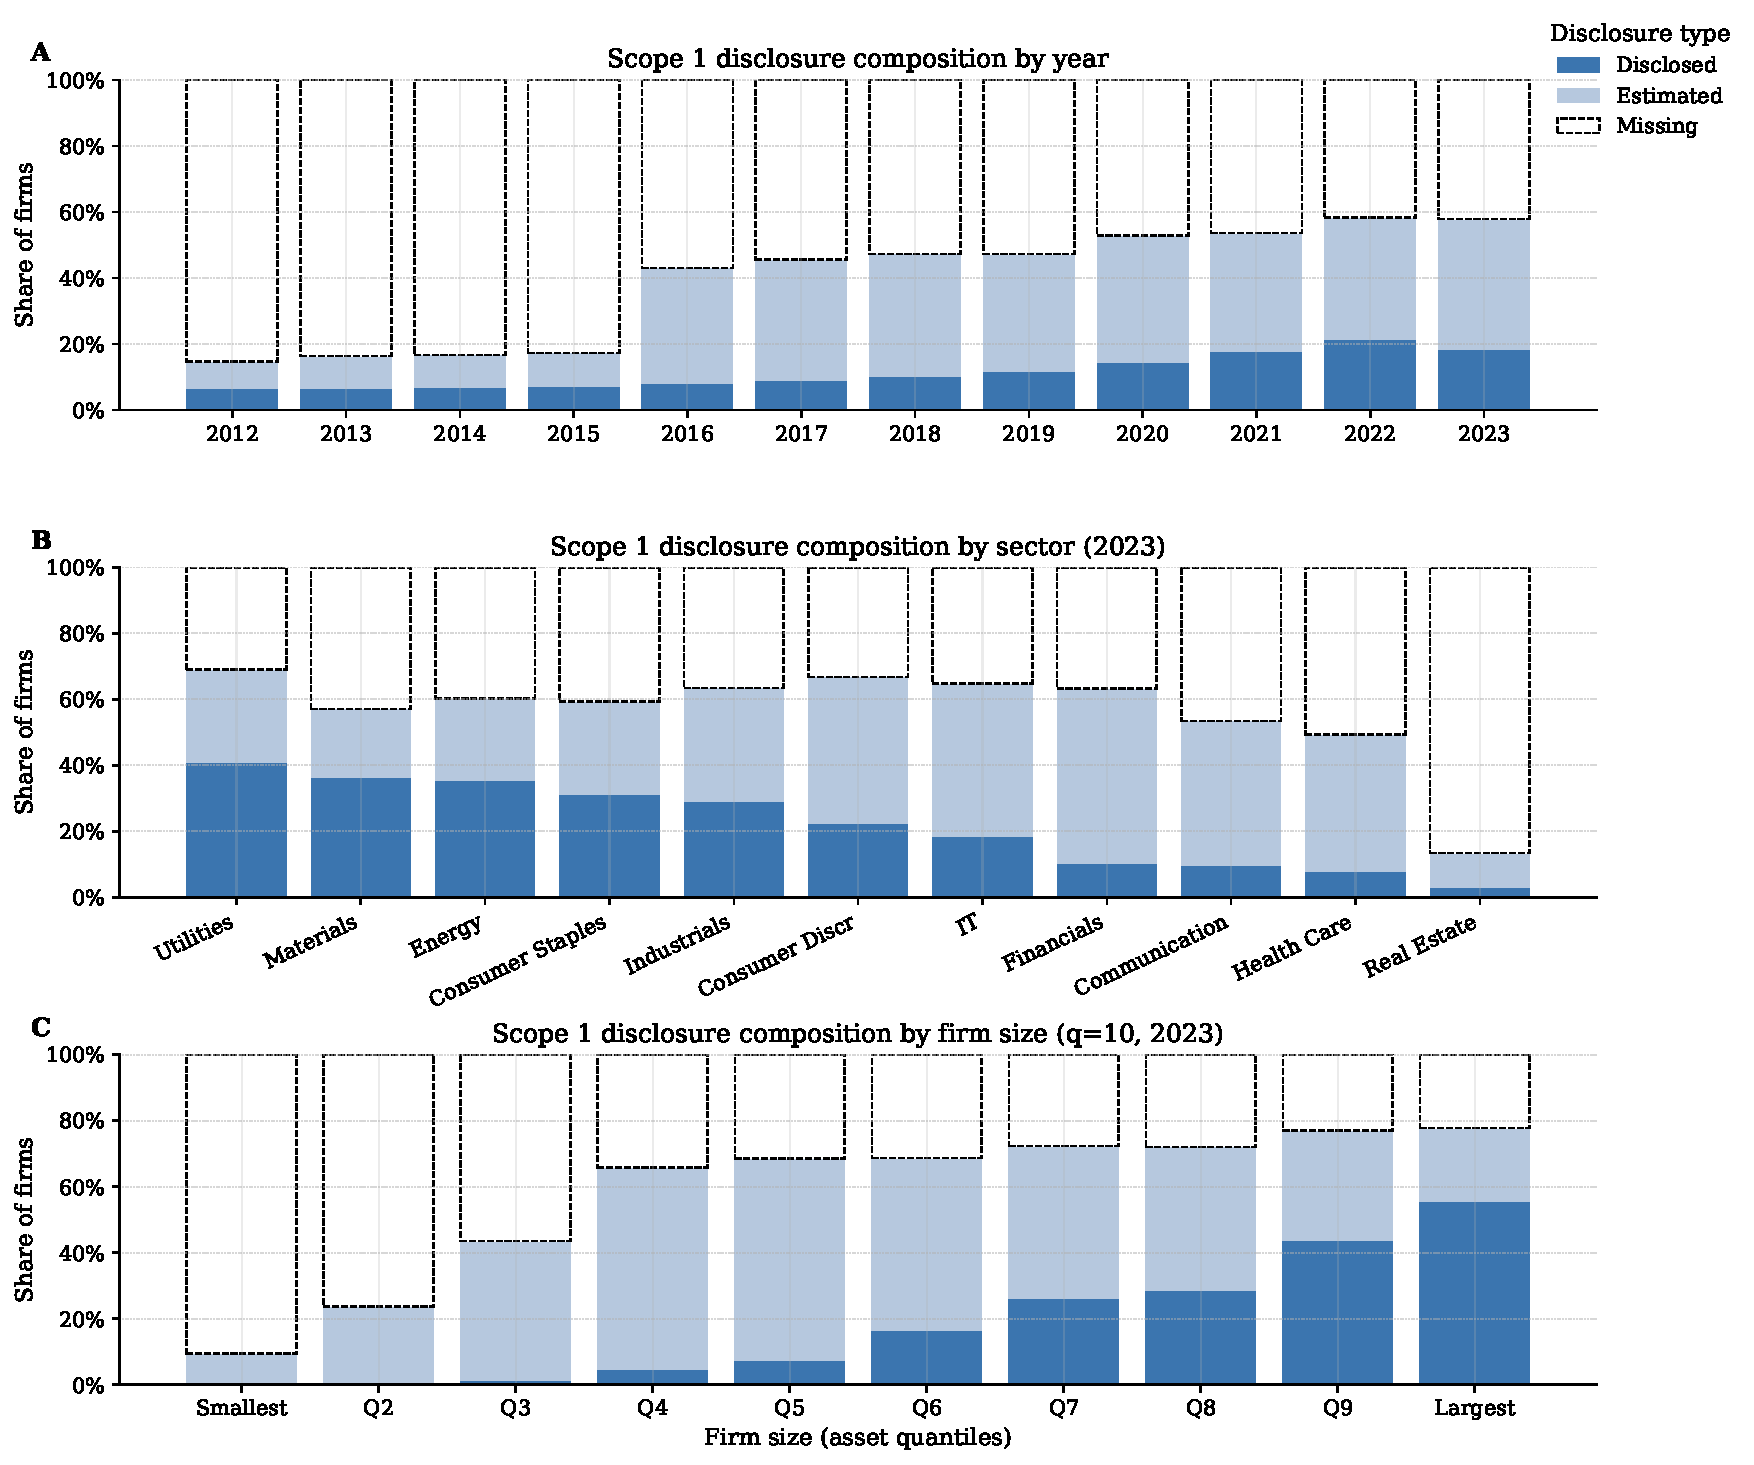
\includegraphics[width=0.9\linewidth]{figs/fig1_disclosure.pdf}
    \caption{\textbf{Scope~1 emissions disclosure composition.} Each bar partitions firms into three mutually exclusive groups -- \emph{disclosed} (firm-reported emissions; dark blue), \emph{estimated} (Trucost vendor estimate; light blue), and \emph{missing} (Compustat firms with no Trucost coverage; dashed outline) -- as a share of firms summing to 100\% within each bar. \textbf{Panel A} plots the composition by year over 2012--2023; \textbf{Panel B} the 2023 composition by GICS sector; and \textbf{Panel C} the 2023 composition by firm-size decile (asset quantiles, smallest to largest). Data are from S\&P Trucost Environmental merged onto the Compustat universe of U.S.\ public firms.}
    \label{fig:disclosure_trends}
\end{figure}

The bottom panel reports disclosure rates by firm-size decile, measured by total assets. Larger firms are substantially more likely to disclose emissions or to be covered by Trucost estimates, whereas coverage among smaller firms remains limited. In the bottom two deciles, fewer than 25\% of firms have any emissions data available, and direct disclosure is essentially absent. In contrast, firms in the top deciles exhibit total coverage exceeding 50\%, with direct reporting accounting for a large and rising share.

Together, these patterns highlight systematic variation in emissions disclosure across time, sectors, and firm size, underscoring the importance of accounting for selective disclosure in empirical analyses. In the next section, we describe the empirical framework used to address this selection when imputing missing emissions.


% ============================================================
\section{Recovering Latent Emissions}
\label{sec:methodology}
\label{sec:measurement}

We recover Scope~1 emissions for every firm in the Compustat universe by correcting the disclosed-firm distribution for non-ignorable selection. Guided by the model of Section~\ref{sec:theory}, the procedure has five steps: (i) an outcome model fit on disclosers; (ii) a baseline missing-at-random (MAR) imputation of non-disclosers from that model; (iii) a logistic disclosure model whose emissions slope is the selection severity index $\gamma$; (iv) the exponential-tilt correction of Corollary~\ref{cor:expo_tilt}, applied to the baseline draws; and (v) Monte Carlo propagation of imputation uncertainty. This section sketches each step and reports what it delivers; the granular choices -- functional forms, the imputation draw, the formal exclusion restriction, and the Monte Carlo algorithm -- are collected in Appendix~\ref{app:methods}. 

\begin{figure}[htbp]
    \centering
    \resizebox{\textwidth}{!}{%
    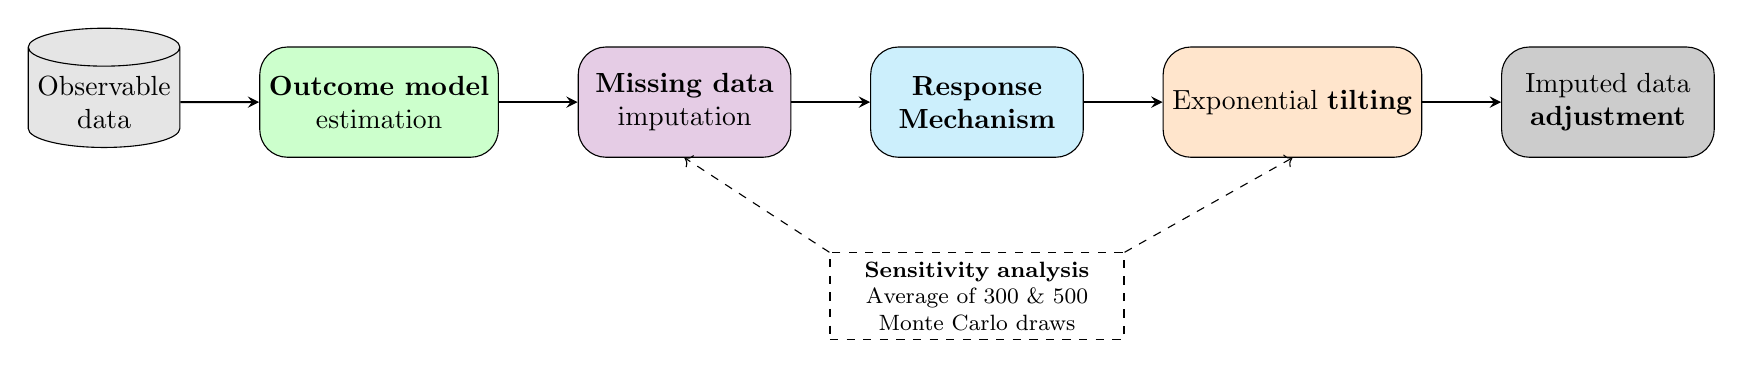
\begin{tikzpicture}[node distance=1cm and 1cm]

    \tikzstyle{data} = [cylinder, shape border rotate=90, aspect=0.25, draw, fill=gray!20, text centered, minimum height=3em]
    \tikzstyle{process} = [rectangle, rounded corners=10pt, minimum width=2.7cm, minimum height=1.4cm, text centered, draw, fill=none]
    \tikzstyle{arrow} = [thick, ->, >=stealth]
    \tikzstyle{note} = [rectangle, draw=black, dashed, fill=white, text width=3.5cm, align=center, font=\footnotesize]

    \node (data) [data, align=center] {Observable \\ data};
    \node (step1) [process, right=of data, fill=green!20, align=center] {\textbf{Outcome model}  \\ estimation};
    \node (step2) [process, right=of step1, fill=violet!20, align=center] {\textbf{Missing data} \\ imputation};
    \node (step3) [process, right=of step2, fill=cyan!20, align=center] {\textbf{Response} \\ \textbf{Mechanism}};
    \node (step4) [process, right=of step3, fill=orange!20] {Exponential \textbf{tilting}};
    \node (step5) [process, right=of step4, fill=gray!40, align=center] {Imputed data \\ \textbf{adjustment}};

    \draw [arrow] (data) -- (step1);
    \draw [arrow] (step1) -- (step2);
    \draw [arrow] (step2) -- (step3);
    \draw [arrow] (step3) -- (step4);
    \draw [arrow] (step4) -- (step5);

    \node (note) [note, below=1.2cm of step3] {\textbf{Sensitivity analysis} \\ Average of 300 \& 500 \\ Monte Carlo draws};
    \draw[dashed,->] (note.north west) -- (step2.south);
    \draw[dashed,->] (note.north east) -- (step4.south);

    \end{tikzpicture}
    }
    \caption{Workflow of the missing data imputation methodology. The procedure consists of five main steps: (1) outcome modeling based on observable data; (2) imputation of missing values; (3) estimation of the response mechanism; (4) application of exponential tilting; and (5) adjustment of the imputed values. Additionally, a sensitivity analysis is conducted using Monte Carlo simulations with 300 and 500 random draws, respectively.}
    \label{fig:missing-data-workflow}
\end{figure}

\subsection{Outcome model}
\label{subsec:outcome}

The first step estimates the conditional distribution of emissions among disclosers with a lognormal model,

\begin{equation}
\label{eq:outcome_model}
y_{it} = \eta_0 + \eta_1 \log \mathrm{assets}_{it} + \eta_2\, z_{it} + \mu_{j(i)} + \tau_t + \varepsilon_{it}, \qquad \varepsilon_{it} \sim \mathcal{N}(0, \sigma^2),
\end{equation}
where $y_{it}$ is log Scope~1 emissions of firm $i$ in year $t$, $\mathrm{assets}_{it}$ is total assets (a proxy for production scale, without the valuation-driven volatility of market capitalization), $z_{it}$ is the oil-price exposure shifter used for identification (Section~\ref{subsec:disc_mech}), and $\mu_{j(i)}$ and $\tau_t$ are GICS industry and year fixed effects, respectively. We use total assets to proxy production scale without valuation-driven volatility. Fit on disclosers, the model recovers the production-side signal in emissions -- scale, industry technology, aggregate conditions -- and supplies the conditional density $f_1(y\mid\mathbf{x})$ from which we draw baseline MAR imputations for non-disclosers (the draw is given in Appendix~\ref{app:methods}). These draws treat non-disclosers as if $f_0(y\mid\mathbf{x}) = f_1(y\mid\mathbf{x})$ -- the MAR benchmark that Proposition~\ref{prop:mnar_bias} shows fails whenever $\gamma \neq 0$; the remaining steps correct it.

Table~\ref{tab:OutcomeModel_baseline_wti_gind} presents the estimated coefficients from our model. All covariates, with the exception of a few year indicators, are statistically significant at the 5\% level. The model explains a substantial portion of the variance in reported CO$_2$ emissions, with an adjusted $R^2$ of 0.81. 

Firm size, proxied by log assets, shows a strong positive association with Scope 1 emissions. The coefficient estimate of 0.97 suggests that a 1\% increase in firm size is associated with approximately a 0.97\% increase in emissions, scaling almost linearly. The exposure shifter enters positively and strongly ($\hat\eta_2 = 0.19$, $t\approx 32$): among physically exposed firms, emissions co-move with the oil price, as expected when fuel-combustion operations scale with energy costs. The coefficient is a relevance statistic rather than a structural parameter — it is the first-stage requirement that the instrument shift emissions — and its strength ($t>30$) rules out weak-instrument concerns.
    
Industry differences in emissions are substantial. Differentials are estimated relative to the omitted industry, and the great majority are significant at the 1\% level. The largest positive differentials fall on the most physically fuel-intensive industries: Passenger Airlines and Marine Transportation (about $+2.3$), Electric and Multi-Utilities ($+1.5$ to $+1.8$), Chemicals and other Materials ($+1.0$ to $+1.7$), and Oil, Gas \& Consumable Fuels. The most negative are the asset-light service industries: Capital Markets, Consumer Finance, and Insurance cluster near $-5$, and Software, IT Services, Interactive Media, and Professional Services lie between $-3.5$ and $-4.2$. The finer resolution also reveals contrasts invisible at the sector level: within Utilities, Electric Utilities load strongly positive ($+1.8$) while Water Utilities are sharply negative ($-3.0$). Overall, this pattern is consistent with the broad distinction between more emission-intensive (\textit{brown}) and less emission-intensive (\textit{green}) sectors, reflecting structural differences in business operations and energy use.

The year fixed effects from the indicate a clear and statistically significant downward trend in reported Scope 1 emissions conditional on firm characteristics over the past decade. Using 2012 as the reference year, the coefficients for subsequent years become increasingly negative, with effects growing in magnitude and statistical significance over time. While early-year coefficients (2013–2016) are small and not statistically different from zero, the decline becomes significant starting in 2018. By 2023, the coefficient reaches -0.69, implying that, all else equal, reported emissions in 2023 were approximately 50\% lower than the 2012 baseline. This sustained decline likely reflects a combination of structural changes, including tightening climate regulation, increased stakeholder scrutiny, and improvements in emissions measurement and reporting. The accelerating pace of change after 2018 may also coincide with major global climate initiatives and improved emissions tracking mechanisms. These time effects offer strong evidence that the landscape of corporate emissions disclosure has evolved materially over the time frame considered.

Following our methodology, the estimated outcome model is used to generate plausible values for missing emissions data by randomly drawing from the predictive distribution in Equation (\ref{eq:outcome_model}). This forms the first step of the imputation process, to obtain a complete dataset that will be utilized to model the response mechanism. 

\subsection{Disclosure mechanism and the selection severity index}
\label{subsec:disc_mech}

After imputing scope 1 emissions, we proceed to estimate the response propensity for each company, leveraging the complete covariates $\textbf{x}_1$ and the dependent variable $y$. We model the disclosure decision with a logistic response mechanism in firm characteristics and emissions,

\begin{equation}
\label{eq:response_model}
\mathbb{P}(\delta_i = 1 \mid \mathbf{x}_{1i}, y_i)
= \frac{\exp\{ f(\mathbf{x}_{1i}) + g(y_i) \}}{1 + \exp\{ f(\mathbf{x}_{1i}) + g(y_i) \}},
\end{equation}

the empirical counterpart of the equilibrium propensity of Theorem~\ref{thm:existence}. Our primary specification is fully parametric, with $f$ and $g$ linear, so $g(y_i) = -\gamma y_i$ and the coefficient on $y_i$ estimates $-\hat\gamma$ directly. This is the specification the model implies: the disclosure cost is linear in emissions, so the equilibrium propensity is linear in $y$ (Lemma~\ref{lemma:indiv_best_resp}). A semiparametric variant with penalized splines relaxes that linearity as a robustness check \citep{yang2017semiparametric}; its specification and results are in Appendix~\ref{app:methods}.

Identification of the emissions slope is the crux: $y_i$ is unobserved for exactly the non-disclosers the model describes, so it cannot come from the disclosing sample alone. Identification rests on an \emph{excluded shifter} of emissions \citep{wang2014instrumental}, and we build one in shift-share (Bartik) form -- an aggregate shock interacted with predetermined firm-level exposure \citep{goldsmithpinkham2020bartik, borusyak2022quasi}:
\begin{equation}
\label{eq:instrument}
z_{it} = \log(\mathrm{WTI}_t) \times \mathrm{exposure}_i ,
\end{equation}
where $\mathrm{WTI}_t$ is the crude oil price and $\mathrm{exposure}_i$ is firm $i$'s predetermined physical-capital intensity: gross property, plant, and equipment over total assets, averaged over the firm's first (up to) five non-missing sample years and then held fixed. Averaging the first few years rather than taking a single year reduces the influence of one anomalous observation on a firm-level weight that is applied throughout the panel; because the exposure is time-invariant by construction, all within-firm time variation in $z_{it}$ comes from the oil price. Because $z_{it}$ varies across firms \emph{within} a year, it is not collinear with the year fixed effects, and so -- unlike the aggregate oil price alone, which the year effects absorb -- it supplies identifying variation present in the emissions equation but excluded from the disclosure equation. It is \emph{relevant}: oil-price movements shift the emissions of physically exposed firms more, and $z_{it}$ enters the outcome model~\eqref{eq:outcome_model} strongly (coefficient $0.19$, $t \approx 32$). Physical-capital intensity is the economically appropriate exposure because Scope~1 emissions are, by construction, direct emissions from combustion in owned equipment: a firm's installed property, plant, and equipment scales the fuel it burns on site, and it is through that plant that the oil price reaches its emissions. More immediate proxies -- energy intensity, fuel purchases -- would be contaminated for identification precisely because they are themselves choices that respond to the oil price and to the firm's contemporaneous decisions; predetermined PP\&E, fixed at its pre-sample value, is an exposure that is both economically apt and not itself a function of the shock.

Exclusion is the identifying assumption, and it is worth stating exactly, because it is weaker than the econometrics might suggest. We do not require that oil prices be exogenous to firm value; they plainly are not. We require only that, conditional on year fixed effects and the size and sector controls, the interaction of the aggregate oil price with predetermined physical-capital intensity affect the disclosure \emph{decision} only through its effect on \emph{emissions}. The design accounts for the natural alternative channels rather than assuming them away. Any effect of the oil price common across firms -- shifting expected regulation, financing conditions, or investor attention to carbon -- is absorbed by the year fixed effects; any effect operating at the sector level is absorbed by the sector controls. What is left to identify $\gamma$ is the difference, \emph{within} a year and sector, between the disclosure choices of firms that are more and less physically exposed to the oil price. For that residual variation to violate exclusion, physical intensity would have to move disclosure through a firm-level channel that is neither common, nor sector-wide, nor the emissions the shifter shifts -- most plausibly through profitability, if oil-price gains raised the cash flows of exposed firms and cash flow independently drove disclosure. Because profitability and size are closely tied, conditioning the propensity on size already absorbs much of this channel. More tellingly, a sensitivity analysis that allows the shifter a direct effect on disclosure \citep{conley2012plausibly} shows that the plausible violation works \emph{against} the result rather than for it: a direct effect of the sign that profitability or investor attention would induce only \emph{raises} $\hat\gamma$, and overturning $\gamma>0$ would require a wrong-signed channel several times the shifter's own association with disclosure (Appendix~\ref{app:methods}). Appendix~\ref{app:methods} also states the restriction formally and reports an over-identification check -- three shifters built from different shocks, vendors, and markets recover the same $\gamma$, which they would not if each violated exclusion through its own channel -- and Appendix~\ref{app:robustness} reports the estimates when the oil shock is replaced by U.S.\ real GDP.

The estimate is signed as the model predicts (Table~\ref{tab:results_LM}): $\hat\gamma = 0.199$ ($B=500$; $0.195$ at $B=300$), positive and significant at the 1\% level -- higher emitters are systematically less likely to disclose. This is direct empirical support for non-ignorable disclosure and a measured value of the structural selection severity of Theorem~\ref{thm:existence}. Coefficients are standardized, so magnitudes read as the effect of a one-standard-deviation move evaluated at the sample disclosure rate of 13.0\%. A one-standard-deviation increase in firm size raises the disclosure probability from 13.0\% to approximately 49\%: larger firms are far more likely to report, which is the dominant force in the disclosure decision and the reason $f(\mathbf{x})$ must absorb size before the emissions slope is interpretable. Conversely, a one-standard-deviation increase in Scope~1 emissions lowers the disclosure probability from 13.0\% to approximately 10.9\%, a relative decline of about 16\%, consistent with higher-emitting firms withholding their environmental performance.

The emissions coefficient carries larger sampling uncertainty than the other covariates (standard error $0.074$, versus $0.028$ on size), which is expected: $y_i$ is imputed for the non-disclosers whose behavior identifies $\gamma$, and the Monte Carlo propagates that imputation uncertainty into the slope. Carrying the 95\% interval through the logistic transformation, the implied disclosure probability at $+1$ SD of emissions ranges from about 9.6\% to 12.4\% -- everywhere below the 13.0\% base rate, so the \emph{sign} of the selection effect is stable across the interval even though its magnitude is not sharply pinned down. This is the appropriate degree of confidence to attach to the pooled estimate: the direction of strategic silence is firm, its exact strength less so, and Section~\ref{subsec:boundary} shows that the pooled number in any case averages over sectors and ownership structures whose selection severities differ by an order of magnitude and in sign.


\subsection{The tilting correction and its distributional effect}
\label{subsec:tilting_adj}

With $\hat\gamma$ estimated, we correct the baseline imputations by the exponential tilt of Corollary~\ref{cor:expo_tilt}, reweighting each draw by
\begin{equation}
\label{eq:tilting_weights}
w_i \propto \exp\{\hat\gamma\, \hat{y}_i\},
\end{equation}
so that firms with lower disclosure probabilities -- the higher emitters -- receive more weight, restoring the upper-tail mass that selection removes. The idea is that forecasted emissions from the outcome model are scaled based on the inverse likelihood of disclosure: the less likely a firm is to report, the greater the upward adjustment. However, the final tilt does not depend only on disclosure probability but also on each company's size, business sector, and imputed emissions. Hence, a low reporting probability does not always result in a large adjustment. 

% We propagate imputation uncertainty by Monte Carlo, redrawing, re-estimating, and re-tilting over $B\in\{300,500\}$ draws \citep{gohil2020multiple}; because the MNAR restriction is untestable and the tilt compounds any misspecification \citep{little2019statistical}, this quantifies sampling and specification variability rather than testing the assumption (Appendix~\ref{app:methods}).

The correction is economically large (Table~\ref{tab:emissions_tilts}). Relative to the MAR baseline mean of 957{,}284 tCO$_2$, the fully parametric tilt raises average imputed Scope~1 emissions to 1{,}075{,}583 tCO$_2$, an uplift of 12.4\% ($B=500$; 11.9\% at $B=300$). The semiparametric response model, which relaxes the linearity of $g(y)$, produces a larger correction of 19.1\% (1{,}139{,}831 tCO$_2$); we report the fully parametric figure as the headline because it is the specification the model implies, and read the semiparametric number as an upper bound that indicates the correction is not an artifact of the linear functional form. Under both, the correction concentrates in the upper tail rather than shifting the distribution uniformly, as the transition-firm validation below confirms; and because the tilt reweights toward high emitters, the recovered aggregate depends more on which upper-tail firms a given imputation draws, so the across-draw standard deviation of the mean roughly doubles (46{,}054 to 86{,}510 under FP). Because the overwhelming majority of firms are silent, this compounds into an upward revision of aggregate emissions (Section~\ref{subsec:aggregate}): conventional MAR imputation understates corporate emissions precisely where the level matters most for aggregate damages.

\subsection{Validation: firms transitioning to disclosure}
\label{subsec:validation}

A fundamental challenge in non-ignorable missingness settings is the absence of ground truth for validating imputed values. However, a subset of firms in our sample transition from non-disclosure to disclosure over time, providing an opportunity for external validation. Specifically, we identify 633 companies for which emissions were initially estimated, and then disclosed in subsequent years. For these firms, we compare emissions imputed in the year \textit{prior} to disclosure with the subsequently reported values. This is a calibration diagnostic, not identification: the transition firms play no role in estimation. 

\begin{figure}[htbp]
\centering
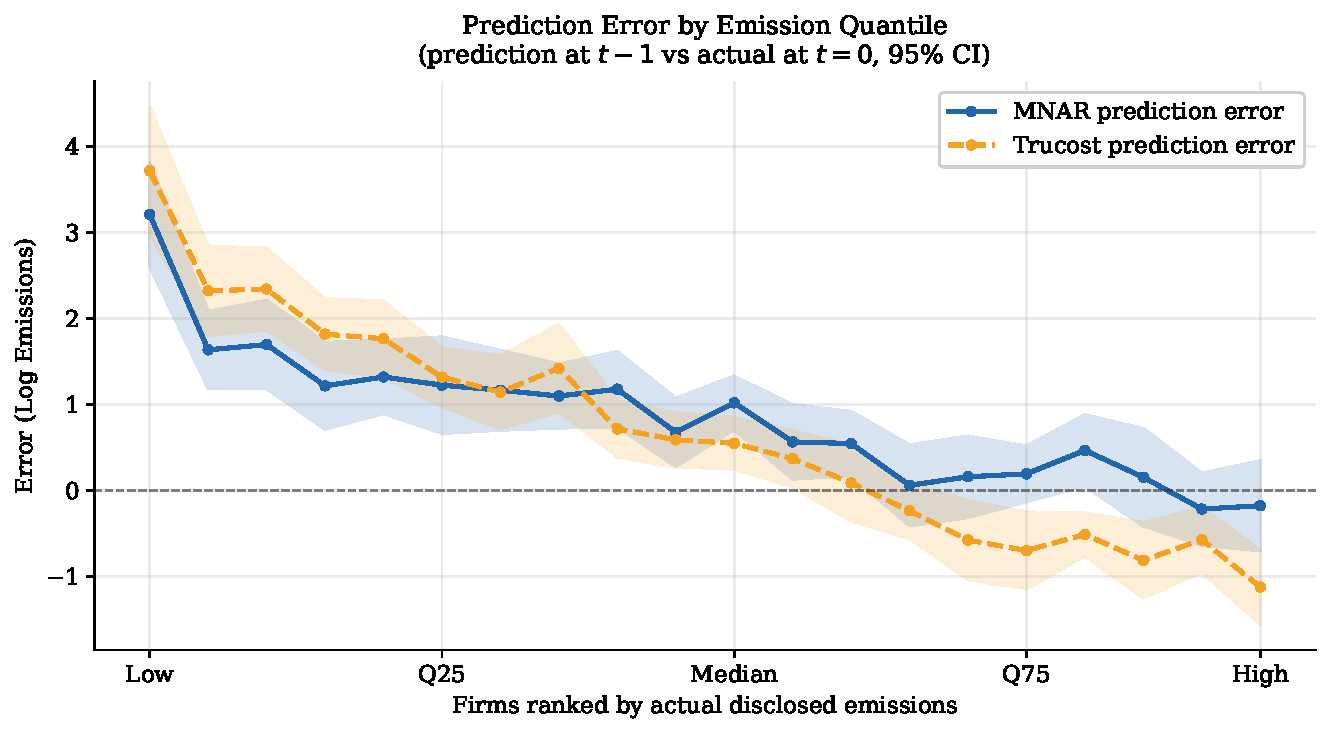
\includegraphics[width=0.75\linewidth]{figs/validation_error_quantile.pdf}
\caption{\textbf{Transition-firm validation: prediction error by emissions quartile.} For the 633 firms that transition into disclosure, the plot shows the prediction error (log predicted minus log subsequently-disclosed Scope~1 emissions), measured in the year before disclosure, by quartile of disclosed emissions. MNAR-corrected imputations versus Trucost vendor estimates; positive values indicate overstatement. The MNAR correction is nearly unbiased in the top quartile, where Trucost understates emissions by about 0.7 log units.}
\label{fig:validation_error_quantile}
\end{figure}


The MNAR-corrected imputations track the disclosed ranking more closely than the vendor estimates (Spearman $\rho = 0.86$ versus $0.81$ for Trucost), and the gain concentrates exactly where it matters. Among the highest-emitting quartile, the MNAR prediction is essentially unbiased (mean log error $+0.07$), whereas Trucost understates emissions by about $0.74$ log units -- roughly 50\% -- precisely the upper-tail firms that dominate aggregate emissions. Both methods overstate the smallest emitters, an unavoidable feature of conditional-mean imputation for near-zero values, but those firms are negligible for aggregates; the accuracy that matters for aggregate emissions and damages is in the tail, where the correction excels (Figure~\ref{fig:validation_error_quantile}). This pattern is consistent with our framework's design, which accounts for strategic non-disclosure incentives that are more prevalent among large emitters. Given that these firms contribute disproportionately to aggregate pollution, the reduction in high-end underestimation is critical for accurately estimating the total average emissions and associated carbon damages. 

Together, these steps deliver a Scope~1 emissions figure for every firm in the Compustat universe, including the majority that never disclose. Relative to Trucost estimates the recovered distribution is materially heavier in the upper tail, and the transition-firm validation confirms that the correction bites where it should -- among the high emitters that dominate aggregates.

\subsection{Aggregate emissions and carbon damages}
\label{subsec:aggregate}

Because the recovered measure exists for every firm, it can be summed. This is where the correction has its largest consequence and, we should say at the outset, where it should be read most cautiously: an aggregate is a sum over the upper tail, and the upper tail is exactly where the imputation is most extrapolated. We report aggregate quantities as illustrative magnitudes rather than as precise estimates, and we guard the sum against its most fragile component by capping each imputed value at the largest emissions figure any firm actually discloses in that year, on the reasoning that no non-discloser should be assigned more carbon than the largest firm that reports.\footnote{The cap binds on a handful of firm-years -- in 2022, two non-disclosers carry uncapped imputed values above the largest disclosed emitter, one of them at more than twice it -- but because a sum is dominated by its extreme terms, those few firms matter: the uncapped 2022 total is $9.5\%$ above the missing-at-random baseline and the capped total $4.4\%$. We report the capped figures throughout.}

On the capped series, aggregate Scope~1 emissions for the major-exchange universe are approximately $3.5$ GtCO$_2$ in 2022, $4.4\%$ above the missing-at-random baseline that ignores selection. The revision is modest in proportional terms because the disclosed and vendor-covered firms that dominate the aggregate are largely unaffected by the correction; it is concentrated among the non-disclosers, whose recovered emissions the missing-at-random benchmark understates.

The economically larger point is a comparison of levels. Following \citet{greenstone2023mandatory}, we value emissions at the social cost of carbon under their low, mid, and high scenarios (\$51, \$190, and \$250 per tCO$_2$) and express corporate carbon damages as a share of firm revenue, which normalizes for size and, usefully, renders the aggregate insensitive to the tail cap -- the capping that moves the emissions total by several percentage points moves the damages ratio by less than one, because the largest emitters carry correspondingly large revenues. For 2019, the year for which \citet{greenstone2023mandatory} report damages for the S\&P~1500, our estimates are more than double theirs at every scenario (Table~\ref{tab:carbon_damages}): at the mid social cost, damages are $4.6\%$ of revenue under the fully parametric correction and $4.9\%$ under the semiparametric, against their $2.0\%$.

\begin{table}[htbp]
\footnotesize\centering
\caption{\textbf{Corporate carbon damages as a share of revenue, 2019.} Damages
are Scope~1 emissions valued at the social cost of carbon under the three
scenarios of \citet{greenstone2023mandatory} (\$51, \$190, \$250 per tCO$_2$),
aggregated and divided by aggregate revenue. The first row reproduces their
S\&P~1500 benchmark; the lower rows use our recovered emissions for the
major-exchange universe under the fully parametric and semiparametric
corrections. Imputed values are capped at the largest disclosed emitter, though
the ratio is nearly unchanged without the cap.}
\label{tab:carbon_damages}
\begin{tabular}{lccc}
\toprule
 & Low (\$51) & Mid (\$190) & High (\$250) \\
\midrule
\citet{greenstone2023mandatory}, S\&P 1500 & 0.5\% & 2.0\% & 2.7\% \\
\midrule
Recovered universe, fully parametric & 2.5\% & 4.6\% & 6.1\% \\
Recovered universe, semiparametric   & 2.6\% & 4.9\% & 6.4\% \\
\bottomrule
\end{tabular}
\begin{flushleft}\footnotesize
\textit{Notes:} Multiples relative to the benchmark are $2.2$--$2.6\times$ across
scenarios and corrections. The gap is a sample-breadth effect: the major-exchange
universe reaches well beyond the S\&P~1500 into smaller and more carbon-intensive
firms, which disclose least and which the recovered measure is designed to
capture.
\end{flushleft}
\end{table}

We read this multiple as a statement about coverage, not about the social cost of carbon itself, which is common to both rows. Our sample extends beyond the large, visible firms of the S\&P~1500 to the smaller and more carbon-intensive firms that make up most of the non-disclosing majority, and it is their damages -- absent from any disclosed-sample accounting -- that roughly double the total. The understatement in conventional figures is thus not uniform: it is concentrated in precisely the firms with the strongest incentive to stay silent, which is the same conclusion the selection model reaches from the disclosure side.

With emissions in hand for disclosers and non-disclosers alike, we can finally separate two objects the prior literature was forced to conflate: the pricing of the emissions \emph{level} and the pricing of the disclosure \emph{decision}. Section~\ref{sec:pricing} turns to that separation -- and to the boundary conditions under which strategic silence is priced at all.


% ============================================================
\section{Selection Severity and its Boundary Conditions}
\label{sec:mechanism}

Section~\ref{sec:measurement} estimated the selection severity index and used it to recover emissions for the firms that stay silent. This section asks where that severity is large, and when. Both questions are about the disclosure decision rather than about prices: they are answered from the same propensity model, on the same annual panel, and the evidence is behavioural throughout. Section~\ref{subsec:boundary} locates strategic silence in the cross-section, showing that it operates only where an audience exists and only where there is something to hide; Section~\ref{subsec:regime} follows the severity over time.

\subsection{Boundary conditions: where strategic silence operates}
\label{subsec:boundary}

Voluntary disclosure theory predicts that strategic silence is informative only when an audience interprets it as bad news \citep{milgrom1981good, verrecchia1983discretionary}. Proposition~\ref{prop:gamma} makes this a sign condition: $\gamma_{\text{eff}} > 0$ where scrutiny dominates, $\gamma_{\text{eff}} < 0$ where a transparency benefit dominates instead. We test it by re-estimating the emissions slope separately within observable settings that proxy for the presence of an audience, holding sector and year fixed effects throughout.\footnote{Throughout this subsection $\hat\gamma$ is reported in the sign convention of the model, so that $\hat\gamma > 0$ denotes strategic silence (higher emitters disclose less) and $\hat\gamma < 0$ denotes reverse selection. Emissions are standardized within sector, so magnitudes are log-odds per within-sector standard deviation and are comparable across groups whose emission scales differ by orders of magnitude.} Our proxy for the audience is institutional ownership: concentrated institutional holders monitor the firms they hold, face climate-reporting obligations of their own, and can price what they infer from silence. Two features of the design follow, and we state them before the results.

First, we sort firms into ownership terciles \emph{within} sector rather than comparing sectors to one another. This is not a stylistic preference but a requirement of the question. Sectors are nearly homogeneous in institutional ownership: mean ownership runs from only $0.56$ to $0.70$ across the eleven GICS sectors, so essentially all of the variation in who is watching a firm is variation \emph{within} an industry rather than between industries. A between-sector comparison could not isolate the audience even in principle, because across sectors the audience scarcely differs while everything else -- production technology, measurement infrastructure, reporting norms, mandated coverage -- differs a great deal. Appendix~\ref{app:robustness} reports the sectoral cut for completeness and explains why we read it as descriptive.

Second, size enters with a tercile-specific slope. Firm size is the dominant determinant of disclosure and is strongly correlated with emissions, so a size coefficient constrained to be common across groups is absorbed by the very emissions slope the exercise is meant to read. Here the restriction turns out to be benign -- estimated freely, the size slope spans only a factor of $1.25$ across terciles, precisely because terciles are formed within sector and production technology is roughly held fixed -- and the results are nearly identical either way. We free it regardless. In the sectoral cut, where the same restriction spans a factor of $64$, imposing it reverses the sign of $\hat\gamma$ in two sectors; that contrast is itself a reason to prefer the within-sector design.

\paragraph{Ownership channel.} We measure institutional ownership from quarterly
13F filings. For each firm-quarter we aggregate the shares held by all reporting
institutions and scale by shares outstanding, 

\begin{equation}
    \mathrm{io}_{iq} = \sum_m
\mathrm{shares}_{imq} / \mathrm{shrout}_{iq},
\end{equation} 

taking the denominator from CRSP at the same month-end as the 13F report date so that numerator and denominator refer to the same point in time.\footnote{Holdings are from Thomson Reuters 13F via WRDS. Because 13F reports by CUSIP while Compustat identifies firms by GVKEY, we link
GVKEY to PERMNO through the CRSP/Compustat Merged link table and PERMNO to its historical eight-digit CUSIP through CRSP \texttt{stocknames}, matching on
date ranges at both steps: CUSIPs change over a firm's life, and an unbounded merge would attribute holdings to the wrong entity after a restructuring or
spin-off. We cap $\mathrm{io}_{iq}$ at $1.5$; ratios above one arise mechanically from short positions and stale filings rather than from genuine over-ownership.} The annual measure $\mathrm{io}_{it}$ averages the quarter-end ratios within the
year; 90\% of firm-years have all four quarters. Ownership is available for 42{,}310 of the 51{,}355 firm-years in the estimation sample (82\%), with coverage between 74\% and 90\% in every year and no trend that would tilt the full-window comparison.

We sort firms into terciles of $\mathrm{io}_{it}$ \emph{within sector}, so that the proxy captures how closely held a firm is relative to its own industry peers rather than reproducing cross-sector differences in ownership norms. The resulting groups
are well separated: mean ownership is $0.21$ in the bottom tercile, $0.68$ in the middle, and $0.95$ in the top. Estimating one emissions slope per tercile,
Figure~\ref{fig:gamma_by_io} shows the pattern the model predicts.

\begin{figure}[htbp]
    \centering
    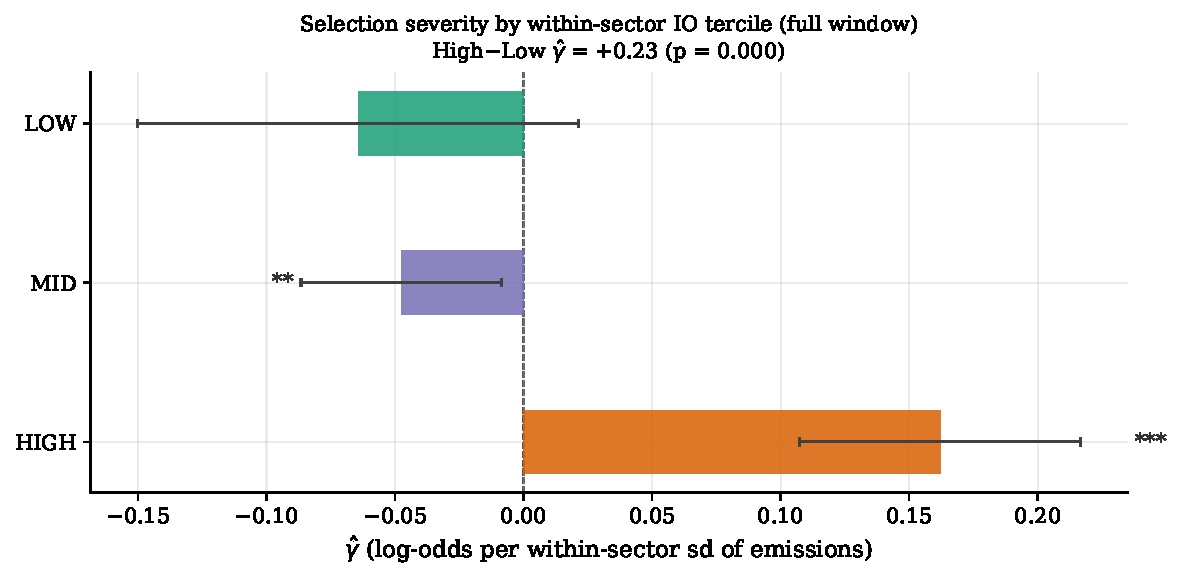
\includegraphics[width=0.95\linewidth]{figs/gamma_by_io_fullwindow_tilt_test.pdf}
    \caption{\textbf{Selection severity by institutional ownership.} Estimated $\hat\gamma$ from a disclosure propensity model in which the emissions slope is interacted with within-sector institutional-ownership terciles, with 95\% confidence intervals. Emissions are standardized within sector, so $\hat\gamma$ is in log-odds per within-sector standard deviation. Positive $\hat\gamma$ indicates strategic silence: higher emitters are less likely to disclose. The specification includes sector, year, and ownership-tercile fixed effects, and allows the size slope to differ by tercile. Stars denote significance at the 10\%, 5\%, and 1\% levels.}
    \label{fig:gamma_by_io}
\end{figure}

Selection is present, and strongly so, only where ownership is concentrated: $\hat\gamma = +0.162^{***}$ in the top tercile, against $-0.048^{**}$ in the middle and $-0.064$ (insignificant) at the bottom. The robust fact is the difference, $+0.226$ (s.e.\ $0.052$, $p<0.001$): moving from the bottom to the top of the within-sector ownership distribution changes the sign of the emissions--disclosure relation. The bottom tercile on its own is imprecise: its point estimate is negative, consistent with reverse selection, but it carries $p = 0.14$, and the significant negative estimate sits in the middle tercile. So the data establish that selection does not merely \emph{weaken} as monitoring falls away -- the estimates go negative rather than to zero -- while a strict reversal at the very bottom is suggestive rather than decisive.

Even so, the test discriminates. This is Proposition~\ref{prop:gamma} operating near the boundary $b = \beta + c_1$: where no audience penalizes revealed emissions, the transparency benefit $b$ dominates and $\gamma_{\text{eff}}$ falls, in these estimates to zero or below. A rival account in which disclosure costs simply scale with firm sophistication predicts that selection attenuates smoothly as ownership falls; it does not predict that the relation crosses zero in the two lower terciles while turning sharply positive in the top one.


\paragraph{Isolating the institutional ownership channel.} Institutional holders concentrate in firms that are larger, more liquid, more likely to be index constituents, and potentially better equipped to measure and report their own emissions. Any of these characteristics could generate an ownership gradient in $\hat\gamma$ even if institutional investors played no role in the disclosure decision. The question is therefore whether the ownership gradient reflects an \emph{audience} that interprets non-disclosure, or simply greater \emph{disclosure capacity} among firms with concentrated institutional ownership. The two mechanisms make different predictions. The audience mechanism operates only when silence conceals unfavorable information: if a firm has little carbon to hide, non-disclosure carries no adverse signal. It therefore predicts an ownership gradient only among high-emitting firms. By contrast, the disclosure-capacity mechanism imposes no such condition. If concentrated ownership merely proxies for the sophistication to measure and report emissions, the ownership gradient should appear regardless of a firm's emissions. The empirical prediction is therefore not about the average level of $\hat\gamma$, but about its interaction with firms' ex ante carbon intensity. A triple-difference design separates the two mechanisms.

We split the sample a second time, on how much a firm plausibly has to hide, and estimate one emissions slope in each of the four ownership-by-brownness cells. Brownness has to be measured from observed data alone: conditioning on the recovered emissions vector would condition on the output of the same model that produces $\hat\gamma$, and any pattern so obtained would be partly mechanical. We use instead the carbon intensity of a firm's GICS industry as revealed by the firms in it that \emph{do} disclose -- the median of reported Scope~1 emissions over revenue among disclosers -- assigned to every firm in that industry, and split at the median. A firm's own disclosure choice cannot move its industry's median, and no imputed value enters the classification.\footnote{Because this cut divides the sample four ways rather than three, the cells differ substantially in how dispersed emissions are within them, and a slope denominated in \emph{sector}-wide standard deviations is then read well outside the range a given cell actually covers, inflating both coefficient and standard error. We therefore standardize emissions within cell here, so that each $\hat\gamma$ is expressed per standard deviation of emissions actually present in that group. The conclusion does not depend on the choice: under the within-sector convention used elsewhere in this subsection the triple difference is $+0.389$ (s.e.\ $0.119$, $p=0.001$), against $+0.372$ reported here.}

\begin{figure}[htbp]
    \centering
    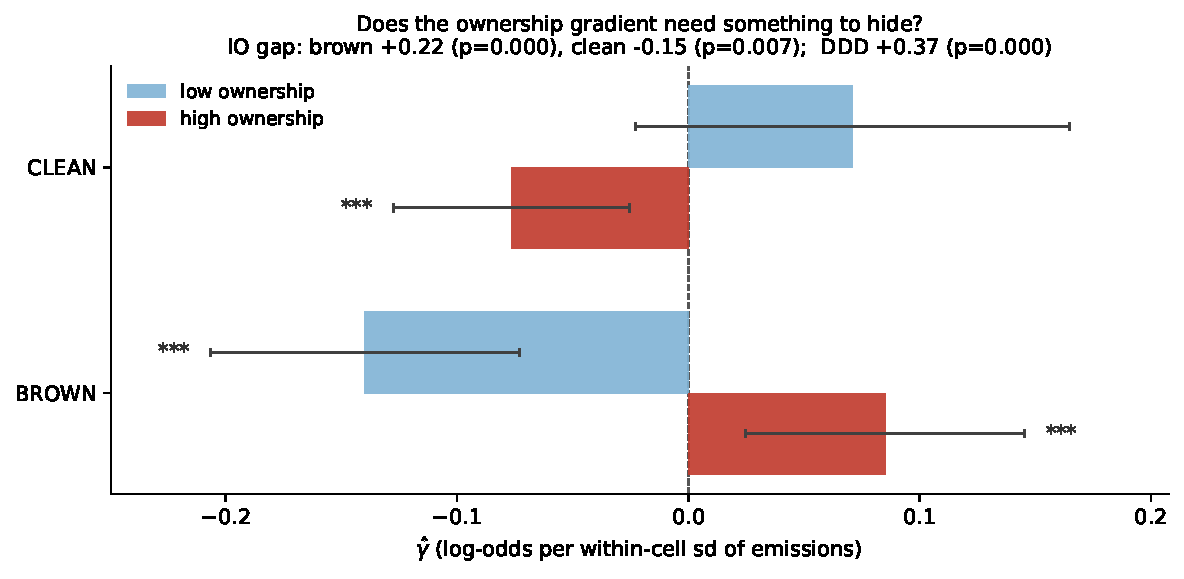
\includegraphics[width=0.95\linewidth]{figs/gamma_audience_x_brown_tilt_test.pdf}
    \caption{\textbf{The ownership gradient appears only where there is something to hide.} Estimated $\hat\gamma$ in each of four cells defined by within-sector institutional ownership (above or below the sector median) and industry carbon intensity revealed by disclosing firms (above or below the sample median), with 95\% confidence intervals. Positive $\hat\gamma$ indicates strategic silence. The specification includes sector, year and ownership fixed effects and allows the size slope to differ across cells. Emissions are standardized within cell, so $\hat\gamma$ is in log-odds per standard deviation of emissions present in that group.}
    \label{fig:gamma_brown}
\end{figure}

Figure~\ref{fig:gamma_brown} reports the four estimates, and the pattern is the one the audience mechanism predicts and the disclosure-capacity account does not. Among brown firms, selection severity rises from $-0.140^{***}$ where ownership is dispersed to $+0.085^{***}$ where it is concentrated, a gap of $+0.225$ ($p<0.001$). Among clean firms the gradient is absent and if anything runs the other way: $+0.071$ (insignificant) at low ownership against $-0.076^{***}$ at high, a gap of $-0.147$ ($p=0.007$). The triple difference that constitutes the test, i.e. the difference between the two gaps, is $+0.372$ (s.e.\ $0.070$, $p<0.001$).\footnote{Replacing industry carbon intensity with firm-level PP\&E intensity, a reported measure of physical-capital heaviness that splits firms \emph{within} industry rather than across, gives a triple difference of $+0.285$ (s.e.\ $0.071$, $p<0.001$). That proxy is, however, sensitive to the standardization convention in a way industry carbon intensity is not: under within-sector standardization it falls to $+0.115$ ($p=0.23$), and we report industry carbon intensity as the primary measure for that reason. Table~\ref{tab:gamma_brown_robustness} in Appendix~\ref{app:robustness} reports every cell estimate and contrast under both proxies and both standardization conventions. Third-party vendor carbon intensity is unusable in this design, because vendor coverage is itself a function of disclosure and conditioning on a non-missing estimate therefore selects on the outcome.}

The key feature of the evidence is that the ownership gradient changes sign rather than merely shrinking. Size, liquidity, index membership, and reporting capacity all predict an ownership gradient of the same sign regardless of whether firms have high emissions. None predicts that the gradient disappears or reverses among firms with little carbon to conceal. The four cells also trace Proposition~\ref{prop:gamma} directly. Effective severity $\gamma_{\text{eff}} = (\beta + c_1 - b)/\lambda$ is positive in the single cell where scrutiny has something to bite on -- concentrated ownership together with high emissions -- and zero or negative in the other three, where the transparency benefit $b$ dominates instead. Both of the model's opposing forces are therefore visible in one cross-section, and they appear where the theory says they should rather than being assumed.

Overall, we find that where firms face an audience, high emitters strategically hide and selection bites. Where ownership is dispersed and no one is systematically watching, the disclosure decision is dominated by alternative motives -- signaling to attract capital, idiosyncratic owner preferences, measurement capacity -- and selection weakens and turns negative.


\subsection{The emergence of an audience}
\label{subsec:regime}

Section~\ref{subsec:boundary} showed that selection severity depends on the audience in the cross-section: $\gamma$ is positive where institutional ownership is concentrated and turns negative where it is dispersed. This subsection asks whether the same dependence appears over time -- whether an audience that reads the carbon-disclosure decision as informative \emph{formed} during the sample, and if so when. The evidence here is behavioural: a year-by-year selection-severity trajectory estimated from the propensity model alone. Its price counterpart -- the market's reaction when a disclosure mandate became likely in March 2022 -- is a returns test, and is reported with the other pricing evidence in Section~\ref{subsec:sec_event}; we read the two as parallel rather than as a causal chain. A third exercise bearing on the same question, the within-firm transition difference-in-differences, is reported with the transparency premium in Section~\ref{subsec:premium}; its cohort pattern turns out to be sector composition, and we do not rely on it here.

We estimate the selection severity year by year from the propensity model alone by interacting emissions with year indicators, and ask when it intensifies. Figure~\ref{fig:gamma_by_year} reports $\hat\gamma_t$ scaled by the within-year standard deviation of emissions, so each point is the log-odds change from a one-standard-deviation move in emissions in that year.

\begin{figure}[htbp]
    \centering
    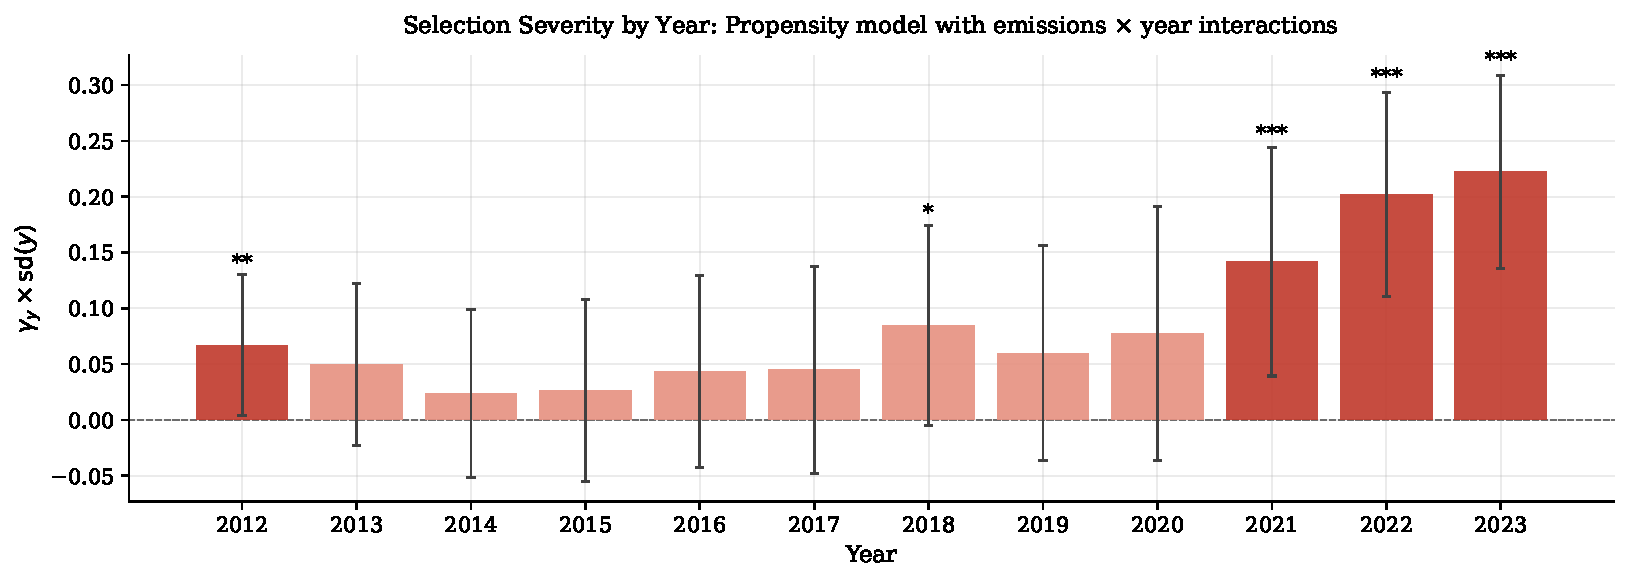
\includegraphics[width=0.95\linewidth]{figs/gamma_by_year_tilt_test.pdf}
    \caption{\textbf{Selection severity by year.} Estimated $\hat\gamma_t$ from a propensity model with emissions $\times$ year interactions, scaled by the within-year standard deviation of emissions, with 95\% confidence intervals. Positive $\hat\gamma_t$ indicates strategic silence: higher emitters are less likely to disclose. The specification includes size, sector, and year fixed effects; 2012 is the first year of Trucost coverage. Stars denote significance at the 10\%, 5\%, and 1\% levels.}
    \label{fig:gamma_by_year}
\end{figure}

The trajectory is flat and then steep. From 2013 through 2020, $\hat\gamma_t$ is small and, with the single exception of 2018 ($+0.085^{*}$), statistically indistinguishable from zero: over most of the 2010s we cannot reject that disclosure is unrelated to the emissions level once size, sector, and year are controlled for. The final three years break sharply from this: $\hat\gamma_{2021} = +0.142^{***}$, $\hat\gamma_{2022} = +0.202^{***}$, and $\hat\gamma_{2023} = +0.222^{***}$, each significant at the 1\% level and each larger than any earlier estimate.\footnote{The first sample year is an exception to the flat early pattern ($\hat\gamma_{2012} = +0.067^{**}$). We set it aside: 2012 is the first year of Trucost coverage, when the disclosing sample is both smallest and least representative, and the estimate is not part of any monotone pattern with adjacent years.} By the end of the sample, a one-standard-deviation increase in emissions moves the log-odds of disclosure by more than two and a half times what it did in the largest pre-2021 year.

The intensification is not a structural break. It is natural to ask whether these three years reflect a discrete regime change at an identifiable date, and we tested for one with a cutoff-sensitivity (sup-Wald) scan over candidate split years, following \citet{andrews1993tests} with 15\% trimming. The test rejects the null of constant $\gamma$ decisively -- the maximized Wald statistic of $21.3$ exceeds the 1\% critical value -- but it does \emph{not} locate a break, and the reason is visible in the shape of the scan rather than in its argmax. The Wald statistic rises monotonically across every candidate cutoff ($0.4$ at 2014, $5.0$ at 2016, $10.2$ at 2018, $16.1$ at 2020, $21.3$ at 2022) and is still rising when the trimming window ends. A genuine break produces a Wald surface that peaks at the break date and declines on either side; a surface that is monotone to the boundary is the signature of a continuous change, or of a break at or beyond the edge of the admissible range.

The argmax is accordingly an artifact of where the scan stops rather than a feature of the data. Dropping 2023 and re-running moves the last admissible cutoff from 2022 to 2021, and the argmax follows it exactly, to 2021, while the surface remains monotone. Any date we reported from this procedure would track our sample end rather than any economic event, so we report none. We note also that the conventional $p$-values from such a scan are not interpretable at the argmax, since searching over cutoffs invalidates the $\chi^2$ null -- which is precisely what the \citet{andrews1993tests} critical values correct for, and why we use the test only to reject constancy.

The two objects agree, and they support a claim about a period rather than a date: strategic silence is weak and statistically absent through 2020 and intensifies sharply over 2021--2023. The monotone Wald surface is exactly what this trajectory implies mechanically -- pushing the cutoff later isolates a progressively purer post-period of high-severity years, so the pre/post contrast keeps growing -- and it is why the scan cannot separate a late break from a late-concentrated trend. The intensification coincides with a broad shift in U.S. climate scrutiny: the surge in sustainable investment, the re-engagement with Paris, and the build-up to the SEC's proposed climate-disclosure rule. We do \emph{not} attribute it to any single rule. The annual test cannot resolve a specific date within 2021--2023, and it is silent on the March 2022 SEC proposal, which we examine as a separate, higher-frequency test below.

% ============================================================
\section{Pricing}
\label{sec:pricing}\label{subsec:return_spec}

This section turns from the disclosure decision to its price. Having established where strategic silence operates, we ask what the market pays for it: whether the emissions \emph{level} is priced (Section~\ref{subsec:bk}), whether the disclosure \emph{decision} itself carries a premium (Section~\ref{subsec:premium}), and how prices moved when a disclosure mandate became likely (Section~\ref{subsec:sec_event}).

Throughout the pricing tests we estimate panel regressions of monthly firm returns, in percentage points, on a measure of recovered emissions, with a common set of firm-level controls. The controls follow \citet{bolton2021investors} (BK hereafter): market beta, momentum (twelve-month, skipping the most recent month), twelve-month return volatility, log market capitalization, investment-to-assets, the Herfindahl index of industry concentration, leverage, log property, plant and equipment, return on equity, log book-to-market, sales growth, and earnings-per-share growth. Every right-hand-side variable, controls and emissions alike, is lagged one month relative
to the return it explains, winsorized within the cross-section, and standardized to unit variance within each month; coefficients are therefore read as the return, in percentage points per month, associated with a one-standard-deviation move in the
regressor, holding the others fixed. Standardizing within month rather than pooling prevents secular growth in emissions or in any control from loading on the cross-sectional slope, and lagging ensures the regressors are in the investor's information set at the start of the return month. Standard errors are clustered at the firm level throughout, which accommodates arbitrary within-firm serial correlation in returns over the twelve-year panel.

We report each result under a progression of fixed-effect structures, so that a coefficient can be read against successively more demanding sources of identifying variation. The baseline includes time (year-month) and industry fixed effects, so
that emissions are compared across firms within the same industry and month. Dropping the industry effects, leaving time effects alone, asks whether the relation survives without within-industry conditioning; adding firm fixed effects in place of industry effects, so that identification comes only from within-firm variation over time, asks whether it is a cross-firm or a within-firm signal. Reading a coefficient across these three columns is informative in itself: stability from the first to the second locates the signal within or across industries, and a change from the first to the third separates cross-firm from within-firm pricing.
\subsection{Diagnostic: the levels premium}
\label{subsec:bk}

Before the affirmative results, we ask what the recovered emissions do to the cross-sectional carbon premium as it is usually estimated -- on the level of
emissions -- and use the exercise to establish that the selection correction is not mechanically driving anything downstream. Table~\ref{tab:returns_main} regresses monthly returns on standardized Scope~1 emissions across three measures (observed or
vendor, MNAR-corrected, and MAR-imputed) and three samples (firms that report, firms that report or are vendor-covered, and the full universe).

\begin{table}[htbp]
\footnotesize\centering
\caption{\textbf{Carbon Emissions and Stock Returns.}
Panel regressions of monthly stock returns on standardized Scope~1 CO$_2$ emissions.
All specifications include firm characteristics, time fixed effects, and industry fixed effects,
following \citet{bolton2021investors}.Columns~(1) and~(2) compare observed and corrected emissions on subsamples with available data. Column~(3) uses corrected emissions on the full Compustat universe.
Panel~B uses MNAR-corrected emissions. Panel~C uses MAR-imputed emissions: outcome model only. The comparison between Panels~B and~C isolates the contribution of the selection correction. Standard errors are clustered at the firm level.}
\label{tab:returns_main}
\begin{tabular}{lccc}
\toprule
 & (1) & (2) & (3) \\
 & Disclosed & Combined & Full Sample \\
\midrule
\textit{Panel A: Observed / vendor emissions} & & & \\[2pt]
Scope~1 Emissions & 0.018 & 0.040$^{**}$ & -- \\
 & (0.028) & (0.020) & \\

\textit{Panel B: MNAR-corrected emissions} & & & \\[2pt]
Scope~1 Emissions & -0.003 & 0.004 & -0.001 \\
 & (0.022) & (0.024) & (0.025) \\

\textit{Panel C: MAR-imputed emissions} & & & \\[2pt]
Scope~1 Emissions & -0.002 & 0.010 & 0.001 \\
 & (0.019) & (0.020) & (0.023) \\
\midrule
Controls & Yes & Yes & Yes \\
Time FE & Yes & Yes & Yes \\
Industry FE & Yes & Yes & Yes \\
Obs (Panel A) & 47,601 & 124,130 & -- \\
Obs (Panels B--C) & 47,601 & 124,130 & 209,761 \\
\bottomrule
\end{tabular}
\begin{flushleft}\footnotesize
\textit{Notes:} Returns are in percentage points.
Emissions are standardized within month on the relevant subsample. Column~(3) has no Panel~A row because never-disclosing firms have no
reported or vendor-estimated value by construction.
Significance: $^{***}p<0.01$, $^{**}p<0.05$, $^{*}p<0.10$.
\end{flushleft}
\end{table}

Panel~A, which uses observed emissions throughout, reconciles the two findings the literature has struggled to square, and it does so without any recourse to imputation. Among firms that report their emissions directly, column~(1), the premium is $0.018$ percentage points per month per standard deviation and is statistically indistinguishable from zero -- the \citet{aswani2024carbon} null. Adding the firms whose emissions are vendor-estimated rather than reported, column~(2), raises the coefficient to $0.040$ and renders it significant at five percent -- the \citet{bolton2021investors} premium. The two results are not in conflict; they are the same regression run on two nested samples, and the premium is exactly the increment contributed by the vendor-estimated observations. Because both columns use
only observed values, neither is subject to the attenuation that afflicts any regression on imputed data, so this contrast is the cleanest statement the paper can make about the levels premium: it is present when vendor estimates are included and
absent when they are not.

Panels~B and~C carry that logic into the corrected measures, and here the reading must be more guarded. Replacing observed emissions with the MNAR-corrected values collapses every coefficient toward zero: the vendor-inclusive premium of column~(2) falls from $0.040$ to $0.004$, and no cell in the panel approaches significance, including on the full universe of column~(3), where the measure is defined
for the never-disclosing majority for the first time. Panel~C repeats the exercise with a plain missing-at-random fill and returns almost the same numbers -- $-0.002$, $0.010$, and $0.001$ against Panel~B's $-0.003$, $0.004$, and $-0.001$. That near-identity is the diagnostic these two panels exist to provide: the exponential tilt, which is the only thing that distinguishes the MNAR correction from the MAR
baseline, moves no cross-sectional return coefficient by as much as a standard error. Whatever the pricing results of the following subsections rest on, they do not rest on the tilting step, which neither creates nor removes a levels premium. The two sides of the paper use the correction differently. The tilt's payoff is in measurement: the upward revision of aggregate emissions and carbon damages in Section~\ref{subsec:aggregate} is entirely a property of the recovered upper-tail mass the tilt supplies, and there Panels~B and~C would diverge sharply. The pricing tests draw something else from the model -- the recovered \emph{sample}, which defines emissions for the never-disclosing majority for the first time, and the selection-severity pattern $\hat\gamma$ across audiences -- neither of which is the tilt magnitude. That the tilt moves no return coefficient is therefore a robustness feature, not a puzzle: the pricing conclusions survive whatever residual uncertainty attaches to the size of the correction.

The fall of the premium from Panel~A to Panel~B is not by itself decisive. Imputation introduces measurement error, which attenuates coefficients toward zero, so the drop from $0.040$ to $0.004$ is consistent both with a vendor premium that is not a robust feature of firm emissions and with mechanical attenuation from a noisier regressor. The comparison
that does not suffer this ambiguity is the one within Panel~A, between firm-reported and vendor-inclusive observed emissions, and it is on that comparison that we lean: the levels premium is a property of the vendor-estimated values, not of firm-reported
emissions, precisely as \citet{aswani2024carbon} argues. This conclusion sits alongside the vendor-estimate placebo in the event study of Section~\ref{subsec:sec_event}, where Trucost values load significantly on a date with no climate news at all -- a horizon at which the recovered emissions do not -- indicating a component of the vendor measure that moves with prices for reasons unrelated to climate policy. The affirmative pricing result of the paper is therefore not a claim about the level of
emissions at all; it concerns the disclosure decision, to which we turn in the next section.

\paragraph{Intensity, unlike levels, carries a signal in clean data.}
Scaling emissions by output, as \citet{aswani2024carbon} advocates, changes the
picture in a way that is instructive precisely because it differs from the levels result. Table~\ref{tab:returns_intensity} regresses returns on log Scope~1 intensity, and column~(1), which restricts to firms that report their emissions directly, returns $-0.166$ percentage points per month per standard deviation, significant at five
percent. This is the same firm-reported sample on which the emissions \emph{level} carried no premium at all ($0.018$, insignificant, Table~\ref{tab:returns_main}), so the two tables together draw a clean line: the level is not priced in disclosed data, but intensity is. The relation is not a property of vendor estimation. Adding the vendor-estimated firms in column~(2) leaves it essentially unchanged at $-0.141$, a coefficient statistically indistinguishable from the firm-reported one, and the selection correction extends it to the full Compustat universe in column~(3) at $-0.246$. Where the positive levels premium of the previous table appeared only once vendor values were included -- the \citet{aswani2024carbon} critique -- the negative
intensity relation is already present among firms that report, and the recovered data carry it to the rest of the cross-section.

The sign warrants the same caution we gave it before: higher-intensity firms earn \emph{lower} returns, which is the opposite of a carbon-risk premium and a statement about realized returns over a decade, 2013--2023, in which low-carbon firms outperformed. The natural reading is that of \citet{pastor2025green}: an unanticipated rise in climate concern lifted the prices of low-intensity firms in-sample, a realized outcome rather than a compensating expected return. We report the intensity relation not as a structural premium but because it completes the measurement contrast -- the level carries nothing robust, intensity carries a realized green-outperformance signal, and neither is what the disclosure premium of Section~\ref{subsec:premium} captures, which is orthogonal to both. Two features of the table reinforce that it is the measured relation rather than the correction doing the work: the column~(1) coefficient is identical across the three panels because, for disclosing firms, the corrected and imputed measures simply return the reported value; and the MNAR and MAR panels agree to the third decimal ($-0.192$ against $-0.190$, $-0.246$ against $-0.246$), so the exponential tilt neither manufactures the intensity relation nor inflates it.

\subsection{The transparency premium}
\label{subsec:premium}

The levels premium having failed to survive either measurement or sample extension,
we turn to the disclosure decision itself. Table~\ref{tab:returns_disc_premium}
regresses monthly returns on an indicator for whether a firm voluntarily discloses its Scope~1 emissions, on the full sample and with the same controls, time,
and industry fixed effects as before. Column~(1) estimates a disclosure premium of $0.242$ percentage points per month, with a firm-clustered standard error of $0.057$, a $t$-statistic above four. The magnitude is economically substantial: nearly three
percentage points per year separate a disclosing firm from an observably comparable firm in the same industry and month that stays silent. Where the level of emissions was priced weakly and only in vendor-inclusive samples, the \emph{act} of disclosure
carries a premium an order of magnitude more precisely estimated.

\begin{table}[htbp]
\footnotesize\centering
\caption{\textbf{Disclosure Premium: Does MNAR Correction Absorb the Return to Disclosure?}
Panel regressions on the full Compustat sample.
Column~(1) estimates the return premium to voluntary disclosure.
Column~(2) adds MNAR-corrected emissions.
Column~(3) repeats with MAR-imputed emissions.
Column~(4) reports MNAR emissions without the disclosure dummy.
Standard errors clustered at the firm level.}
\label{tab:returns_disc_premium}
\begin{tabular}{lcccc}
\toprule
 & (1) & (2) & (3) & (4) \\
 & Disc Only & +MNAR & +MAR & MNAR Only \\
\midrule
Disclosed & 0.242$^{***}$ & 0.242$^{***}$ & 0.242$^{***}$ & -- \\
 & (0.057) & (0.057) & (0.057) & \\

Scope~1 Emissions & -- & -0.001 & -0.001 & -0.001 \\
 & & (0.025) & (0.023) & (0.025) \\
\midrule
Controls    & Yes & Yes & Yes & Yes \\
Time FE     & Yes & Yes & Yes & Yes \\
Industry FE & Yes & Yes & Yes & Yes \\
Observations & 209,761 & 209,761 & 209,761 & 209,761 \\
$R^2$ & 0.208 & 0.208 & 0.208 & 0.208 \\
\bottomrule
\end{tabular}
\begin{flushleft}\footnotesize
\textit{Notes:} Stability of the Disclosed coefficient from~(1) to~(2) indicates
the market prices the disclosure decision, not the emissions level,
consistent with \citet{verrecchia1983discretionary} and \citet{milgrom1981good}. Significance: $^{***}p<0.01$, $^{**}p<0.05$, $^{*}p<0.10$.
\end{flushleft}
\end{table}

The next two columns establish that this premium and the emissions level are orthogonal in their return implications. Adding MNAR-corrected emissions to the
regression, column~(2), leaves the disclosure coefficient at $0.242$ -- unchanged to
three decimal places -- while the emissions coefficient is itself $-0.001$ and insignificant. Substituting the MAR-imputed measure, column~(3), reproduces the same pair of numbers, and dropping the disclosure indicator to leave emissions alone,
column~(4), still returns $-0.001$. The $R^2$ is $0.208$ in every column: conditional on the disclosure decision and the controls, the level of emissions explains no additional variation in the cross-section of returns, and the disclosure premium is undisturbed by whether, and how, emissions are added to the regression. Two objects that the disclosing-sample literature could only observe jointly are here separated, and only one of them is priced. What the market compensates is the decision to
reveal, not the quantity revealed.

The premium is a cross-sectional differential, not a causal effect. The regression conditions on industry, month, and the standard return predictors, but not on firm identity, so it compares disclosing firm-months to non-disclosing firm-months. Firms that disclose differ from firms that do not along dimensions no set of observables fully captures -- governance, investor base,
anticipated scrutiny -- and any of these could carry an independent return implication. We therefore do not read the $0.242$ as the causal effect of a firm's
flipping from silence to disclosure; it is the return differential associated with the disclosure decision, conditional on observables, and it may reflect a risk premium, a slow price adjustment, or selection on characteristics we do not measure. The claim that survives all of these readings is the one the table was built to make, and it is enough for the argument: whatever the disclosure indicator captures, it is not the level of emissions, which enters at zero and moves neither the premium nor the fit. The within-firm counterpart to this comparison follows a firm across its own transition into disclosure, and it is there, rather than in the cross-section, that a causal reading can be tested. Of our sample, $680$ firms move from non-disclosure to voluntary disclosure over 2012--2023. For each we define event time $e_{it} = t - t^{\ast}_i$ around the first-disclosure year $t^{\ast}_i$ and estimate, over windows $e_{it} \in [-2,+2]$, $[-2,+4]$, $[-4,+4]$,
\begin{equation}
\label{eq:did}
r_{it} = \tau\,(\mathrm{High}_i \times \mathrm{Post}_{it})
       + \phi\,\mathrm{High}_i + \delta\,\mathrm{Post}_{it}
       + \psi' \mathbf{x}_{it} + \mu_{j(i)} + \lambda_t + \varepsilon_{it},
\end{equation}
where $\mathrm{Post}_{it} = \mathbf{1}\{e_{it} \geq 0\}$; $\mathrm{High}_i$ is a top-quartile emitter, assigned on the recovered measure at $t-1$ and on the disclosed value at $t=0$, the two agreeing on $89\%$ of firms; $\mathbf{x}_{it}$ is the control vector of Section~\ref{subsec:return_spec}; and $\mu_{j(i)}$, $\lambda_t$ are industry and calendar-month fixed effects, with standard errors clustered by firm.

The coefficient that speaks to the premium is $\delta$, the within-firm change in returns around disclosure. It is negative in every window and specification -- across both treatment definitions, within firm, and under sector-by-year fixed effects -- ranging from $-0.12$ to $-0.52$, estimated less precisely as the fixed effects saturate but never changing sign (Table~\ref{tab:returns_did_post_iy}). A firm's returns are, if anything, lower after it begins disclosing than before. That is the sign the cross-sectional premium lacks, and the two are not the same object: $\delta$ compares a firm with itself, while the $+0.242$ compares different firms. Together they indicate that the premium reflects the characteristics of firms that choose to disclose rather than a causal return to the act -- the act itself, if anything, lowers returns in the way a resolution of uncertainty should. This is why we decline to read the $0.242$ causally.

A natural next question is whether the within-firm change depends on \emph{how much} carbon a firm reveals, which is the interaction $\tau$. The model predicts that it should: by Lemma~\ref{lemma:indiv_best_resp} the transition return is $-\beta\,(y_i - \mu_{ND})$, so a firm revealing worse-than-pooled emissions should fall relative to one revealing better. Pooled, $\hat\tau$ is positive, $+0.45$ to $+0.58$; split by first-disclosure cohort it appears to reverse, from $-0.66$ in 2017--2019 to $+1.20$ in 2020--2023 (Table~\ref{tab:returns_did_cohort_year}). That reversal does not survive the check its construction invites. High-emitting transition firms concentrate in Energy, Materials, Utilities, and Industrials -- the sectors that rallied over 2021--2023 as commodity prices and inflation rose -- so the level-based $\mathrm{High}$ indicator is close to a sector indicator, and the post-2020 window loads that sector return onto it. Sector-by-year fixed effects, which absorb any industry-wide annual return, collapse the 2020--2023 coefficient from $+1.20$ to $+0.27$ and remove its significance (Table~\ref{tab:returns_did_industry_year}); dropping Energy and Materials alone, some thirty firms, removes three-quarters of it. Redefining treatment as the disclosure \emph{surprise} -- $\log(\text{disclosed}_{t=0}) - \log(\text{predicted}_{t-1})$, nearly orthogonal to sector by construction and empirically so, since a sector-only regression explains two percent of its variance against forty-nine percent of the level -- returns a null: $\hat\tau = -0.13$ over $[-2,+2]$ with a $95\%$ confidence interval of $[-0.61,\,+0.35]$ (Table~\ref{tab:returns_did_surprise}). That interval excludes the $+1.20$ the level-based design produced, so the null is informative about an effect of that magnitude rather than merely underpowered, though it is wide enough that a small repricing cannot be ruled out. The episode carries a caution beyond this paper: a treatment indicator built on the level of emissions is close to a sector indicator, so any event-time or difference-in-differences design that sorts firms on emissions levels inherits whatever their sectors did over the window.

Read through the model, this null is the third consistent sign of one fact. The selection severity decomposes as $\gamma = (\beta + c_1)/\lambda$ in \eqref{eq:disclosure_threshold}, with $\beta$ the market's price impact on revealed emissions and $c_1$ the private cost of revelation; the transition return $-\beta(y - \mu_{ND})$ is governed by $\beta$ alone, so a null on the surprise says $\beta$ is small in this sample. Two other results say the same: the emissions level is unpriced among disclosers (Table~\ref{tab:returns_main}, column~1), and intensity carries a negative loading we read as realized green outperformance rather than a risk premium (Section~\ref{subsec:bk}). With $\beta$ small, the selection severity we estimate is essentially the $c_1$ channel -- the private and regulatory cost of revelation, not a standing carbon-risk premium -- which is also what its intensification over 2021--2023 (Section~\ref{subsec:regime}) reflects. The two-channel decomposition survives; the data tell us which channel is operative.

\subsection{The SEC climate-disclosure proposal}
\label{subsec:sec_event}

On 21 March 2022 the SEC proposed a rule that would have required registrants to report greenhouse-gas emissions. For firms already disclosing, the proposal threatened little; for firms that had not, it raised the prospect that emissions they had kept private would become public. If the market forms a view about what those firms are hiding -- the suspicion discount that Section~\ref{sec:theory} makes the economic content of silence -- then the announcement should move their prices in proportion to the emissions the market infers, and our recovered measure should predict the reaction. We therefore restrict attention to the $3{,}190$ firms that had not voluntarily disclosed as of the year before the event, the population for which no firm-reported figure was available when the proposal landed and for which our measure is consequently imputed rather than observed.\footnote{A subset of these firms carry a Trucost vendor estimate; we retain them because they permit the horse race reported below, and because the relevant margin for the event is the absence of a \emph{firm-reported} number, not the absence of vendor coverage. Non-disclosure is measured in the pre-event year rather than over the whole sample, so the group comprises firms silent at the time of the announcement rather than firms that never disclose at any point.} Abnormal returns are computed from a market model estimated over days $[-250,-30]$, and cumulative abnormal returns are regressed on log recovered emissions measured in the pre-event year, with sector fixed effects, a log-assets control, and heteroskedasticity-robust standard errors.


\begin{table}[htbp]
\footnotesize\centering
\caption{\textbf{Market reaction to the SEC climate-disclosure proposal.}
Cumulative abnormal returns around the proposal of 21 March 2022, regressed
on log recovered Scope~1 emissions measured in the pre-event year. The sample
is firms that had not voluntarily disclosed as of that year, for whom the
emissions measure is imputed rather than reported; abnormal returns come from
a market model estimated over days $[-250,-30]$. The placebo columns repeat
the identical construction on the same calendar date in 2019, a date with no
climate-policy news, rebuilding the sample from firms not disclosing as of
2018. Sector fixed effects throughout; heteroskedasticity-robust standard
errors in parentheses.}
\label{tab:returns_event_study}
\begin{tabular}{lcccccc}
\toprule
 & \multicolumn{3}{c}{SEC proposal (2022-03-21)} & \multicolumn{3}{c}{Placebo (2019-03-21)} \\
\cmidrule(lr){2-4}\cmidrule(lr){5-7}
 & $[-1,+1]$ & $[-5,+5]$ & $[-30,+30]$ & $[-1,+1]$ & $[-5,+5]$ & $[-30,+30]$ \\
\midrule
MNAR emissions & -0.0051$^{***}$ & -0.0091$^{***}$ & 0.0025 & 0.0009 & -0.0010 & -0.0015 \\
 & (0.0009) & (0.0018) & (0.0051) & (0.0007) & (0.0015) & (0.0035) \\
Log assets & -0.0003 & 0.0076$^{***}$ & -0.0226$^{***}$ & -0.0011 & -0.0009 & -0.0121$^{**}$ \\
 & (0.0013) & (0.0023) & (0.0075) & (0.0009) & (0.0019) & (0.0047) \\
\midrule
Sector fixed effects & Yes & Yes & Yes & Yes & Yes & Yes \\
Observations & 3,190 & 3,190 & 3,190 & 3,061 & 3,061 & 3,061 \\
$R^2$ & 0.033 & 0.037 & 0.038 & 0.017 & 0.010 & 0.012 \\
\bottomrule
\end{tabular}
\begin{flushleft}\footnotesize
\textit{Notes:} Coefficients are per one-log-unit (roughly $2.7$-fold)
increase in recovered emissions; CARs are in decimal returns, so $-0.0051$
is $-0.51$ percentage points. A multi-date version of the placebo, comparing
the event coefficient with the distribution over the twenty-first of every
month in the sample, is reported in Table~\ref{tab:returns_event_placebo_dist}.
Significance: $^{***}p<0.01$, $^{**}p<0.05$, $^{*}p<0.10$.
\end{flushleft}
\end{table}

The reaction is negative, immediate, and confined to tight windows (Table~\ref{tab:returns_event_study}, columns~1--3; columns~4--6 repeat the exercise on a placebo date discussed below). Over the three-day window a one-log-unit increase in recovered emissions -- roughly a $2.7$-fold increase -- is associated with a cumulative abnormal return lower by $0.51$ percentage points; over eleven days the figure is $0.91$ percentage points. Over the two-month window the coefficient is $+0.25$ percentage points and indistinguishable from zero. We read the wide-window null as the absence of evidence for persistent repricing rather than as a contradiction of the short-window result: the sixty-day window admits two months of unrelated news, and event studies have most power precisely where the announcement effect is concentrated. What the short windows establish is that on the days surrounding the proposal, firms our procedure identifies as high emitters -- firms that had told the market nothing -- fell relative to otherwise similar firms in the same sector and of the same size.

That the measure is predictive at all is the substantive point, since these are firms whose emissions the market could not read off any disclosure. The variation doing the work is narrow. Because the regression conditions on sector and on log assets, and because the outcome model predicts emissions from size, industry, and oil-price exposure, what remains after those controls is variation in narrower industry composition and in predetermined physical-capital intensity. The finding is thus that the market's reaction to a prospective disclosure mandate lines up with the emissions ordering our model implies within sector and size, which validates the recovered measure without being independent of the inputs that construct it.

Columns~4--6 of Table~\ref{tab:returns_event_study} repeat the identical construction on the same calendar date in 2019, a day with no climate-policy news, rebuilding the sample from firms not disclosing as of 2018. Nothing appears. But a single placebo date establishes only that one other day was quiet, which is weak evidence that the event day was unusual. We therefore re-estimate the regression on the twenty-first of every month in the sample, $131$ dates in all, rebuilding the non-disclosing sample and the recovered emissions measure date by date, and compare the event coefficient with the resulting distribution (Table~\ref{tab:returns_event_placebo_dist} and Figure~\ref{fig:event_placebo_dist}). 

The event coefficient sits in the far left tail. At both the three- and eleven-day windows exactly one of the $131$ placebo dates produces a more negative coefficient, an empirical $p$-value of $0.015$, and the event lies about three placebo standard deviations below a placebo distribution that is itself centred on zero -- its means are $0.0000$, $0.0002$, and $-0.0001$ across the three windows, so the estimator carries no mechanical tendency toward negative coefficients. The number of placebo dates matters for how this should be read: with $131$ of them the smallest attainable $p$-value is $0.008$, so $0.015$ is a genuine rejection with room beneath it rather than an artifact of too few comparisons.\footnote{Restricting the placebos to every 21 March, which holds the calendar date exactly fixed at the cost of only ten comparisons, the event coefficient is more negative than \emph{all} of them; the resulting $p$-value of $0.091$ is that design's floor rather than a weaker result. The two schemes trade seasonal control against power, and they agree.} Excluding every month of 2020 and 2021 as confounded -- the COVID drawdown and the period following U.S.\ re-entry to the Paris agreement -- drops twenty-four dates and moves the figure only to $0.019$; the single placebo that exceeds the event falls outside those years, so the result rests on neither. The two-month window, by contrast, is indistinguishable from placebo ($p = 0.614$), and its placebo distribution is three times as dispersed.

One coincidence in the event window deserves comment. The Federal Reserve raised rates on 16 March 2022, the first hike of that cycle, which falls three trading days before the SEC announcement and therefore inside the eleven-day window but outside the three-day one. Because recovered emissions correlate with capital intensity, a differential response to monetary tightening could in principle load on the same regressor. The tight window settles the question: it excludes the FOMC date entirely and returns the same randomization $p$-value as the wider one ($0.015$ in both), so the result does not depend on the days containing the rate decision. We note in addition that the Federal Open Market Committee meets eight times a year, so a $\pm 5$-day window spans a meeting roughly a quarter of the time and many placebo dates are similarly affected; windows containing monetary news are part of the null distribution rather than a departure from it.

A sharper version of the test narrows the sample further. Roughly half the firms above carry a Trucost vendor estimate -- a figure the market could have bought even though the firm itself disclosed nothing -- so for them one might argue the announcement was priced off the vendor number rather than off anything our procedure uniquely recovers. We therefore re-estimate on the $1{,}648$ firms that Trucost does
not cover at all, for whom no emissions figure of any kind was available. The reaction survives: $-0.44$ percentage points over three days and $-0.75$ over eleven, both significant at one percent, against $-0.51$ and $-0.91$ in the full sample (Table \ref{tab:returns_event_study_none}). The
coefficients are some fifteen percent smaller and their standard errors larger, as one expects when the sample halves and the firms that remain are smaller and less liquid, but the two sets of estimates are within sampling error of each other, and the placebo stays clean at every horizon. For this group the recovered emissions are the only emissions figure in existence, so the market's reaction cannot be
attributed to a vendor estimate read in their place.\footnote{The Trucost horse race
of Table~\ref{tab:returns_event_study_trucost_vs_mnar_main} necessarily runs on the complementary subsample, since it requires a vendor estimate to exist. The two
exercises are therefore not nested: one asks whether the recovered measure adds information where a vendor figure is available, the other whether it works where none is.}


One qualification applies to the inference itself. The placebo coefficients are not independent draws, since the same firms recur at every date and adjacent dates share most of their market-model estimation window, so the effective number of comparisons is below $131$ and the empirical $p$-value is correspondingly optimistic. The eleven-day event windows themselves do not overlap at monthly spacing, so the outcome variable is clean; it is the sample and the estimation window that induce the dependence. We report the figure as strong corroboration rather than as an exact size.

\begin{figure}[htbp]
    \centering
    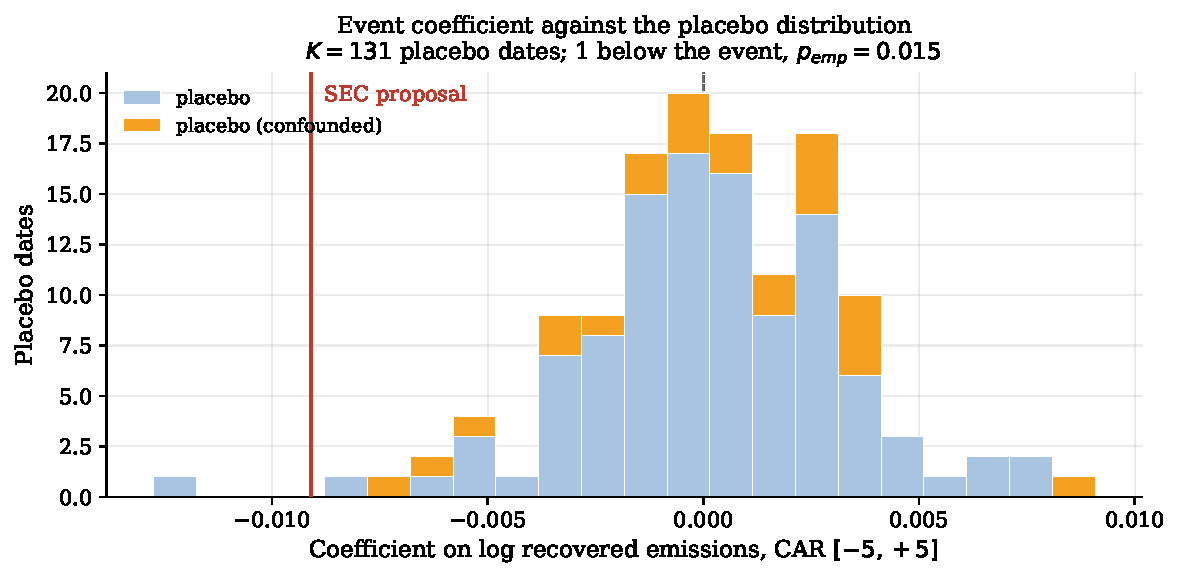
\includegraphics[width=0.85\linewidth]{figs/returns_event_placebo_dist.pdf}
    \caption{\textbf{The event coefficient against the placebo distribution.} Each of the $131$ placebo observations is the coefficient on log recovered emissions from the event-study regression of Table~\ref{tab:returns_event_study}, re-estimated on the twenty-first of a non-event month with the sample and the emissions measure rebuilt for that date. The vertical line marks the SEC-proposal coefficient for the $[-5,+5]$ window; exactly one placebo lies to its left. Shading marks the twenty-four dates in 2020 and 2021 flagged as confounded by the COVID drawdown and by U.S.\ re-entry to the Paris agreement; they are retained here and excluded only from the $p_{\text{clean}}$ column of Table~\ref{tab:returns_event_placebo_dist}.}
    \label{fig:event_placebo_dist}
\end{figure}

The comparison with vendor estimates is more nuanced than a simple contrast between a working measure and a broken one. Restricting to the $1{,}542$ firms that carry both a Trucost estimate and our recovered value, and entering the two together, the recovered emissions retain an independent effect on the event date: $-0.0050$ over three days and $-0.0103$ over eleven, both significant at one percent. Trucost is not uninformative alongside them -- it enters at $-0.0043$ and $-0.0047$ in the same specifications -- and we would not expect otherwise, since the two are noisy readings of the same latent quantity and the announcement made that quantity matter. What distinguishes them is not whether they carry signal on the event date, but whether they carry it only then. At three and eleven days the recovered measure is comparable to Trucost and roughly twice its size in the eleven-day window, and both are indistinguishable from zero on the placebo date.

The separation appears at the two-month horizon. There Trucost loads significantly negative both when something happened ($-0.0100$) and when nothing did ($-0.0121$ on the placebo date), so its long-horizon coefficient cannot be attributed to climate news; the recovered emissions are insignificant in that window on both dates, which is the behaviour a measure should exhibit when the horizon is too noisy to carry an announcement effect. Vendor estimates therefore contain a component that moves with prices irrespective of climate policy -- the same pathology the cross-sectional regressions of Section~\ref{subsec:bk} exposed, reached here through an entirely different design. This contrast is suggestive rather than decisive: the discriminating evidence sits in the horizon with the least power, and in the tight windows that carry our result both measures behave.

One caution applies to what this test can attribute. The MNAR-corrected and MAR-imputed measures produce nearly identical coefficients on both the event and placebo dates, so the exponential tilt contributes little here. The event study validates the recovered emissions -- the outcome model's ability to order non-disclosing firms by their latent emissions in a way the market acts on -- rather than the selection correction specifically. That is the same conclusion the pricing tables reached, and we draw the same boundary around it.

Two independent tests carry the claim of an emerging audience. The year-by-year selection severity, absent from the propensity model through 2020, intensifies over 2021--2023; and the market marks down firms whose recovered emissions are high when a disclosure mandate becomes likely in March 2022, on the event date and on none of $131$ comparison dates. They are estimated on different samples, at different frequencies, from different sources of variation, and they speak to different objects: one is about behaviour, the other about prices. The propensity parameter says that firms increasingly acted as though revealing emissions had become costly -- evidence about the disclosure cost $c_1$, not about pricing -- while the event study says the market marked down the firms with most to hide at the moment a mandate became likely.

The two do not amount to a causal chain: we have not shown that the behavioural shift caused the pricing reaction, and they are too different in design to be stacked into one. Nor is the timing precise -- the propensity evidence identifies a period rather than a date, and the event study rests on a single announcement. What they share is a direction, reached independently: over 2021--2023 an audience formed that reads the carbon-disclosure decision as informative, disclosure grew more costly for the firms with most to hide, and the clearest price signature of that shift is the reaction to the March 2022 proposal.

% ============================================================
% \section{Assurance and the Attenuation of MNAR Bias}
% \label{sec:assurance}

% \note{Pending the \citet{berg2024importance} assurance data. This section will test the three predictions of Corollary~\ref{cor:assurance}.}

% \subsection{Test 1: $|\hat\gamma_A|$ vs.\ $|\hat\gamma_U|$}

% Split the logistic propensity model by assurance status. Prediction: $|\hat\gamma_A| < |\hat\gamma_U|$.

% \subsection{Test 2: assurance-conditional emissions level}

% Regression of log Scope~1 on an assurance indicator with full controls. Prediction: positive and significant, consistent with \citet{berg2024importance}.

% \subsection{Test 3: sector-level assurance penetration as moderator}

% Interact MNAR emissions with sector-level assurance penetration in the never-disclosing return regression. Prediction: signal larger in low-assurance sectors (more residual suspicion).

\section{Conclusion}
\label{sec:conclusion}

This paper makes three contributions to the joint literatures on voluntary disclosure theory and the asset pricing of carbon risk. First, we provide a game-theoretic microfoundation for missing-not-at-random selection in corporate emissions disclosure. The equilibrium logistic propensity and the exponential-tilting correction emerge as objects of the disclosure game, not as imposed modeling assumptions. A single structural parameter --  the selection severity index $\gamma$ --  governs the strength of strategic silence, and its cross-sectional and temporal variation map directly onto observable empirical predictions.

Second, strategic silence operates exactly where voluntary disclosure theory predicts an audience exists. Comparing otherwise-similar firms in the same industry that differ in who owns them, MNAR selection is strong where institutional ownership is concentrated and turns negative where it is dispersed. The Milgrom-- Verrecchia mechanism is not a universal feature of disclosure environments; it is a conditional one, and the conditions are observable. The cross-sectional heterogeneity in $\hat\gamma$ is the theory's empirical fingerprint, not a complication for it. The same audience-dependence appears in the time series, as an interpreting audience forms over the early 2020s. Three pieces of evidence bear on it, of uneven strength: an SEC event study in which the market marks down firms with high recovered emissions when a disclosure mandate becomes likely, more extreme than all but one of $131$ placebo dates; a sharp rise in $\hat\gamma_t$ over 2021--2023 after a decade in which it is statistically indistinguishable from zero; and a transition-firm difference-in-differences in which the return to revealing high emissions, negative among firms that disclosed before 2020, turns positive among those that disclosed after. We date this to a period rather than a year: a cutoff-sensitivity scan rejects constancy of $\gamma$ but cannot locate a break, and we do not claim one. That the sign of the disclosure reward flips with the calendar is the time-series counterpart of the cross-sectional boundary condition of Section~\ref{subsec:boundary}, and it suggests that the prospect of mandatory disclosure was already affecting equity pricing through firms' voluntary-disclosure choices before any rule was finalized.

Third, the disclosure decision is priced. Disclosers earn a premium of $+0.242^{***}$ pp/month over non-disclosers across every sample specification we examine, orthogonal to the level of emissions disclosed. We read this as a cross-sectional differential tied to the characteristics of firms that disclose rather than a causal return to the act -- within a firm, the transition into disclosure if anything lowers returns -- but on either reading it is the disclosure margin, not the emissions level, that the market prices, the empirical counterpart of the classical Milgrom-- Verrecchia logic that silence is penalized.

Beyond pricing, 87\% of U.S.\ public firm-years on the major exchanges carry no voluntarily disclosed Scope~1 figure. Voluntary disclosure regimes therefore systematically understate the corporate emissions distribution. Correcting for selection raises aggregate Scope~1 emissions by several percentage points over the missing-at-random baseline, and valued at the social cost of carbon the recovered universe carries corporate carbon damages more than double the \citet{greenstone2023mandatory} benchmark for the S\&P~1500. The understatement is concentrated in the firms with the strongest strategic incentive to remain silent --  precisely the firms whose emissions matter most for both asset pricing and climate policy.

Mandatory disclosure regimes would extend carbon-risk pricing to the bulk of the public corporate sector that voluntary frameworks miss. The market is already partially performing this function in advance of mandatory rules, by pricing the disclosure decision itself; mandatory regimes would shift this signal from a chosen one to a uniform one and remove the strategic-silence margin entirely.

% ============================================================
\clearpage
\printbibliography

\clearpage
\appendix
\renewcommand{\thefigure}{A\arabic{figure}}
\renewcommand{\thetable}{A\arabic{table}}
\setcounter{figure}{0}
\setcounter{table}{0}

\section{Proofs of Theoretical Results}
\label{app:proofs}

Throughout, $\Lambda(z) = (1+e^{-z})^{-1}$ denotes the standard logistic CDF, which satisfies $1-\Lambda(z) = \Lambda(-z)$ and $\dfrac{1-\Lambda(z)}{\Lambda(z)} = e^{-z}$.

\subsection{Proof of Lemma \ref{lemma:indiv_best_resp}.}
If firm $i$ discloses, $\Omega = \{y_i\}$, so $\mathbb{E}[y \mid \Omega] = y_i$ and $P_D(y_i) = V_0 - \beta y_i$. If it withholds, $\Omega = \{\delta_i = 0\}$; because firms form a continuum, the report of the measure-zero firm $i$ does not move the pool, so $\mathbb{E}[y \mid \Omega] = \mu_{ND}$ independently of $y_i$ and $P_{ND} = V_0 - \beta \mu_{ND}$. Firm $i$ discloses iff $P_D(y_i) - \tilde{c}_i \geq P_{ND}$, i.e.
\begin{equation*}
    V_0 - \beta y_i - c_0(x_i) - c_1 y_i - \lambda \tilde{\eta}_i \geq V_0 - \beta \mu_{ND}.
\end{equation*}
Rearranging and isolating $\tilde{\eta}_i$ gives $\tilde{\eta}_i \leq f(x_i) - \gamma y_i$ with $f(x_i) = \tfrac{1}{\lambda}[\beta \mu_{ND} - c_0(x_i)]$ and $\gamma = (\beta+c_1)/\lambda$, which is \eqref{eq:disclosure_threshold}. Since $\tilde{\eta}_i$ is standard logistic and independent of $(y_i, x_i)$, $\mathbb{P}(\delta_i = 1 \mid x_i, y_i) = \mathbb{P}(\tilde{\eta}_i \leq f(x_i) - \gamma y_i) = \Lambda(f(x_i) - \gamma y_i)$. \hfill $\square$

\subsection{Proof of Theorem \ref{thm:existence}}

Given a candidate pooling mean $m$, Lemma \ref{lemma:indiv_best_resp} gives the disclosure rule $\Lambda(f(x_i; m) - \gamma y_i)$ with $f(x_i; m) = \tfrac{1}{\lambda}[\beta m - c_0(x_i)]$, which in turn induces a pooling mean
\begin{equation*}
    T(m) \;=\; \mathbb{E}\!\left[\, y \;\middle|\; \tilde{\eta} > f(x; m) - \gamma y \,\right]
    \;=\; \frac{\mathbb{E}\big[\, y\,\big(1-\Lambda(f(x;m)-\gamma y)\big)\big]}{\mathbb{E}\big[\,1-\Lambda(f(x;m)-\gamma y)\big]}.
\end{equation*}
An equilibrium is a fixed point $m^* = T(m^*)$, with $f^* \equiv f(\cdot; m^*)$. Since $y$ has finite mean under the prior and $1-\Lambda \in (0,1)$, $T$ is continuous and maps the convex hull of the support of $y$ into itself, so a fixed point exists by Brouwer's theorem.

For uniqueness, write $S(m,y) \equiv 1-\Lambda\big(f(x;m)-\gamma y\big)$ for the non-disclosure probability and let $\langle g \rangle_m \equiv \mathbb{E}[g\,S]/\mathbb{E}[S]$ denote expectation under the non-disclosure-weighted law, so that $T(m) = \langle y \rangle_m$. Because $\partial f/\partial m = \beta/\lambda$ and $\partial S/\partial m = -(\beta/\lambda)\,\Lambda(1-\Lambda)$, differentiating $T$ gives
\begin{equation*}
    T'(m) \;=\; -\frac{\beta}{\lambda}\,\mathrm{Cov}_m\!\big(y,\,1-S\big),
\end{equation*}
where $\mathrm{Cov}_m$ is the covariance under $\langle\cdot\rangle_m$. The factor $1-S = \Lambda(f-\gamma y)$ is decreasing in $y$ with derivative bounded in magnitude by $\gamma/4$, since $\sup_z \Lambda'(z) = \tfrac14$; hence the covariance is negative and $|\mathrm{Cov}_m(y,1-S)| \le (\gamma/4)\,\mathrm{Var}_m(y)$, giving
\begin{equation*}
    \big|T'(m)\big| \;\le\; \frac{\beta\gamma}{4\lambda}\,\mathrm{Var}_m(y) \;=\; \frac{\beta(\beta+c_1)}{4\lambda^2}\,\mathrm{Var}_m(y).
\end{equation*}
Let $\bar V \equiv \sup_m \mathrm{Var}_m(y)$, which is finite because the weight $S \in (0,1)$ leaves the Gaussian tails of the prior intact and $\mathbb{E}[S]$ is bounded away from zero over the compact hull of the support. Whenever cost shocks are sufficiently dispersed relative to the price and cost sensitivities, $\lambda^2 > \tfrac14\,\beta(\beta+c_1)\,\bar V$, we have $\sup_m |T'(m)| < 1$, so $T$ is a contraction and the fixed point is unique by the Banach fixed-point theorem.

The slope $\gamma = (\beta+c_1)/\lambda$ in \eqref{eq:disclosure_threshold} does not depend on $m$; multiplicity of $f^*$, were the contraction condition to fail, would relocate the intercept but leave $\gamma$ unchanged. \hfill $\square$

\subsection{Proof of Corollary \ref{cor:expo_tilt}}
For $\delta \in \{0,1\}$, Bayes' rule gives $f_\delta(y \mid x) = \dfrac{\mathbb{P}(\delta \mid x, y)\, f(y \mid x)}{\mathbb{P}(\delta \mid x)}$, where $f(y \mid x)$ is the population emission density. Taking the ratio of the two densities and using \eqref{eq:threshold},
\begin{equation*}
    \frac{f_0(y \mid x)}{f_1(y \mid x)}
    = \frac{\mathbb{P}(\delta=0 \mid x, y)}{\mathbb{P}(\delta=1 \mid x, y)} \cdot \frac{\mathbb{P}(\delta=1 \mid x)}{\mathbb{P}(\delta=0 \mid x)}
    = \frac{1-\Lambda(f^*-\gamma y)}{\Lambda(f^*-\gamma y)}\, C(x)
    = e^{\gamma y - f^*}\, C(x),
\end{equation*}
where $C(x) = \mathbb{P}(\delta=1 \mid x)/\mathbb{P}(\delta=0 \mid x)$ is independent of $y$. Hence $f_0(y \mid x) \propto e^{\gamma y} f_1(y \mid x)$, and normalizing so that $\int f_0 \,dy = 1$ fixes the constant at $1/\mathbb{E}[e^{\gamma \tilde{y}} \mid x, \delta=1]$, giving \eqref{eq:tilting}. \hfill $\square$

\subsection{Proof of Proposition \ref{prop:mnar_bias}}
Let $K(\gamma) \equiv \log \mathbb{E}[e^{\gamma \tilde{y}} \mid \delta = 1]$ be the cumulant generating function of the disclosing-firm emission density $f_1$ (finite for all $\gamma$ since $y$ is Gaussian under the prior). By Corollary \ref{cor:expo_tilt}, $f_0$ is the $\gamma$-exponential tilt of $f_1$, so
\begin{equation*}
    \mathbb{E}[y \mid \delta = 0] = \frac{\mathbb{E}[y\, e^{\gamma y} \mid \delta = 1]}{\mathbb{E}[e^{\gamma y} \mid \delta = 1]} = K'(\gamma),
    \qquad \mathbb{E}[y \mid \delta = 1] = K'(0).
\end{equation*}
Therefore $\Delta\mu(\gamma) = K'(\gamma) - K'(0)$ and $\dfrac{d\,\Delta\mu}{d\gamma} = K''(\gamma) = \mathrm{Var}_\gamma[y] > 0$, where $\mathrm{Var}_\gamma$ is the variance under the tilted law $f_0$, strictly positive because emissions are non-degenerate. Integrating from $\Delta\mu(0) = 0$ yields $\Delta\mu(\gamma) > 0$ for all $\gamma > 0$. \hfill $\square$

\subsection{Proof of Proposition \ref{prop:gamma}}

With the transparency benefit $b\, y_i$ added to the disclosure payoff, firm $i$ discloses iff $P_D(y_i) + b y_i - \tilde{c}_i \geq P_{ND}$, i.e.
\begin{equation*}
    V_0 - \beta y_i + b y_i - c_0(x_i) - c_1 y_i - \lambda \tilde{\eta}_i \geq V_0 - \beta \mu_{ND}.
\end{equation*}
Isolating $\tilde{\eta}_i$ as in the proof of Lemma \ref{lemma:indiv_best_resp} gives $\tilde{\eta}_i \leq f(x_i) - \gamma_{\mathrm{eff}} y_i$ with $\gamma_{\mathrm{eff}} = (\beta + c_1 - b)/\lambda$. The sign conditions follow immediately: $\gamma_{\mathrm{eff}} > 0 \iff b < \beta + c_1$ and $\gamma_{\mathrm{eff}} < 0 \iff b > \beta + c_1$. \hfill $\square$

\section{Estimation and Imputation Details}
\label{app:methods}

This appendix details the estimation steps summarized in Section~\ref{sec:methodology}: the outcome model and baseline imputation, the construction of the excluded shifter, the disclosure (response) mechanism, the exponential-tilt adjustment, and the Monte Carlo propagation of imputation uncertainty. Figure~\ref{fig:missing-data-workflow} provides an overview of the procedure.

\subsection{Outcome model and baseline imputation}

The first step estimates the conditional distribution of emissions among disclosing firms. We fit the lognormal outcome model~\eqref{eq:outcome_model} by ordinary least squares on the subsample of disclosers, with covariates comprising log total assets, GICS industry fixed effects, year fixed effects, and the oil-price exposure shifter $z_{it}$ defined below. Total assets proxy production scale while avoiding the valuation-driven volatility of market capitalization; the industry and year effects absorb, respectively, the cross-industry emissions gradient and common time variation. The fit yields $\hat\eta$ and the residual variance $\hat\sigma^2$, which characterize the conditional density $f_1(y \mid \mathbf{x})$ of disclosed emissions.

A useful way to think about this first step is as recovering the production-side signal in emissions that is observable among firms that choose to disclose. Conditional on disclosure, Scope 1 emissions are largely driven by scale, industry technology, and aggregate economic conditions. Equation \eqref{eq:outcome_model} formalizes this intuition by mapping emissions to observables that proxy for these underlying determinants, while treating residual variation as idiosyncratic noise. 

Importantly, Equation \eqref{eq:outcome_model} is estimated on the subsample of disclosing firms, to obtain the consistent estimator $\hat{\eta} = (\hat{\eta}_0, \hat{\eta}_1)$ that characterizes the conditional distribution of emissions $f_1(y|\mathbf{x}, \hat{\eta})$. This step does not attempt to model disclosure behavior itself; rather, it isolates the conditional emissions process that would prevail absent selection. Under MAR, this model would suffice to impute missing values. 

In the presence of non-ignorable disclosure, this step serves as a baseline to generate initial imputations for non-reporting firms. Specifically, we draw from the predictive distribution 

\begin{equation}
\label{eq:baseline_imputation}
\hat{y}_{it} \mid \mathbf{x}_{it} \sim \mathcal{N}\!\left(\hat\eta_0 + \mathbf{x}_{it}^\top \hat\eta, \, \hat\sigma^2 \right).
\end{equation}

This step generates counterfactual emissions under the assumption that non-reporting firms follow the same conditional distribution as reporting firms, i.e., $f_1(y|\mathbf{x}, \hat{\eta})=f_0(y|\mathbf{x}, \hat{\eta})$. As previously discussed, this assumption is generally violated when disclosure is endogenous. The subsequent steps adjust these imputations to account for selection.

\subsection{The excluded shifter}
\label{app:instrument}

Identification of the emissions slope requires a shifter of emissions that is excluded from the disclosure decision \citep{wang2014instrumental}. Partitioning the covariates as $\mathbf{x}_{it} = (\mathbf{x}_{1,it}, z_{it})$, where $\mathbf{x}_{1,it}$ (firm size and sector) enters the disclosure rule, identification requires that, conditional on $\mathbf{x}_{1,it}$ and $y_{it}$, the shifter does not affect disclosure:

\begin{equation}
\label{eq:exclusion}
\mathbb{P}(\delta_{it} = 1 \mid \mathbf{x}_{it}, y_{it}) = \mathbb{P}(\delta_{it} = 1 \mid \mathbf{x}_{1,it}, y_{it}).
\end{equation}

We construct the shifter in shift-share (Bartik) form \citep{goldsmithpinkham2020bartik, borusyak2022quasi}, 

\begin{equation}
    z_{it} = \log(\mathrm{WTI}_t) \times \mathrm{exposure}_i.
\end{equation}

The exposure is firm $i$'s \emph{predetermined} physical-capital intensity -- gross property, plant, and equipment scaled by total assets, averaged over the firm's first (up to) five available observations and held fixed thereafter. To keep the interaction well-behaved we winsorize the exposure at its 1st and 99th percentiles and standardize it. Firms with no reported gross PP\&E in any of those years are dropped rather than imputed; as reported in Table~\ref{tab:sample_funnel}, this removes 7{,}441 firm-years, overwhelmingly Financials (6{,}031) and Real Estate (1{,}647). We prefer dropping to assigning these firms a sector-median exposure because the fuel-combustion channel the instrument relies on does not operate for them: a fabricated exposure would enter $z_{it}$ as noise interacted with the oil price, weakening relevance without adding identifying variation. The cost is that the recovered sample excludes those two sectors, a limitation of the design; it is also why Section~\ref{subsec:boundary} does not report a sectoral $\hat\gamma$ for them. Because plain $\mathrm{WTI}_t$ is a year-level series, it is collinear with the year fixed effects and contributes no independent variation; the \emph{interaction} $z_{it}$ varies across firms within a year and is the object that supplies identifying variation, present in the emissions equation but excluded from the disclosure equation.

\paragraph{What carries the identifying assumption.} Which shift-share logic applies matters, because the two standard justifications rest the exogeneity assumption in different places. The design here uses a \emph{single} aggregate shock -- the oil price -- interacted with cross-sectional exposure, so identification comes from firms with different predetermined exposure responding differently to the same shock. This is the exposure design of \citet{goldsmithpinkham2020bartik}, in which the identifying assumption falls on the \emph{exposure}: conditional on the controls, $\mathrm{exposure}_i$ must be unrelated to the disclosure decision except through emissions. It is \emph{not} the many-shocks regime of \citet{borusyak2022quasi}, whose consistency result requires a large number of independent, as-good-as-random shocks; a dozen serially correlated annual oil innovations do not supply that. The exclusion restriction \eqref{eq:exclusion} is therefore a statement about predetermined physical-capital intensity.

\paragraph{Why the exposure is plausibly excluded, and how it could fail.} Conditional on firm size and sector, a firm's predetermined PP\&E-to-assets ratio governs how strongly the oil price moves its fuel-combustion emissions, but has no evident channel to its \emph{choice} to disclose those emissions once the emissions level itself is held fixed. Two channels would break this, and we address each. The first is profitability: oil-exposed firms are more profitable when oil is expensive, and better-resourced firms bear the fixed cost of disclosure more easily, so exposure could raise disclosure through cash flow rather than through emissions. Because profitability and firm size are strongly related, conditioning the disclosure propensity on size absorbs much of this channel; a propensity that additionally conditions on profitability is the direct test, and we regard it as the first-order robustness check for the exclusion restriction. The second is salience: a high oil price raises climate and energy attention generally, and exposed firms may attract disproportionate scrutiny that shifts their disclosure independently of their emissions level. The common component of this is absorbed by the year fixed effects, and the sector-specific component by the sector controls; what remains as identifying variation is the within-year, within-sector difference in exposure, for which no direct disclosure channel is apparent.

\paragraph{An over-identification check.} The exclusion restriction is not testable in isolation, as no restriction of its kind is; it remains an identifying assumption. It does, however, carry a testable implication once more than one shifter is available: distinct shocks that each satisfy exclusion must recover the \emph{same} $\gamma$, whereas a shifter that violated exclusion through its own idiosyncratic channel would not. We construct three shifters that share no obvious common violation. Replacing the oil price with U.S.\ real GDP as the aggregate shock leaves $\hat\gamma$ and the tilt essentially unchanged (Table~\ref{tab:OutcomeModel_baseline_gdp_gsec}); re-running the entire pipeline on Refinitiv emissions and on European firms recovers a selection severity of the same sign and comparable magnitude (Table~\ref{tab:vendor_market_robustness}). That three shifters drawn from different shocks, vendors, and markets agree is the strongest evidence available, short of a randomized shifter, that they are not each contaminating $\hat\gamma$ in the same direction. Appendix~\ref{app:robustness} reports the GDP-shifter estimates in full.

\paragraph{Sensitivity to a direct channel.} The exclusion restriction cannot be confirmed outright, but the consequences of its failure can be bounded. Following \citet{conley2012plausibly}, we allow the shifter a direct effect $\delta$ on the disclosure propensity -- a violation of \eqref{eq:exclusion} -- and re-estimate the selection severity across a grid of $\delta$, inside the Monte Carlo so that $\hat\gamma(\delta)$ is read at the same scale as the headline estimate (Figure~\ref{fig:chr_sensitivity}). Three features of the result bear on identification. First, $\hat\gamma(0)$ reproduces the headline value, $\hat\gamma \approx 0.18$. Second, $\hat\gamma$ is increasing in $\delta$, so the direct channel the plausible confounds would create -- profitability or investor attention raising the disclosure of oil-exposed firms, a \emph{positive} $\delta$ -- makes selection \emph{stronger}, not weaker. Overturning $\gamma>0$ requires the opposite, a \emph{negative} direct channel, and a sizeable one: the point estimate of $\hat\gamma$ reaches zero only at $\delta \approx -0.34$, and its confidence band first admits zero at $\delta \approx -0.28$. Both thresholds are roughly six times the shifter's own reduced-form association with disclosure and opposite to it in sign. Third, that reduced-form coefficient is itself positive ($+0.05$, conditional on size and sector), so the direction the data actually display is the harmless one, not the sign a threat to exclusion would require. The restriction remains an assumption; what the exercise shows is that the perturbations that would threaten it are both large and wrong-signed relative to the economics and the data.

\begin{figure}[htbp]
\centering
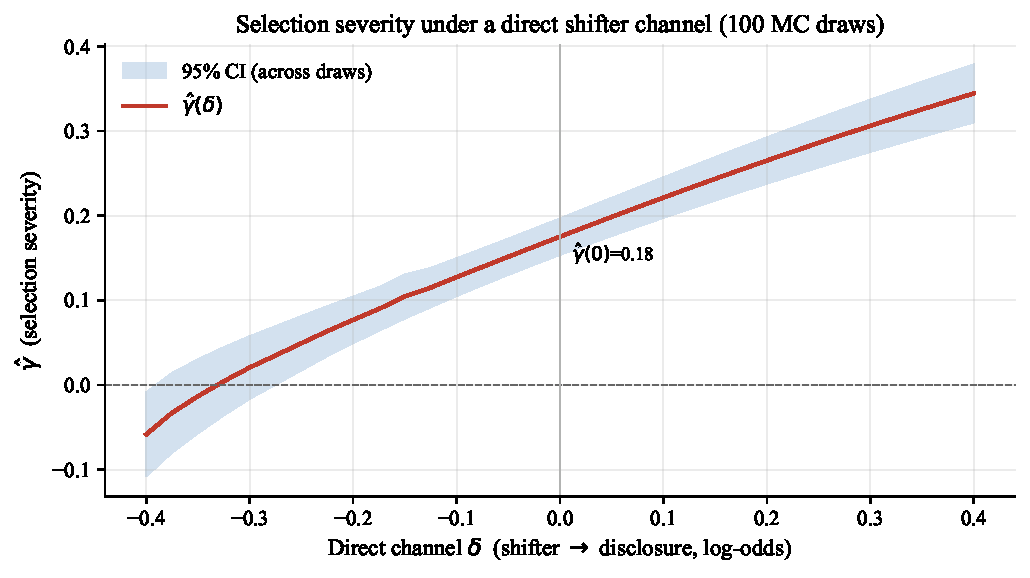
\includegraphics[width=0.72\linewidth]{figs/chr_sensitivity_inmc_baseline_wti_gind.pdf}
\caption{\textbf{Selection severity under a direct shifter channel.} Estimated
$\hat\gamma$ as a function of an imposed direct effect $\delta$ of the shifter on the
disclosure propensity, a violation of the exclusion restriction \eqref{eq:exclusion},
averaged across Monte Carlo draws with a band of $\pm1.96$ across-draw standard
errors. At $\delta=0$ the exclusion restriction holds and $\hat\gamma$ equals the
headline estimate. $\hat\gamma$ rises with $\delta$: the direct channel that
profitability or attention would induce (a positive $\delta$) strengthens selection,
and only a sizeable, wrong-signed negative $\delta$ -- the point estimate reaches
zero at $\delta \approx -0.34$, roughly six times the shifter's own reduced-form
association with disclosure -- drives $\hat\gamma$ to zero.}
\label{fig:chr_sensitivity}
\end{figure}

\subsection{Response mechanism}

We model the probability of emissions disclosure using a response mechanism that depends on firm characteristics and emissions, restating \eqref{eq:response_model} for convenience:
\begin{equation}
\label{eq:response_model_app}
\mathbb{P}(\delta_i = 1 \mid \mathbf{x}_{1i}, y_i)
=
\frac{\exp\{ f(\mathbf{x}_{1i}) + g(y_i) \}}
     {1 + \exp\{ f(\mathbf{x}_{1i}) + g(y_i) \}},
\end{equation}
where $\delta_i$ is the disclosure indicator, $\mathbf{x}_{1i}$ includes firm size and sector, and $g(y_i)$ captures the dependence of disclosure on emissions. 

We estimate the disclosure model~\eqref{eq:response_model} in two forms. In the fully parametric (FP) specification -- our primary specification -- $f(\mathbf{x}_{1,it})$ is linear in log assets and sector fixed effects and $g(y_{it}) = -\gamma y_{it}$ is linear in emissions, so the model is an ordinary logistic regression whose coefficient on $y_{it}$ estimates $-\hat\gamma$; this is the form the disclosure game implies (Lemma~\ref{lemma:indiv_best_resp}). In the semiparametric (SP) specification, $f$ and $g$ are generalized additive models with penalized splines on log assets and log emissions, allowing the disclosure response to vary nonlinearly \citep{yang2017semiparametric}. Comparing the two isolates the role of the linearity assumption; both are reported in Section~\ref{sec:measurement} and Appendix~\ref{app:robustness}.

\subsection{Exponential-tilt adjustment}

Given the estimated response mechanism, we correct the baseline imputations for selection using the exponential tilt of Corollary~\ref{cor:expo_tilt}. Under the logistic specification, the density of unobserved emissions differs from the observed density by a factor proportional to $\exp\{-g(y)\}$, which in the fully parametric case is $\exp\{\hat\gamma\, y\}$. We therefore reweight each imputation by $w_{it} \propto \exp\{\hat\gamma\, \hat{y}_{it}\}$ (equation~\eqref{eq:tilting_weights}), so that firms with lower disclosure probabilities -- the higher emitters -- receive greater weight, restoring the upper-tail mass that selection removes. Weights are trimmed at the 1st and 99th percentiles to limit the influence of extreme draws.

Intuitively, firms with emissions levels associated with a lower probability of disclosure receive greater weight in the adjusted distribution. This procedure restores right-tail mass that is systematically under-represented among reporting firms and yields selection-corrected estimates of firm-level and aggregate emissions.

\subsection{Monte Carlo sensitivity}

We quantify imputation uncertainty by repeating the imputation--tilt procedure across Monte Carlo draws. For each draw $b = 1, \dots, B$: (i) sample baseline imputations $\{\hat{y}_{it}^{(b)}\}$ for the non-disclosers from~\eqref{eq:baseline_imputation}; (ii) re-estimate the response mechanism~\eqref{eq:response_model} on the completed data; and (iii) form the tilting weights~\eqref{eq:tilting_weights} and compute the selection-corrected quantities. We report the mean and standard error across $B \in \{300, 500\}$ draws \citep{gohil2020multiple}. Because the missing-not-at-random restriction is not testable, these draws characterize sampling and specification variability rather than provide a formal test \citep{little2019statistical}.

\subsection{Robustness}
\label{app:robustness}
We probe the primary specification along four dimensions: the aggregate shock entering the excluded shifter, the granularity of the fixed effects, the functional form of the disclosure model, and the number of Monte Carlo draws. Each varies one element and holds the rest fixed. We also report the two identification diagnostics that motivate sample and reporting choices made in the body: the degeneracy of the disclosure margin off the major exchanges, and the sector-level disclosure rates behind the 10\% reporting threshold of Section~\ref{subsec:boundary}. Three of the four checks leave the correction essentially unchanged; the exception is fixed-effect granularity, where the tilt is sensitive in a direction we explain below and which makes our headline estimate the conservative one.

\paragraph{Where $\gamma$ is not identified.} Two of our design choices amount to the same rule -- do not report a selection severity where disclosure does not vary -- and we document the evidence for both here.

Table~\ref{tab:diag_exchange} rebuilds the panel without the exchange filter of Section~\ref{sec:data} and reports the disclosure margin by listing venue. The asymmetry is extreme. Among major-exchange firm-years, $11.7\%$ carry a disclosed Scope~1 figure. Among the $21{,}714$ off-exchange firm-years -- OTC, pink-sheet, and foreign venues -- \emph{seven} do: a disclosure rate of $0.03\%$. Estimating an emissions slope on that group anyway returns $|\hat\gamma| \approx 13$, an odds ratio of $e^{13}$ per standard deviation, which is not an economic magnitude but the numerical signature of a quasi-separated logit fit to seven positive outcomes.

\begin{table}[htbp]
\small
\centering
\caption{\textbf{Why the sample is restricted to major exchanges.} Panel~A reports the
disclosure margin by exchange group on the panel built \emph{without} the exchange filter.
\emph{Major} is NYSE, NYSE American, and Nasdaq (Compustat \texttt{exchg} 11, 12, 14);
\emph{Other} is all remaining listings (OTC, pink-sheet, and foreign venues). Panel~B
reports the emissions slope estimated separately by group, with sector, year, and
exchange-group fixed effects, emissions standardized within sector. The \emph{Other}
estimate is reported to show what the restriction removes: with 7 disclosers in
21,714 firm-years the logit is quasi-separated, so the coefficient is a numerical
artifact rather than a measure of disclosure behavior. The pooled row shows that these
firms do not in fact distort the pooled slope -- with so few disclosers they barely enter
the likelihood -- which is itself the argument for excluding them: they cannot inform
$\gamma$, yet retaining them would assign 19{,}097 firm-years a tilt extrapolated entirely
from firms whose disclosure margin they do not share. Panel~B is a diagnostic of
identification, not an estimate: it uses a single imputer draw and standardizes emissions
within sector, so its magnitudes are not comparable to Table~\ref{tab:results_LM}.}
\label{tab:diag_exchange}
\begin{tabular}{lrrrr}
\toprule
\multicolumn{5}{l}{\emph{Panel A: disclosure margin}} \\
\midrule
Exchange group & Firm-years & Firms & Disclosers & Disclosure rate \\
\midrule
Major & 59,388 & 7,944 & 6,920 & 11.652\% \\
Other & 21,714 & 3,629 & 7 & 0.032\% \\
\midrule
\multicolumn{5}{l}{\emph{Panel B: emissions slope, estimated by group}} \\
\midrule
Exchange group & \multicolumn{2}{r}{$\hat\gamma$} & \multicolumn{2}{r}{Std.\ error} \\
\midrule
Major & \multicolumn{2}{r}{+0.018} & \multicolumn{2}{r}{0.014} \\
Other & \multicolumn{2}{r}{+13.008} & \multicolumn{2}{r}{3.919} \\
Pooled & \multicolumn{2}{r}{+0.019} & \multicolumn{2}{r}{0.013} \\
\bottomrule
\end{tabular}
\end{table}


What this establishes is narrower than the natural argument suggests. These firms do \emph{not} distort the pooled estimate: the pooled slope ($+0.019$) is indistinguishable from the major-exchange slope ($+0.018$), because a group with seven disclosers contributes almost nothing to the likelihood of the emissions coefficient. The case for excluding them is the converse, and it is stronger. They cannot inform $\gamma$ at all, yet retaining them would assign $19{,}097$ firm-years an imputed emissions level and an exponential tilt whose selection severity \emph{and} outcome model are extrapolated wholesale from firms with whom they share no disclosure behavior. We would be recovering emissions for a population about whose disclosure decision the data are silent, and reporting the result as though it were measured. The restriction is therefore a statement about the reach of the estimator, not a claim that the excluded firms contaminate it.

The same pathology appears by sector, where Financials and Real Estate -- which disclose rarely and, per Appendix~\ref{app:methods}, lack the physical-capital exposure the instrument requires -- produce estimates an order of magnitude larger than any identified sector, with intervals to match. The next paragraph reports the sectoral cut and the threshold that removes them.

\paragraph{Sectoral heterogeneity in $\hat\gamma$.} Section~\ref{subsec:boundary} tests the audience boundary condition using within-sector institutional ownership, on the grounds that ownership is where the audience actually varies. It is natural to ask whether $\hat\gamma$ also differs across sectors, and Figure~\ref{fig:gamma_by_sector} reports that cut. We read it as descriptive rather than as a second test, for three reasons.

\begin{figure}[htbp]
    \centering
    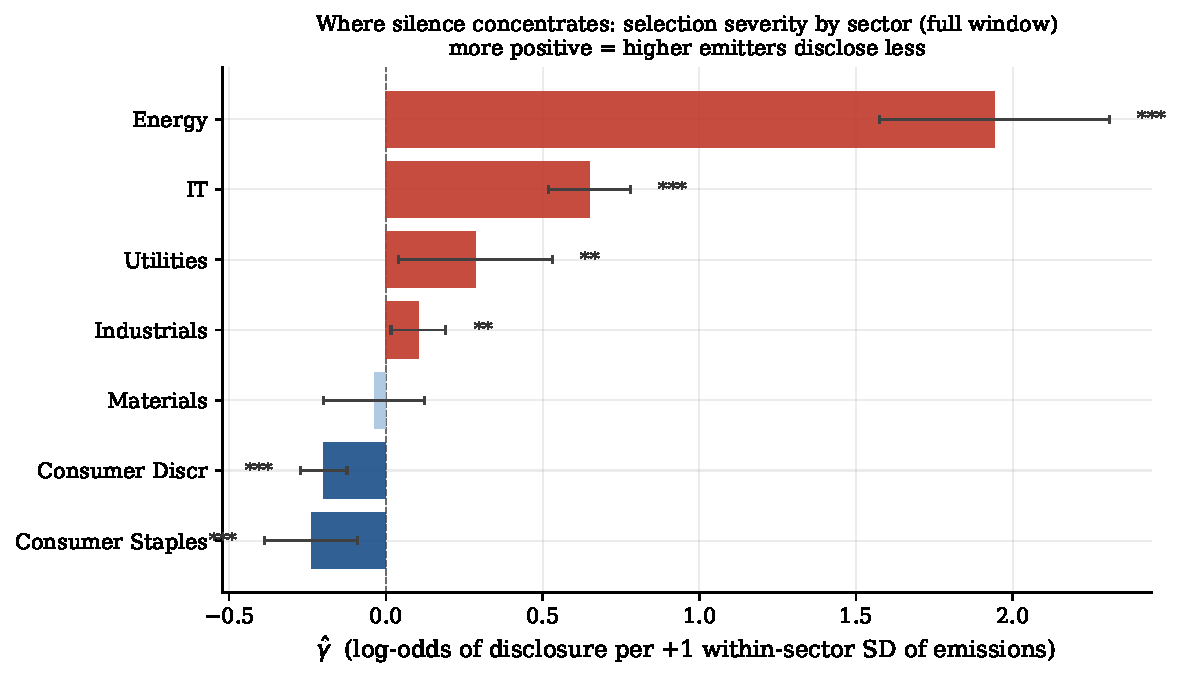
\includegraphics[width=0.95\linewidth]{figs/gamma_by_sector_fullwindow_tilt_test.pdf}
    \caption{\textbf{Selection severity by sector.} Estimated $\hat\gamma$ from a disclosure propensity model in which the emissions slope is interacted with GICS-11 sector, with 95\% confidence intervals. Emissions are standardized within sector, so $\hat\gamma$ is in log-odds per within-sector standard deviation and is comparable across sectors whose emission scales differ by orders of magnitude. Positive $\hat\gamma$ indicates strategic silence: higher emitters are less likely to disclose. The specification includes sector and year fixed effects and allows the size slope to differ by sector. Only sectors with a disclosure rate above 10\% are shown; below that threshold the logit is quasi-separated and $\hat\gamma$ is not identified. Stars denote significance at the 10\%, 5\%, and 1\% levels.}
    \label{fig:gamma_by_sector}
\end{figure}

First, $\gamma$ is identified only where disclosure varies, so we report $\hat\gamma$ only for sectors whose disclosure rate exceeds 10\%. This excludes Financials (6.5\%), Communication Services (7.4\%), Health Care (5.6\%), and Real Estate (3.3\%), whose unrestricted estimates run as high as $+38$ with intervals to match -- the numerical signature of quasi-separation, not evidence of extreme selection. The rule is specified in advance of inspecting the estimates and is the same one Section~\ref{sec:data} applies to off-exchange firms. It is worth recording that the threshold binds differently across samples: on the unfiltered all-exchange panel, where adding never-disclosing off-exchange firms dilutes every sector's rate, Information Technology falls from 11.1\% to 8.7\% and would drop out. A sectoral figure estimated on that panel would therefore look tidier than this one purely because a filter had removed an inconvenient sector, which is a reason to fix the sample first and read the figure second.

Second, the sectoral estimates are fragile to a restriction the ownership cut is robust to. Estimated freely, the size slope varies by a factor of roughly 64 across sectors, from $2.0\times10^{-5}$ in Consumer Discretionary to $1.3\times10^{-3}$ in Real Estate. Because size drives disclosure and is strongly correlated with emissions, constraining it to a common value pushes the misfit into the sector emissions slopes: doing so reverses the sign of $\hat\gamma$ for Industrials and Consumer Staples. We free the slope here and in Section~\ref{subsec:boundary}, where the same restriction spans only a factor of $1.25$ and changes nothing.

Third, and most fundamentally, sector bundles the audience with everything else that travels with an industry, and these need not point the same way. The EPA's Greenhouse Gas Reporting Program is the clearest case: it obliges facilities across 41 source categories to report once they emit 25{,}000 metric tons of CO$_2$ equivalent per year or more.\footnote{See \url{https://www.epa.gov/ghgreporting}. Reporting is to the regulator and does not itself constitute the voluntary public disclosure we measure, which is why the two come apart.} Regulatory attention of this kind raises the per-unit cost of revelation $c_1$ and pushes $\gamma$ up; but a firm already measuring and filing above the threshold faces a much lower marginal cost of also disclosing publicly, which lowers the cost of revelation for exactly the largest emitters and pushes $\gamma$ down. A sectoral $\hat\gamma$ is the net of forces this design cannot separate.

The pattern is accordingly mixed. Energy shows selection an order of magnitude stronger than any other sector ($+1.941^{***}$), which is what the mechanism implies for the environment where carbon is most salient to regulators and investors alike. The middle does not order itself so obligingly: Information Technology ($+0.650^{***}$) is second despite facing little carbon-specific Scope~1 scrutiny, while Consumer Staples ($-0.239^{***}$) and Consumer Discretionary ($-0.198^{***}$) show significant reverse selection; Utilities ($+0.285^{**}$), Industrials ($+0.104^{**}$), and Materials ($-0.037$, insignificant) fall between. Nor is the pattern a reflection of ownership composition: sector $\hat\gamma$ is uncorrelated with sector mean institutional ownership (Spearman $\rho = -0.36$, $p = 0.43$), which is unsurprising given that ownership ranges only from $0.56$ to $0.70$ across sectors. The middle sectors have no clean account, and we do not manufacture one.

\paragraph{Brownness proxy and standardisation.} The triple-difference test of Section~\ref{subsec:boundary} requires two choices: how to measure what a firm has to hide, and the scale in which $\hat\gamma$ is expressed. Table~\ref{tab:gamma_brown_robustness} reports all four combinations. The result is robust to the first choice and, for the primary proxy, to the second: with brownness measured by industry carbon intensity the triple difference is $+0.372$ under within-cell standardisation and $+0.389$ under within-sector standardisation, both significant at the $1\%$ level. Firm PP\&E intensity, which splits firms within industry rather than across, gives $+0.285$ under within-cell standardisation but only $+0.115$ ($p=0.23$) under within-sector standardisation. The divergence is a leverage artifact of the kind discussed in the main text: the four cells differ in how dispersed emissions are within them, so a slope denominated in sector-wide standard deviations is read outside the range some cells cover. That industry carbon intensity is insensitive to the convention while PP\&E intensity is not is why the former is the primary measure.

\begin{table}[htbp]
\footnotesize\centering
\caption{\textbf{The ownership gradient by brownness: proxy and standardisation robustness.}
Estimated $\hat\gamma$ in each cell of a within-sector institutional-ownership split crossed with a
brownness split, and the contrasts built from them. Columns~(1)--(2) define brownness by the carbon
intensity of a firm's GICS industry, computed from disclosing firms only; columns~(3)--(4) use the
firm's own PP\&E intensity. Within-cell standardisation expresses $\hat\gamma$ per standard deviation
of emissions present in that cell; within-sector standardisation uses the sector-wide standard
deviation throughout. All specifications include sector, year and ownership fixed effects and free
the size slope across cells.}
\label{tab:gamma_brown_robustness}
\begin{tabular}{lcccc}
\toprule
 & \multicolumn{2}{c}{Industry carbon intensity} & \multicolumn{2}{c}{Firm PP\&E intensity} \\
\cmidrule(lr){2-3}\cmidrule(lr){4-5}
 & (1) & (2) & (3) & (4) \\
 & within cell & within sector & within cell & within sector \\
\midrule
\multicolumn{5}{l}{\emph{Panel A: $\hat\gamma$ by ownership-by-brownness cell}} \\[2pt]
Low IO, clean & +0.071 & +0.275$^{***}$ & +0.135$^{***}$ & +0.034 \\
 & (0.048) & (0.101) & (0.048) & (0.063) \\
Low IO, brown & -0.140$^{***}$ & -0.196$^{***}$ & -0.042 & -0.145$^{***}$ \\
 & (0.034) & (0.031) & (0.032) & (0.030) \\
High IO, clean & -0.076$^{***}$ & +0.212$^{***}$ & +0.088$^{***}$ & +0.226$^{***}$ \\
 & (0.026) & (0.059) & (0.028) & (0.066) \\
High IO, brown & +0.085$^{***}$ & +0.130$^{***}$ & +0.196$^{***}$ & +0.163$^{***}$ \\
 & (0.031) & (0.023) & (0.033) & (0.022) \\
\midrule
\multicolumn{5}{l}{\emph{Panel B: contrasts}} \\[2pt]
Ownership gap, brown & +0.225$^{***}$ & +0.327$^{***}$ & +0.238$^{***}$ & +0.308$^{***}$ \\
 & (0.045) & (0.039) & (0.046) & (0.037) \\
Ownership gap, clean & -0.147$^{***}$ & -0.063 & -0.047 & +0.192$^{**}$ \\
 & (0.054) & (0.114) & (0.056) & (0.090) \\
Triple difference & +0.372$^{***}$ & +0.389$^{***}$ & +0.285$^{***}$ & +0.115 \\
 & (0.070) & (0.119) & (0.071) & (0.096) \\
\midrule
Observations & 40,792 & 40,792 & 41,287 & 41,287 \\
\bottomrule
\end{tabular}
\begin{flushleft}\footnotesize
\textit{Notes:} The triple difference is the ownership gap among brown firms minus the ownership
gap among clean firms, with a delta-method standard error from the full coefficient covariance.
Industry carbon intensity is robust to the standardisation convention; PP\&E intensity is not,
which is why the former is the primary measure in Section~\ref{subsec:boundary}.
Significance: $^{***}p<0.01$, $^{**}p<0.05$, $^{*}p<0.10$.
\end{flushleft}
\end{table}

\paragraph{Alternative shifters.} The shift-share instrument combines an aggregate shock with a predetermined firm-level exposure. We vary the shock, replacing $\log(\mathrm{WTI}_t)$ with log U.S.\ real GDP while holding the exposure and every other element of the specification fixed, so that the shock is the only thing that changes (Table~\ref{tab:OutcomeModel_baseline_gdp_gsec}). The substitution leaves the results essentially untouched: the shifter remains strongly relevant in the outcome model ($\hat\eta_2 = 0.348$, s.e.\ $0.011$, against $0.188$ under WTI), the fit is identical to three decimals ($R^2 = 0.809$ under both, on the same 6{,}698 disclosers), the size elasticity is unchanged ($0.970$ versus $0.968$), and the tilt correction moves from $+11.9\%$ to $+11.5\%$.

This near-equivalence is a structural feature of the estimator rather than a coincidence, and it is worth stating explicitly because two nearly identical columns invite the suspicion that the instrument does no work. The selection severity is identified from the propensity model, which \emph{excludes} the shifter by construction; the shifter enters only through the outcome model, where it shapes the imputed emissions of non-disclosers. Two shocks that shift emissions comparably therefore deliver comparable $\hat\gamma$, and the correct reading of the stability is the reassuring one: $\hat\gamma$ is not an artifact of which aggregate series we interact with exposure. What the exercise does \emph{not} test is the exposure side of the shift-share, which is where the identifying within-year variation actually comes from; we take that up next.


\paragraph{Fixed-effect granularity.} The baseline uses GICS industry fixed effects. Re-estimating with the coarser GICS-11 sector classification, holding the WTI shifter and the sample fixed (Table~\ref{tab:OutcomeModel_baseline_wti_gsec}), leaves the qualitative structure intact: the size elasticity remains near one ($1.027$ versus $0.968$), the shifter remains strongly relevant ($\hat\eta_2 = 0.271$), and the brown/green ordering is preserved, with Utilities ($+3.79$), Materials ($+3.48$), and Energy ($+3.14$) at the top and Financials ($-1.70$) at the bottom. The fit falls as expected with fewer effects ($R^2 = 0.738$ versus $0.809$).

The correction, however, is \emph{not} invariant to this choice, and we report the sensitivity rather than smooth it over. Under sector fixed effects the tilt rises to $+21.6\%$, against $+11.9\%$ under industry effects -- close to double. The mechanism is transparent and, in our reading, favors the baseline. Coarser fixed effects leave more genuine cross-firm heterogeneity in emissions unexplained, inflating the residual variance $\sigma^2$ of the outcome model; since the Gaussian bias in \eqref{eq:gaussian_bias} scales as $\Delta\mu = \gamma\sigma_1^2$, a fatter residual distribution mechanically produces a larger tilt for the same selection severity. The sector specification is thus attributing to selection what is in fact unmodeled industry technology. This is precisely why we adopt the finer industry fixed effects as the baseline: they absorb the production-side variation that the tilt would otherwise misread as strategic silence, and they make the reported correction the \emph{conservative} of the two. A reader who prefers the coarser specification should read our headline figure as a lower bound.

\begin{table}[htbp]
\footnotesize
\centering
\caption{\textbf{Outcome model, coarser fixed effects (robustness).} Linear regression of log Scope~1 emissions on firm characteristics, the shift-share oil shifter, GICS-11 \emph{sector} indicators, and year fixed effects. Identical to the baseline of Table~\ref{tab:OutcomeModel_baseline_wti_gind} except that the finer GICS industry effects are replaced by sector effects; sample, shifter, and all other choices are held fixed. Robust standard errors in parentheses. Significance levels: $^{***}p<0.01$, $^{**}p<0.05$, $^{*}p<0.1$.}
\label{tab:OutcomeModel_baseline_wti_gsec}
\begin{tabular}{l c}
\toprule
 & Log Scope~1 Emissions \\
\midrule
\textit{Macroeconomic and firm characteristics} \\
$z_{it}$ (oil-price shifter) & 0.2706$^{***}$ \\
      & (0.006) \\
$\log(\mathrm{Assets}_i)$ & 1.0271$^{***}$ \\
      & (0.014) \\
Constant & 0.2258 \\
      & (0.206) \\

\midrule
\textit{Sector fixed effects (baseline: Communication Services)} \\
Consumer Discr & 1.3687$^{***}$ \\
Consumer Staples & 2.7184$^{***}$ \\
Energy & 3.1446$^{***}$ \\
Financials & -1.6971$^{***}$ \\
Health Care & 1.0760$^{***}$ \\
IT & 0.5986$^{***}$ \\
Industrials & 2.3802$^{***}$ \\
Materials & 3.4809$^{***}$ \\
Real Estate & 1.2097$^{***}$ \\
Utilities & 3.7898$^{***}$ \\

\midrule
\textit{Year fixed effects (baseline: 2012)} \\
2013 & -0.0397 \\
2014 & -0.0832 \\
2015 & -0.0705 \\
2016 & -0.1043 \\
2017 & -0.2100$^{*}$ \\
2018 & -0.2606$^{**}$ \\
2019 & -0.3124$^{***}$ \\
2020 & -0.3439$^{***}$ \\
2021 & -0.5152$^{***}$ \\
2022 & -0.5612$^{***}$ \\
2023 & -0.7031$^{***}$ \\

\midrule
Observations & 6,698 \\
$R^2$ & 0.738 \\
\bottomrule
\end{tabular}

\begin{flushleft}
\footnotesize
\end{flushleft}
\end{table}

\begin{table}[htbp]
\footnotesize
\centering
\caption{\textbf{Outcome model, alternative shock (robustness).} Linear regression of log Scope~1 emissions on firm characteristics, the shift-share shifter built from log U.S.\ real GDP in place of the WTI crude price, GICS industry indicators, and year fixed effects. Identical to the baseline of Table~\ref{tab:OutcomeModel_baseline_wti_gind} except for the aggregate shock; the predetermined firm exposure, the sample, and all other choices are held fixed. Robust standard errors in parentheses. Significance levels: $^{***}p<0.01$, $^{**}p<0.05$, $^{*}p<0.1$.}
\label{tab:OutcomeModel_baseline_gdp_gsec}
\begin{tabular}{l c}
\toprule
 & Log Scope~1 Emissions \\
\midrule
\textit{Macroeconomic and firm characteristics} \\
$z_{it}$ (GDP shifter) & 0.3476$^{***}$ \\
      & (0.011) \\
$\log(\mathrm{Assets}_i)$ & 0.9697$^{***}$ \\
      & (0.013) \\
Constant & 3.8844$^{***}$ \\
      & (0.183) \\

\midrule
\textit{Year fixed effects (baseline: 2012)} \\
2013 & -0.0802 \\
2014 & -0.1244 \\
2015 & -0.1620 \\
2016 & -0.2277$^{**}$ \\
2017 & -0.3136$^{***}$ \\
2018 & -0.3287$^{***}$ \\
2019 & -0.3791$^{***}$ \\
2020 & -0.4537$^{***}$ \\
2021 & -0.5541$^{***}$ \\
2022 & -0.5822$^{***}$ \\
2023 & -0.7101$^{***}$ \\

\midrule
\midrule
\textit{Industry fixed effects (baseline: Energy Equipment \& Services)} & YES \\
Observations & 6,698 \\
$R^2$ & 0.809 \\
\bottomrule
\end{tabular}

\begin{flushleft}
\footnotesize
\end{flushleft}
\end{table}

\paragraph{Functional form.} We compare the fully parametric (FP) disclosure model with a semiparametric generalized additive model (SP) -- specifically, a Logistic Generalized Additive Model (LogisticGAM). This approach introduces multiple spline regressors, allowing for greater flexibility in capturing non-linear relationships between the covariates and the probability of disclosure, and without requiring any specification of the response model. However, this increased flexibility comes at the cost of interpretability, as the estimated coefficients vary across the range of the covariates. 

\begin{figure}[htbp]
\centering
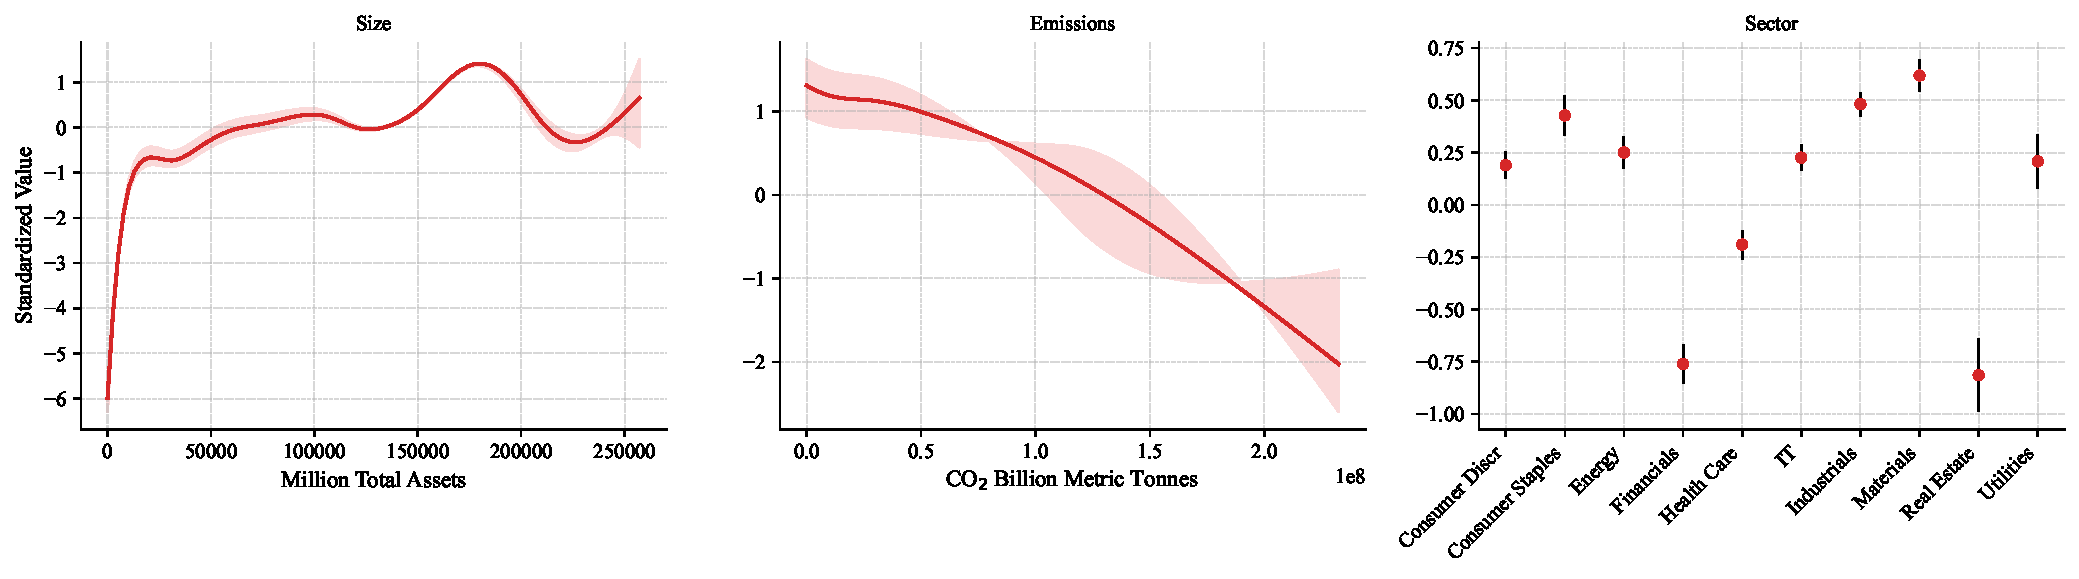
\includegraphics[width=0.95\linewidth]{figs/response_box_plot_gam_baseline_wti_gind.pdf}
\caption{\textbf{Semiparametric response mechanism.} Distribution of standardized coefficients from the GAM disclosure model across $B=300$ Monte Carlo draws: firm size (left), Scope~1 emissions (centre), and sector indicators (right). Red lines mark the mean across draws; bands and whiskers show variability across draws. The emissions--disclosure relationship is approximately linear and negative, supporting the linear specification the disclosure game implies.}
\label{fig:response_gam}
\end{figure}

Figure \ref{fig:response_gam} presents the estimated standardized coefficient values for firm size, Scope 1 emissions, and the sector covariates, on the probability of emissions disclosure, along with their respective 95\% confidence intervals. The left panel illustrates a non-linear relationship between firm size and disclosure. Specifically, the effect increases rapidly for small- to mid-sized firms and then stabilizes, indicating diminishing marginal effects at higher asset levels.  Interestingly, firms in the lowest asset quantile exhibit a negative coefficient, suggesting that very small companies are less likely to disclose, potentially due to the fixed costs of reporting and limited regulatory and stakeholder pressure. 

The middle panel highlights a clear, approximately linear negative relationship between Scope 1 emissions and disclosure likelihood. As emissions increase, the associated coefficient steadily declines, implying that firms with higher emissions are systematically less likely to disclose. This pattern is consistent with non-random disclosure, in which higher emitters are less likely to disclose, aligning with the MNAR framework adopted in the analysis.

The right panel displays the estimated sectoral effects relative to the baseline (Communication Services). Results align with fully parametric ones. Most sectors exhibit positive coefficients, indicating a higher probability of disclosure compared to the baseline. 

Despite the advantages of the semi-parametric approach in capturing complex relationships, its interpretability remains limited due to the non-parametric nature of the splines. Nonetheless, the trends observed align with expectations and provide a nuanced understanding of the covariates' influence on disclosure probability, while validating the robustness of the fully parametric results. The tilt correction is larger under the SP model (about $+19.1\%$ versus $+12.4\%$ under FP at $B=500$; $+19.4\%$ versus $+11.9\%$ at $B=300$; Table~\ref{tab:emissions_tilts}), reflecting the additional upper-tail flexibility of the splines. We adopt FP as primary because it is the specification the disclosure game implies, and read the SP figure as an upper bound on the correction: the two bracket the plausible range, and the qualitative conclusion -- that MAR imputation understates emissions materially, and understates them in the tail -- holds under either. The gap between them is itself informative. It says the linear $g(y)$ is mildly conservative relative to a flexible fit, which is the direction of error we would rather make, since the tilt compounds any overstatement of $\hat\gamma$ into the aggregate.

\paragraph{Monte Carlo draws.} All Monte Carlo quantities are reported for both $B = 300$ and $B = 500$ draws (Tables~\ref{tab:results_LM} and~\ref{tab:emissions_tilts}). The means are essentially identical across the two, indicating that the procedure has converged and that $300$ draws suffice.

\paragraph{Alternative vendor and market.} The correction should be a property of the selection model, not of one vendor's emissions estimates or one market. To check this we re-run the entire measurement pipeline -- outcome model, disclosure propensity, and exponential tilt -- on two samples constructed independently of the Trucost data used in the body: U.S.\ firms with emissions from Refinitiv in place of Trucost, and European firms from Refinitiv. Table~\ref{tab:vendor_market_robustness} reports the pooled selection severity and the implied tilt for all three, alongside the outcome-model diagnostics that establish the first stage behaves the same way throughout. The severity is positive, significant, and of comparable magnitude everywhere -- $\hat\gamma$ between $0.15$ and $0.24$ -- so that higher emitters disclose less is neither an artifact of Trucost's estimation procedure nor specific to the United States. The correction it implies moves with it: the tilt is largest where $\hat\gamma$ is largest (Refinitiv U.S., $+16.8\%$) and smallest where it is smallest (Europe, $+6.1\%$), with Trucost between, the ordering a mechanical scaling of the tilt by the severity predicts and a stronger signal than any single point estimate. The smaller European figure is itself interpretable rather than noise: European firms disclose at higher rates and under a tightening mandatory regime, so less emissions mass is hidden for the tilt to recover.\footnote{This exercise validates the measurement -- the detection of selection and the magnitude of the correction -- across vendor and market. It bears on the imputation of Section~\ref{sec:measurement}, not on the pricing results of Section~\ref{sec:pricing}, which use U.S.\ Trucost emissions and CRSP returns throughout.}

The outcome-model columns confirm that these are not comparable $\hat\gamma$'s extracted from broken first stages. The size elasticity is essentially one in all three samples ($0.97$ to $1.03$), so emissions scale with firm size identically regardless of vendor or market; the fit is comparable ($R^2$ of $0.72$ to $0.81$); and each is estimated on several thousand disclosers. The excluded shifter is relevant everywhere, though not equally so: its coefficient is around $0.19$--$0.20$ in the two U.S.\ samples but $0.077$ in Europe. The European instrument is weaker because Europe's energy mix is less oil-intensive, so an oil-price shift-share moves European emissions less; it remains significant at the $1\%$ level, so identification holds, but the reduced identifying variation is one reason to read the European estimates as corroborating rather than co-equal.

\begin{table}[htbp]
\footnotesize\centering
\caption{\textbf{The MNAR correction across vendor and market.} Pooled selection
severity $\hat\gamma$ and the tilt uplift of average imputed Scope~1 emissions over
the missing-at-random baseline, with the outcome-model diagnostics, from re-running
the full pipeline on three independently constructed samples. Emissions are from
Trucost in the body row and from Refinitiv in the two robustness rows.}
\label{tab:vendor_market_robustness}
\begin{tabular}{ll cc ccc}
\toprule
 & & \multicolumn{2}{c}{Correction} & \multicolumn{3}{c}{Outcome model} \\
\cmidrule(lr){3-4}\cmidrule(lr){5-7}
Market & Vendor & $\hat\gamma$ & Tilt & $\hat\eta_2$ & $R^2$ & $N$ \\
\midrule
United States & Trucost (body) & $0.18^{***}$ & $+12.4\%$ & $0.188^{***}$ & $0.81$ & $6{,}698$ \\
United States & Refinitiv      & $0.24^{***}$ & $+16.8\%$ & $0.200^{***}$ & $0.72$ & $9{,}097$ \\
Europe        & Refinitiv      & $0.15^{***}$ & $+6.1\%$  & $0.077^{***}$ & $0.73$ & $13{,}230$ \\
\bottomrule
\end{tabular}
\begin{flushleft}\footnotesize
\textit{Notes:} $\hat\gamma$ is the standardized emissions slope of the disclosure
propensity, in the model convention ($\hat\gamma>0$ denotes higher emitters
disclosing less); its significance is read from the year-by-year estimates, which
are significant at the $1\%$ level in every U.S.\ year and in the strong early and
late European years, so the pooled estimate is significant a fortiori. The tilt is
$(\bar{y}^{\text{adj}} - \bar{y}^{\text{base}})/\bar{y}^{\text{base}}$ from the Monte
Carlo run. $\hat\eta_2$ is the coefficient on the excluded oil-price shifter in the
outcome model, and $R^2$ and $N$ (disclosing firm-years) are outcome-model
quantities; the size elasticity, not tabulated, is $0.97$, $1.00$, and $1.03$
respectively. Significance: $^{***}p<0.01$, $^{**}p<0.05$, $^{*}p<0.10$.
\end{flushleft}
\end{table}

\clearpage

\section{Tables}
\label{app:data}

\subsection{Sample Statistics}

\begin{table}[htbp]
\centering
\small
\caption{\textbf{Sample construction.} Firm-year observations retained at each step, from the raw Compustat North America fundamentals extract to the estimation sample. The exchange restriction and the predetermined-exposure requirement are discussed in the text.}
\label{tab:sample_funnel}
\begin{tabular}{l r r}
\toprule
Step & Firm-years & Dropped \\
\midrule
Compustat North America fundamentals                          & 161{,}717 & \\
\quad Non-missing identifiers and core financials             & 145{,}805 & 15{,}912 \\
\quad Major U.S.\ exchanges (NYSE, NYSE American, Nasdaq)     &  89{,}637 & 56{,}168 \\
\quad Merged to Trucost Environmental and macro series        &  71{,}261 & 18{,}376 \\
\quad Valid disclosure classification and total assets        &  69{,}746 &  1{,}515 \\
\quad Sample window 2012--2023                                &  59{,}996 &  9{,}750 \\
\quad Total assets trimmed at 1st/99th percentile within year &  58{,}796 &  1{,}200 \\
\quad Predetermined PP\&E exposure available                  &  51{,}355 &  7{,}441 \\
\midrule
\textbf{Estimation sample}                                    & \textbf{51{,}355} & \\
\quad \emph{Unique firms}                                     & 6{,}938 & \\
\quad \emph{Average firms per year}                           & 4{,}280 & \\
\quad \emph{Share with disclosed Scope~1}                     & 13.0\% & \\
\bottomrule
\end{tabular}
\end{table}

\begin{center}
\begin{table}[htbp]
\small
\caption{\textbf{Sample Summary Statistics}. Data are extracted from Trucost Environmental and Compustat, for US public companies from 2012 to 2023. Data are yearly values. Total Market Value is in trillion USD. Total CO$_2$ Emissions are Scope 1 Emissions, measured in billions of metric tons (Gt), both disclosed by companies and estimated by Trucost. Average CO$_2$ intensity is computed as total emissions per total assets of each company, in Tons of CO$_2$ over Millions USD.}\label{table:summary_stats}
\begin{center}
\begin{tabular}{p{0.8cm} c >{\centering\arraybackslash}p{3.5cm} >{\centering\arraybackslash}p{4cm} >{\centering\arraybackslash}p{1.8cm}}
\hline
Year & N & Total Mkt Value & Scope 1 Emissions & Intensity\footnotemark\\
\hline 
\hline
2012 & 4739 & 15.21 & 2.18 & 287.81 \\
2013 & 4821 & 19.13 & 2.22 & 279.53 \\
2014 & 4786 & 21.22 & 2.23 & 266.77 \\
2015 & 4739 & 19.99 & 2.10 & 261.67 \\
2016 & 4716 & 21.18 & 2.20 & 166.12 \\
2017 & 4717 & 25.22 & 2.35 & 164.06 \\
2018 & 4727 & 23.30 & 2.45 & 157.98 \\
2019 & 4862 & 26.32 & 2.33 & 164.13 \\
2020 & 5014 & 30.47 & 2.13 & 162.95 \\
2021 & 5149 & 38.16 & 2.32 & 150.84 \\
2022 & 5232 & 30.13 & 2.19 & 109.79 \\
2023 & 5294 & 35.70 & 2.06 & 104.63 \\[0.2em]
\hline
\end{tabular}
\label{tab:summaryStats}  
\end{center}
\end{table}
\end{center} 



\footnotetext{CO$_2$ Emission divided by total assets of a company (CO$_2$ Metric Tonnes per \$Million).}

\begin{table}[htbp]
\small
\centering
\caption{\textbf{Summary statistics by year and disclosure status.} Firms are split by whether Scope~1 emissions are directly disclosed (\emph{Observed}) or are absent or vendor-estimated (\emph{Missing}); see Table~\ref{tab:disclosure_groups} for the classification. Total market value is in trillion USD; Scope~1 emissions in billions of metric tons (Gt); intensity is emissions per total assets (tCO$_2$ per \$Million). Figures describe the sample after the asset trim and before the predetermined-exposure requirement (58{,}796 firm-years; see Table~\ref{tab:sample_funnel}).}
\label{tab:summary_disclosure}
\begin{tabular}{l rr rr rr rr}
\toprule
& \multicolumn{2}{c}{$N$} & \multicolumn{2}{c}{Total Mkt Value} & \multicolumn{2}{c}{Scope~1 Emissions} & \multicolumn{2}{c}{Intensity} \\
\cmidrule(lr){2-3} \cmidrule(lr){4-5} \cmidrule(lr){6-7} \cmidrule(lr){8-9}
Year & Missing & Obs. & Missing & Obs. & Missing & Obs. & Missing & Obs. \\
\midrule
2012 & 4{,}434 &   305 &  7.27 &  7.95 & 0.39 & 1.79 & 151.85 & 464.34 \\
2013 & 4{,}501 &   320 &  9.21 &  9.92 & 0.27 & 1.95 & 148.96 & 470.90 \\
2014 & 4{,}452 &   334 &  9.98 & 11.25 & 0.20 & 2.03 & 125.16 & 464.78 \\
2015 & 4{,}402 &   337 &  9.48 & 10.50 & 0.31 & 1.79 & 142.25 & 433.18 \\
2016 & 4{,}335 &   381 &  9.37 & 11.81 & 0.41 & 1.80 & 107.47 & 420.27 \\
2017 & 4{,}294 &   423 & 11.06 & 14.16 & 0.42 & 1.93 & 106.25 & 400.22 \\
2018 & 4{,}243 &   484 &  9.14 & 14.15 & 0.46 & 1.99 &  97.08 & 378.45 \\
2019 & 4{,}298 &   564 & 10.00 & 16.31 & 0.25 & 2.09 &  82.75 & 414.34 \\
2020 & 4{,}287 &   727 & 11.49 & 18.98 & 0.19 & 1.94 &  68.02 & 413.66 \\
2021 & 4{,}231 &   918 & 10.44 & 27.73 & 0.21 & 2.11 &  58.48 & 336.16 \\
2022 & 4{,}107 & 1{,}125 &  6.34 & 23.79 & 0.11 & 2.07 &  43.11 & 224.00 \\
2023 & 4{,}320 &   974 &  9.51 & 26.19 & 0.25 & 1.81 &  51.08 & 219.44 \\
\bottomrule
\end{tabular}
\end{table}

\clearpage

\begin{landscape}
\begin{table}[h!]
\centering
\caption{\textbf{Sources of Scope 1 emissions data, 2023 snapshot}.}
\label{tab:emissions_sources}
\begin{tabular}{lccc}
\toprule
\textbf{Disclosure source} & \textbf{Count} & \textbf{Share (\%)} & \textbf{Treatment} \\
\midrule
\multicolumn{4}{l}{\textit{Vendor-estimated emissions}} \\
Estimated data & 1{,}894 & 35.78 & Missing \\
Derived from previous year & 173 & 3.27 & Missing \\
Value derived from fuel use provided in Environmental/CSR & 12 & 0.23 & Missing \\
Value derived from fuel use provided in Annual Report/Financial Accounts Disclosure & 6 & 0.11 & Missing \\
Estimate based on partial data disclosure in Environmental/CSR & 2 & 0.04 & Missing \\
Estimate based on partial data disclosure in Annual Report/10-K/Financial Accounts & 1 & 0.02 & Missing \\
\midrule
\multicolumn{4}{l}{\textit{Firm-reported emissions (CSR / Environmental reports)}} \\
Value derived from data provided in Environmental/CSR & 724 & 13.68 & Observed \\
Exact Value from Environmental/CSR & 104 & 1.96 & Observed \\
Value summed up from data provided in Environmental/CSR & 29 & 0.55 & Observed \\
Value split from data provided in Environmental/CSR & 9 & 0.17 & Observed \\
\midrule
\multicolumn{4}{l}{\textit{Firm-reported emissions (CDP)}} \\
Exact Value from CDP & 52 & 0.98 & Observed \\
Value derived from data provided in CDP & 30 & 0.57 & Observed \\
\midrule
\multicolumn{4}{l}{\textit{Firm-reported emissions (Annual reports / 10-Ks)}} \\
Value derived from data provided in Annual Report/Financial Accounts Disclosure & 22 & 0.42 & Observed \\
Exact Value from Annual Report/10K/Financial Accounts Disclosure & 2 & 0.04 & Observed \\
Value summed up from data provided in Annual Report/Financial Accounts Disclosure & 1 & 0.02 & Observed \\
Value split from data provided in Annual Report/Financial Accounts Disclosure & 1 & 0.02 & Observed \\
\midrule
\multicolumn{4}{l}{\textit{Missing}} \\
None & 2{,}232 & 42.16 & Missing \\
\midrule
\textbf{Total} & \textbf{5,294} & \textbf{100.00} & \\
\bottomrule
\end{tabular}
\end{table}
\end{landscape}


\clearpage

\subsection{Outcome Model Results}

\begin{table}[htbp]
\footnotesize
\centering
\caption{\textbf{Outcome model results.} Linear regression of log Scope~1 emissions on firm characteristics, macroeconomic conditions, industry indicators, and year fixed effects. Robust standard errors in parentheses. Significance levels: $^{***}p<0.01$, $^{**}p<0.05$, $^{*}p<0.1$.}
\label{tab:OutcomeModel_baseline_wti_gind}
\begin{tabular}{l c}
\toprule
 & Log Scope~1 Emissions \\
\midrule
\textit{Macroeconomic and firm characteristics} \\
Oil exposure $\times \log(\mathrm{WTI}_t)$  & 0.1883$^{***}$ \\
      & (0.006) \\
$\log(\mathrm{Assets}_i)$ & 0.9675$^{***}$ \\
      & (0.013) \\
Constant & 3.8807$^{***}$ \\
      & (0.183) \\

\midrule
\textit{Year fixed effects (baseline: 2012)} \\
2013 & -0.0851 \\
2014 & -0.1237 \\
2015 & -0.1097 \\
2016 & -0.1666 \\
2017 & -0.2634$^{***}$ \\
2018 & -0.2994$^{***}$ \\
2019 & -0.3385$^{***}$ \\
2020 & -0.3849$^{***}$ \\
2021 & -0.5284$^{***}$ \\
2022 & -0.5748$^{***}$ \\
2023 & -0.6915$^{***}$ \\

\midrule
\midrule
\textit{Industry fixed effects (baseline: Energy Equipment \& Services)} & YES\\
Observations & 6,698 \\
$R^2$ & 0.809 \\
\bottomrule
\end{tabular}



\begin{flushleft}
\footnotesize
\end{flushleft}
\end{table}

\clearpage

\subsection{Response Mechanism Results}

\begin{table}[htbp]
\footnotesize
\centering
\caption{\textbf{Response mechanism: fully parametric model.}
Mean coefficient estimates and standard errors from Monte Carlo simulations.
Results are reported for $B=300$ and $B=500$ draws.}
\label{tab:results_LM}

\begin{tabular}{lcccc}
\toprule
 & \multicolumn{2}{c}{$B=300$} & \multicolumn{2}{c}{$B=500$} \\
\cmidrule(lr){2-3} \cmidrule(lr){4-5}
 & Mean & SE & Mean & SE \\
\midrule
\textit{Firm characteristics} \\
Constant   & -2.9154 & 0.0112 & -2.9165 & 0.0118 \\
Size       &  1.8701 & 0.0265 &  1.8722 & 0.0275 \\
Emissions  & -0.1953 & 0.0727 & -0.1994 & 0.0743 \\
\midrule
\textit{Sector effects (baseline: Communication Services)} \\
Consumer Discretionary &  1.4806 & 0.0067 &  1.4812 & 0.0069 \\
Consumer Staples       &  2.0418 & 0.0063 &  2.0423 & 0.0065 \\
Energy                 &  1.4992 & 0.0171 &  1.5004 & 0.0177 \\
Financials             & -0.3936 & 0.0026 & -0.3938 & 0.0027 \\
Health Care            &  0.1659 & 0.0057 &  0.1663 & 0.0059 \\
IT                     &  1.3505 & 0.0076 &  1.3511 & 0.0078 \\
Industrials            &  1.8437 & 0.0108 &  1.8445 & 0.0111 \\
Materials              &  2.3713 & 0.0185 &  2.3725 & 0.0191 \\
Real Estate            & -0.0703 & 0.0066 & -0.0698 & 0.0068 \\
Utilities              &  1.9695 & 0.0728 &  1.9741 & 0.0751 \\
\midrule
\textit{Year fixed effects (baseline: 2012)} \\
2013 & 0.0903 & 0.0044 & 0.0907 & 0.0048 \\
2014 & 0.0619 & 0.0042 & 0.0618 & 0.0041 \\
2015 & 0.1035 & 0.0042 & 0.1034 & 0.0043 \\
2016 & 0.3242 & 0.0045 & 0.3242 & 0.0044 \\
2017 & 0.4613 & 0.0049 & 0.4611 & 0.0049 \\
2018 & 0.6256 & 0.0050 & 0.6255 & 0.0049 \\
2019 & 0.8757 & 0.0043 & 0.8757 & 0.0044 \\
2020 & 1.1888 & 0.0049 & 1.1888 & 0.0049 \\
2021 & 1.4502 & 0.0046 & 1.4502 & 0.0045 \\
2022 & 1.8248 & 0.0043 & 1.8248 & 0.0043 \\
2023 & 1.6377 & 0.0042 & 1.6377 & 0.0042 \\
\bottomrule
\end{tabular}

\begin{flushleft}
\footnotesize
\textit{Notes:} Coefficients are standardized. Results are based on repeated simulations of the response mechanism estimated on imputed emissions.
\end{flushleft}
\end{table}

\clearpage

\subsection{The tilting correction}


\begin{table}[htbp]
\small
\centering
\caption{Summary statistics (mean and standard deviation, in metric tonnes CO$_2$) of firm-level Scope~1 emissions under different imputation strategies: the missing-at-random baseline (non-tilted), and the MNAR correction under the fully parametric (FP) and semiparametric (SP) response models.}
\label{tab:emissions_tilts}
\begin{tabular}{lcccc}
\toprule
 & \multicolumn{2}{c}{$B=300$} & \multicolumn{2}{c}{$B=500$} \\
\cmidrule(lr){2-3} \cmidrule(lr){4-5}
 & Mean & St.\ Dev. & Mean & St.\ Dev. \\
\midrule
MAR        & 954,567  & 44,110  & 957,284 & 46,054  \\
MNAR (FP)  & 1,068,600 & 80,314 & 1,075,583  & 86,510 \\
MNAR (SP)  & 1,139,399 & 82,840 & 1,139,831 & 84,642 \\
\bottomrule
\end{tabular}
\end{table}

\clearpage

\subsection{Pricing Emissions Intensity}

\begin{table}[htbp]
\footnotesize\centering
\caption{\textbf{Emissions Intensity and Stock Returns: Firm-Reported versus Vendor.}
Panel regressions of monthly returns on standardized log Scope~1 emissions
\emph{intensity} (emissions over revenue), the specification of
\citet{aswani2024carbon}. Column~(1) uses firm-reported emissions only;
column~(2) adds vendor-estimated firms; column~(3) is the full Compustat
universe. Panel~A uses observed values, Panels~B and~C the MNAR-corrected and
MAR-imputed measures. Standard errors clustered at the firm level.}
\label{tab:returns_intensity}
\begin{tabular}{lccc}
\toprule
 & (1) & (2) & (3) \\
 & Disclosed & Combined & Full Sample \\
\midrule
\textit{Panel A: Observed / vendor intensity} & & & \\[2pt]
Log Emissions Intensity & -0.166$^{**}$ & -0.141$^{***}$ & -- \\
 & (0.067) & (0.040) & \\

\textit{Panel B: MNAR-corrected intensity} & & & \\[2pt]
Log Emissions Intensity & -0.166$^{**}$ & -0.192$^{***}$ & -0.246$^{***}$ \\
 & (0.067) & (0.042) & (0.039) \\

\textit{Panel C: MAR-imputed intensity} & & & \\[2pt]
Log Emissions Intensity & -0.166$^{**}$ & -0.190$^{***}$ & -0.246$^{***}$ \\
 & (0.067) & (0.042) & (0.039) \\
\midrule
Controls & Yes & Yes & Yes \\
Time FE & Yes & Yes & Yes \\
Industry FE & Yes & Yes & Yes \\
Obs (Panel A) & 47,601 & 124,118 & -- \\
Obs (Panels B--C) & 47,601 & 124,130 & 209,761 \\
\bottomrule
\end{tabular}
\begin{flushleft}\footnotesize
\textit{Notes:} Intensity is Scope~1 over revenue, logged and standardized within month on the relevant subsample. A firm-reported premium in column~(1)
that is absent while the vendor-inclusive premium in column~(2) is present would indicate the premium is a property of vendor estimates, per \citet{aswani2024carbon}. Significance: $^{***}p<0.01$, $^{**}p<0.05$, $^{*}p<0.10$.
\end{flushleft}
\end{table}

\clearpage

\subsection{The SEC Announcement: Robustness Analysis}

\begin{table}[htbp]
\footnotesize\centering
\caption{\textbf{Multi-date placebo: randomization inference.}
The event-date coefficient on log recovered emissions is compared with the
distribution of coefficients from the identical regression estimated on
non-event dates selected by a pre-specified rule (monthly scheme: the 21st of every month).
$p_{\text{emp}}$ is the share of placebo coefficients at least as negative as
the event coefficient, $(\#\{b_{p} \le b_{e}\}+1)/(K+1)$.
$p_{\text{clean}}$ excludes dates flagged as confounded (see notes).
Standard errors are heteroskedasticity-robust; sector fixed effects and a
log-assets control throughout.}
\label{tab:returns_event_placebo_dist}
\begin{tabular}{lccccccc}
\toprule
 & Event & \multicolumn{4}{c}{Placebo distribution} & \multicolumn{2}{c}{Randomization} \\
\cmidrule(lr){3-6}\cmidrule(lr){7-8}
Window & coef. & mean & s.d. & min & max & $p_{\text{emp}}$ & $p_{\text{clean}}$ \\
\midrule
$[-1,+1]$ & -0.0051 & 0.0000 & 0.0017 & -0.0059 & 0.0046 & 0.015 & 0.019 \\
$[-5,+5]$ & -0.0091 & 0.0002 & 0.0032 & -0.0127 & 0.0091 & 0.015 & 0.019 \\
$[-30,+30]$ & 0.0025 & -0.0001 & 0.0093 & -0.0259 & 0.0199 & 0.614 & 0.620 \\
\midrule
Placebo dates ($K$) & \multicolumn{7}{c}{131} \\
\bottomrule
\end{tabular}
\begin{flushleft}\footnotesize
\textit{Notes:} Sample for each date is firms not disclosing as of the
preceding year, so both the sample and the emissions measure are rebuilt
date by date. With $K$ placebos the smallest attainable empirical $p$-value is $1/(K+1) = 0.008$;
the reported $0.015$ is therefore a rejection with room beneath it, not a design floor. Dates
flagged as confounded and excluded from $p_{\text{clean}}$: every month of 2020 (COVID-19 crash) and of 2021 (US re-entry to Paris, February 2021), twenty-four dates in all.
\end{flushleft}
\end{table}

\begin{table}[htbp]
\footnotesize\centering
\caption{\textbf{Horse race: recovered versus vendor emissions around the SEC
proposal.} Cumulative abnormal returns around 21 March 2022 regressed on log
emissions, entering the recovered (MNAR-corrected) measure and Trucost's vendor
estimate separately and then jointly. The sample is the $1{,}542$ firms that had
not disclosed as of 2021 \emph{and} for which Trucost publishes an estimate, since
the joint specification requires both measures to exist; it is therefore the
complement of the subsample in Table~\ref{tab:returns_event_study_none}. Sector
fixed effects and a log-assets control throughout; heteroskedasticity-robust
standard errors in parentheses.}
\label{tab:returns_event_study_trucost_vs_mnar_main}
\begin{tabular}{lccc}
\toprule
 & $[-1,+1]$ & $[-5,+5]$ & $[-30,+30]$ \\
\midrule
\multicolumn{4}{l}{\emph{Panel A: recovered emissions alone}} \\[2pt]
Log recovered emissions (MNAR) & -0.0061$^{***}$ & -0.0114$^{***}$ & -0.0034 \\
 & (0.0012) & (0.0022) & (0.0057) \\
Log assets & 0.0038$^{**}$ & 0.0119$^{***}$ & -0.0139$^{*}$ \\
 & (0.0017) & (0.0033) & (0.0080) \\
$R^2$ & 0.028 & 0.053 & 0.037 \\
\midrule
\multicolumn{4}{l}{\emph{Panel B: vendor estimate alone}} \\[2pt]
Log vendor emissions (Trucost) & -0.0050$^{***}$ & -0.0060$^{***}$ & -0.0101$^{**}$ \\
 & (0.0011) & (0.0020) & (0.0050) \\
Log assets & 0.0031$^{**}$ & 0.0069$^{**}$ & -0.0063 \\
 & (0.0015) & (0.0032) & (0.0077) \\
$R^2$ & 0.032 & 0.048 & 0.040 \\
\midrule
\multicolumn{4}{l}{\emph{Panel C: both measures included}} \\[2pt]
Log recovered emissions (MNAR) & -0.0050$^{***}$ & -0.0103$^{***}$ & -0.0009 \\
 & (0.0012) & (0.0022) & (0.0057) \\
Log vendor emissions (Trucost) & -0.0043$^{***}$ & -0.0047$^{**}$ & -0.0100$^{**}$ \\
 & (0.0011) & (0.0020) & (0.0051) \\
Log assets & 0.0074$^{***}$ & 0.0158$^{***}$ & -0.0056 \\
 & (0.0018) & (0.0037) & (0.0090) \\
$R^2$ & 0.040 & 0.056 & 0.040 \\
\midrule
Sector fixed effects & Yes & Yes & Yes \\
Observations & 1,542 & 1,542 & 1,542 \\
\bottomrule
\end{tabular}
\begin{flushleft}\footnotesize
\textit{Notes:} Coefficients are per one-log-unit increase in the relevant
emissions measure; CARs are in decimal returns. Panel~C is the informative
comparison: both measures retain independent explanatory power at the three- and
eleven-day horizons, with the recovered measure roughly twice the size of the
vendor estimate over eleven days. At the two-month horizon the pattern reverses,
and Table~\ref{tab:returns_event_study_trucost_vs_mnar_plac} shows the vendor
estimate loading significantly there on a placebo date as well, where the recovered
measure does not. Significance: $^{***}p<0.01$, $^{**}p<0.05$, $^{*}p<0.10$.
\end{flushleft}
\end{table}

\begin{table}[htbp]
\footnotesize\centering
\caption{\textbf{Horse race on a placebo date: recovered versus vendor emissions.}
The specification of Table~\ref{tab:returns_event_study_trucost_vs_mnar_main}, re-run
around a placebo event three years before the SEC proposal (21 March 2019), on the
firms not disclosing as of the preceding year for which Trucost also publishes an
estimate. Sector fixed effects and a log-assets control throughout;
heteroskedasticity-robust standard errors in parentheses.}
\label{tab:returns_event_study_trucost_vs_mnar_plac}
\begin{tabular}{lccc}
\toprule
 & $[-1,+1]$ & $[-5,+5]$ & $[-30,+30]$ \\
\midrule
\multicolumn{4}{l}{\emph{Panel A: recovered emissions alone}} \\[2pt]
Log recovered emissions (MNAR) & 0.0009 & -0.0011 & -0.0008 \\
 & (0.0007) & (0.0013) & (0.0038) \\
Log assets & 0.0015 & 0.0022 & -0.0057 \\
 & (0.0012) & (0.0022) & (0.0059) \\
$R^2$ & 0.034 & 0.029 & 0.020 \\
\midrule
\multicolumn{4}{l}{\emph{Panel B: vendor estimate alone}} \\[2pt]
Log vendor emissions (Trucost) & -0.0006 & -0.0026 & -0.0114$^{**}$ \\
 & (0.0008) & (0.0018) & (0.0046) \\
Log assets & 0.0030$^{***}$ & 0.0037$^{*}$ & 0.0048 \\
 & (0.0011) & (0.0022) & (0.0060) \\
$R^2$ & 0.033 & 0.030 & 0.025 \\
\midrule
\multicolumn{4}{l}{\emph{Panel C: both measures included}} \\[2pt]
Log recovered emissions (MNAR) & 0.0012 & -0.0003 & 0.0029 \\
 & (0.0008) & (0.0014) & (0.0040) \\
Log vendor emissions (Trucost) & -0.0009 & -0.0025 & -0.0121$^{**}$ \\
 & (0.0008) & (0.0019) & (0.0048) \\
Log assets & 0.0021$^{*}$ & 0.0039 & 0.0025 \\
 & (0.0013) & (0.0024) & (0.0066) \\
$R^2$ & 0.035 & 0.030 & 0.026 \\
\midrule
Sector fixed effects & Yes & Yes & Yes \\
Observations & 1,463 & 1,463 & 1,463 \\
\bottomrule
\end{tabular}
\begin{flushleft}\footnotesize
\textit{Notes:} Placebo event date 21 March 2019. On the true date
(Table~\ref{tab:returns_event_study_trucost_vs_mnar_main}) both measures load
negatively at the short horizons; here neither does. At $[-30,+30]$ the vendor
estimate is significantly negative on this placebo date, mirroring its loading on
the true date, while the recovered measure is flat -- consistent with the two-month
vendor coefficient reflecting a slow-moving correlate rather than a response to the
proposal. Significance: $^{***}p<0.01$, $^{**}p<0.05$, $^{*}p<0.10$.
\end{flushleft}
\end{table}


\begin{table}[htbp]
\footnotesize\centering
\caption{\textbf{Market reaction to the SEC proposal: firms outside vendor coverage.}
Robustness re-estimating Table~\ref{tab:returns_event_study} on the subsample of
firms for which Trucost publishes no estimate, so that no emissions figure of any
kind -- reported or vendor-constructed -- was available to the market when the
proposal was announced. This addresses the concern that the reaction in the full
sample might be priced off a purchasable vendor number rather than off emissions
the procedure uniquely recovers. Construction is otherwise identical to
Table~\ref{tab:returns_event_study}: cumulative abnormal returns from a market
model estimated over days $[-250,-30]$, regressed on log recovered Scope~1
emissions measured in the pre-event year, with sector fixed effects, a log-assets
control, and heteroskedasticity-robust standard errors. The placebo columns repeat
the construction on 21 March 2019, rebuilding the sample from firms that neither
disclosed nor were vendor-covered as of 2018.}
\label{tab:returns_event_study_none}
\begin{tabular}{lcccccc}
\toprule
 & \multicolumn{3}{c}{SEC proposal (2022-03-21)} & \multicolumn{3}{c}{Placebo (2019-03-21)} \\
\cmidrule(lr){2-4}\cmidrule(lr){5-7}
 & $[-1,+1]$ & $[-5,+5]$ & $[-30,+30]$ & $[-1,+1]$ & $[-5,+5]$ & $[-30,+30]$ \\
\midrule
Log MNAR emissions & -0.0044$^{***}$ & -0.0075$^{***}$ & 0.0070 & 0.0007 & -0.0009 & -0.0017 \\
 & (0.0015) & (0.0029) & (0.0084) & (0.0012) & (0.0027) & (0.0061) \\
Log assets & -0.0021 & 0.0054 & -0.0267$^{**}$ & -0.0017 & -0.0017 & -0.0121$^{*}$ \\
 & (0.0019) & (0.0035) & (0.0120) & (0.0014) & (0.0029) & (0.0071) \\
\midrule
Sector fixed effects & Yes & Yes & Yes & Yes & Yes & Yes \\
Observations & 1,648 & 1,648 & 1,648 & 1,598 & 1,598 & 1,598 \\
$R^2$ & 0.040 & 0.035 & 0.041 & 0.018 & 0.013 & 0.019 \\
\bottomrule
\end{tabular}
\begin{flushleft}\footnotesize
\textit{Notes:} Coefficients are per one-log-unit (roughly $2.7$-fold) increase in
recovered emissions; CARs are in decimal returns, so $-0.0044$ is $-0.44$
percentage points. The corresponding full-sample estimates in
Table~\ref{tab:returns_event_study} are $-0.0051$ and $-0.0091$ at the three- and
eleven-day windows, on $3{,}190$ firms: the restricted coefficients are some fifteen
percent smaller with correspondingly larger standard errors, and the two sets are
well within sampling error of each other. The multi-date randomization test of
Table~\ref{tab:returns_event_placebo_dist} is estimated on the full sample and is
not repeated here. The Trucost horse race of
Table~\ref{tab:returns_event_study_trucost_vs_mnar_main} necessarily runs on the
complementary subsample, since it requires a vendor estimate to exist.
Significance: $^{***}p<0.01$, $^{**}p<0.05$, $^{*}p<0.10$.
\end{flushleft}
\end{table}

\clearpage

% ============================================================
\subsection{The Disclosure Transition: Full DiD Evidence}
\label{app:did}

Section~\ref{subsec:regime} reports the cohort decomposition of the transition
difference-in-differences (Table~\ref{tab:returns_did_cohort_year}) and shows that
its apparent 2020--2023 reversal is sector composition rather than a repricing of
the disclosure transition. This appendix collects the full set of tables behind that
exercise: first the three cuts that establish the sector interpretation, then the
pooled estimate, the placebo, the cutoff sweep, and the within-firm and event-time
diagnostics. Throughout, treatment is the top-quartile emitter, assigned on the
recovered measure at $t-1$ and on the disclosed value at $t=0$; the baseline
specification is $\mathrm{ret} \sim \text{controls} + \mathrm{High} + \mathrm{Post} +
\mathrm{High}\times\mathrm{Post}$ with calendar-month and industry fixed effects
and firm-clustered standard errors, over the three event-year windows $[-2,+2]$,
$[-2,+4]$, and $[-4,+4]$.

\paragraph{The cohort reversal is sector composition.} High-emitting transition
firms concentrate in the sectors that rallied over 2021--2023, so the level-based
treatment is collinear with sector. Table~\ref{tab:returns_did_industry_year} adds
sector-by-year fixed effects, which absorb any industry-wide annual return: the
2020--2023 cohort effect and the pooled estimate both lose significance.
Table~\ref{tab:returns_did_surprise} redefines treatment as the disclosure surprise
-- orthogonal to sector by construction, since the recovered prediction carries the
outcome model's industry fixed effects -- and returns a clean null at every window.
Table~\ref{tab:returns_did_post_iy} isolates the one coefficient that survives these
specifications, the negative post-disclosure indicator discussed in
Section~\ref{subsec:regime}.

\begin{table}[htbp]
\footnotesize\centering
\caption{\textbf{The disclosure transition, by first-disclosure cohort.}
High~$\times$~Post from a difference-in-differences estimated separately for each
first-disclosure cohort over a $[-2,+2]$ event-year window, comparing high- to
low-emitting transition firms before and after their own first disclosure.
Treatment is assigned on the recovered measure at $t-1$, available before
disclosure, and on the disclosed value at $t=0$, the ex post ground truth; the
two classifications agree on $89.2$\% of firms. Cohorts with fewer than thirty
firms are not estimated, which excludes 2013--2016. Controls, calendar-month and
industry fixed effects; standard errors clustered at the firm level.}
\label{tab:returns_did_cohort_year}
\begin{tabular}{lccc}
\toprule
 & \multicolumn{2}{c}{High~$\times$~Post} & \\
\cmidrule(lr){2-3}
First disclosure & MNAR ($t-1$) & Disclosed ($t=0$) & Firms \\
\midrule
2017 & -0.858 & 0.056 & 35 \\
     & (0.722) & (0.881) & \\
2018 & -0.666 & -1.141$^{*}$ & 47 \\
     & (0.545) & (0.655) & \\
2019 & -0.107 & -0.457 & 71 \\
     & (0.565) & (0.637) & \\
2020 & 1.059$^{**}$ & 1.371$^{**}$ & 97 \\
     & (0.502) & (0.615) & \\
2021 & 1.754$^{**}$ & 1.249 & 103 \\
     & (0.694) & (0.762) & \\
2022 & 1.591$^{**}$ & 2.438$^{**}$ & 138 \\
     & (0.785) & (1.117) & \\
\midrule
\multicolumn{4}{l}{\emph{Pooled into cohort buckets}} \\[2pt]
2017--2019 & -0.655$^{*}$ & -0.870$^{**}$ & 126 \\
     & (0.365) & (0.412) & \\
2020--2023 & 1.196$^{***}$ & 1.244$^{***}$ & 287 \\
     & (0.377) & (0.449) & \\
\bottomrule
\end{tabular}
\begin{flushleft}\footnotesize
\textit{Notes:} Returns are monthly and in percentage points. Firm counts are
from the disclosed-$t=0$ classification in the year-by-year panel and from the
MNAR classification in the buckets; the two arms differ slightly because the
MNAR arm requires a recovered value at $t-1$. The 2023 cohort is estimated but
not reported: its $[-2,+2]$ window extends beyond the sample, leaving $45$ firms
and a standard error of $1.74$. Significance: $^{***}p<0.01$, $^{**}p<0.05$,
$^{*}p<0.10$.
\end{flushleft}
\end{table}

\begin{table}[htbp]
\footnotesize\centering
\caption{\textbf{Transition DiD under industry-by-year fixed effects.}
High~$\times$~Post over the $[-2,+2]$ window, by first-disclosure cohort, under
the published specification (calendar-month and sector fixed effects) and after
adding sector~$\times$~year interacted fixed effects, which absorb any
sector-wide annual return. Both treatment definitions. Standard errors clustered
at the firm level.}
\label{tab:returns_did_industry_year}
\begin{tabular}{lcccc}
\toprule
 & \multicolumn{2}{c}{MNAR ($t-1$)} & \multicolumn{2}{c}{Disclosed ($t=0$)} \\
\cmidrule(lr){2-3}\cmidrule(lr){4-5}
Cohort & Baseline & $+$ sector$\times$year & Baseline & $+$ sector$\times$year \\
\midrule
2013--2016 & 0.631 (0.501) & 0.685 (0.514) & 0.098 (0.449) & 0.025 (0.579) \\
2017--2019 & -0.655$^{*}$ (0.365) & -0.086 (0.414) & -0.870$^{**}$ (0.412) & -0.538 (0.458) \\
2020--2023 & 1.196$^{***}$ (0.377) & 0.266 (0.433) & 1.244$^{***}$ (0.449) & 0.326 (0.417) \\
Pooled & 0.583$^{**}$ (0.239) & 0.332 (0.243) & 0.445 (0.284) & 0.035 (0.254) \\
\bottomrule
\end{tabular}
\begin{flushleft}\footnotesize
\textit{Notes:} The 2020--2023 cohort effect and the pooled estimate lose
significance once sector~$\times$~year effects are absorbed, indicating that much
of the transition DiD reflects sector-wide annual returns rather than the
disclosure transition. Significance: $^{***}p<0.01$, $^{**}p<0.05$, $^{*}p<0.10$.
\end{flushleft}
\end{table}

\begin{table}[htbp]
\footnotesize\centering
\caption{\textbf{Transition DiD with the disclosure surprise as treatment.}
Treatment is the emissions surprise at first disclosure,
$\text{surprise}_i=\log(\text{disclosed}_{t=0})-\log(\text{MNAR-predicted}_{t-1})$;
High-surprise is the top quartile. Because the MNAR prediction carries the outcome
model's industry fixed effects, the surprise is orthogonal to sector by
construction, closing the commodity-rally channel the level-based treatment leaves
open. High-surprise~$\times$~Post over three event windows, under the baseline
specification, adding sector~$\times$~year fixed effects, and dropping Energy and
Materials. Standard errors clustered at the firm level.}
\label{tab:returns_did_surprise}
\begin{tabular}{lccc}
\toprule
 & Baseline & $+$ sector$\times$year & Drop En.$+$Mat. \\
\midrule
{[-2,2]} & -0.128 (0.244) & -0.180 (0.239) & 0.078 (0.259) \\
{[-2,4]} & -0.104 (0.236) & -0.207 (0.229) & 0.056 (0.251) \\
{[-4,4]} & 0.063 (0.203) & -0.010 (0.199) & 0.199 (0.207) \\
\bottomrule
\end{tabular}
\begin{flushleft}\footnotesize
\textit{Notes:} The surprise is sector-neutral by construction: a sector-only regression has $R^2=0.017$ for the surprise against $R^2=0.492$ for the log emissions level. The High-surprise effect is a stable null across all three columns, and the continuous surprise (per SD)~$\times$~Post is likewise small ($0.162$, $p=0.05$ at $[-4,+4]$): once the sector level is removed, the transition margin carries no repricing. Significance: $^{***}p<0.01$, $^{**}p<0.05$, $^{*}p<0.10$.
\end{flushleft}
\end{table}

\begin{table}[htbp]
\footnotesize\centering
\caption{\textbf{The post-disclosure return under industry-by-year fixed effects.}
The Post indicator (returns in disclosure-year-and-after, relative to before) for
transition firms, across event windows and fixed-effect specifications. The sign
is negative throughout, including under firm and sector~$\times$~year effects;
significance weakens under saturation. Standard errors clustered at the firm level.}
\label{tab:returns_did_post_iy}
\begin{tabular}{lccc}
\toprule
 & $[-2,+2]$ & $[-2,+4]$ & $[-4,+4]$ \\
\midrule
\multicolumn{4}{l}{\emph{Panel A: MNAR ($t-1$) classification}} \\[2pt]
Pooled ($yyyymm+$sector) & -0.298$^{**}$ & -0.318$^{**}$ & -0.305$^{**}$ \\
 & (0.134) & (0.129) & (0.118) \\
Pooled ($+$ sector$\times$year) & -0.237$^{*}$ & -0.265$^{**}$ & -0.248$^{**}$ \\
 & (0.138) & (0.133) & (0.124) \\
Firm FE ($permno+yyyymm$) & -0.456$^{*}$ & -0.484$^{**}$ & -0.435$^{**}$ \\
 & (0.270) & (0.201) & (0.184) \\
Firm FE ($+$ sector$\times$year) & -0.310 & -0.275 & -0.331$^{*}$ \\
 & (0.277) & (0.215) & (0.200) \\
\midrule
\multicolumn{4}{l}{\emph{Panel B: Disclosed ($t=0$) classification}} \\[2pt]
Pooled ($yyyymm+$sector) & -0.267$^{**}$ & -0.282$^{**}$ & -0.220$^{**}$ \\
 & (0.121) & (0.115) & (0.101) \\
Pooled ($+$ sector$\times$year) & -0.143 & -0.160 & -0.119 \\
 & (0.127) & (0.118) & (0.104) \\
Firm FE ($permno+yyyymm$) & -0.387 & -0.521$^{***}$ & -0.427$^{**}$ \\
 & (0.271) & (0.199) & (0.181) \\
Firm FE ($+$ sector$\times$year) & -0.205 & -0.173 & -0.235 \\
 & (0.267) & (0.204) & (0.187) \\
\bottomrule
\end{tabular}
\begin{flushleft}\footnotesize
\textit{Notes:} Significance: $^{***}p<0.01$, $^{**}p<0.05$, $^{*}p<0.10$.
\end{flushleft}
\end{table}

\clearpage

\paragraph{Pooled difference-in-differences.} The main specification averaged over
all cohorts, under both treatment definitions. As Section~\ref{subsec:regime}
notes, the pooled interaction is a variance-weighted average of cohorts whose
effects reverse sign, and is reported here for completeness rather than as the
object of interest.

\begin{table}[htbp]
\footnotesize\centering
\caption{\textbf{Pre-Disclosure Return Penalty: Transition Firms (MNAR-corrected emissions at $t-1$).}
Difference-in-differences for firms transitioning from non-disclosure to
voluntary disclosure.
High Emitter: top emitter on MNAR-corrected emissions at $t-1$ ($>$p75).
Post: disclosure year and after. Controls, time and industry FEs.
Standard errors clustered at firm level.}
\label{tab:returns_did_mnar}
\begin{tabular}{lccc}
\toprule
 & $[-2,+2]$ & $[-2,+4]$ & $[-4,+4]$ \\
\midrule
\textit{Pre-disclosure penalty} & & & \\[2pt]
High Emitter & -0.041 & -0.085 & 0.009 \\
 & (0.263) & (0.261) & (0.204) \\

Post Disclosure & -0.298$^{**}$ & -0.318$^{**}$ & -0.305$^{**}$ \\
 & (0.134) & (0.129) & (0.118) \\

High~$\times$~Post & 0.583$^{**}$ & 0.567$^{**}$ & 0.522$^{***}$ \\
 & (0.239) & (0.221) & (0.194) \\

\midrule
Controls    & Yes & Yes & Yes \\
Time FE     & Yes & Yes & Yes \\
Industry FE & Yes & Yes & Yes \\
Observations & 23,793 & 28,520 & 35,732 \\
$R^2$ & 0.316 & 0.320 & 0.306 \\
\bottomrule
\end{tabular}
\begin{flushleft}\footnotesize
\textit{Notes:} Treatment assigned using MNAR-corrected emissions at $t-1$.
Significance: $^{***}p<0.01$, $^{**}p<0.05$, $^{*}p<0.10$.
\end{flushleft}
\end{table}

\clearpage

\paragraph{Cohort buckets.} The three-bucket version of the cohort decomposition
underlying the finer year-by-year series of Table~\ref{tab:returns_did_cohort_year}.

\begin{table}[htbp]
\footnotesize\centering
\caption{\textbf{Cohort Decomposition of the Transition DiD (MNAR-t-1).}
High~$\times$~Post estimated separately for each first-disclosure cohort.
Controls, time and industry FEs. Standard errors clustered at firm level.}
\label{tab:returns_did_cohort_mnar}
\begin{tabular}{lcccc}
\toprule
Cohort & [-2,2] & [-2,4] & [-4,4] & Firms \\
\midrule
2013-2016 & 0.631 (0.501) & 0.468 (0.490) & 0.593 (0.494) & 69 \\
2017-2019 & -0.655$^{*}$ (0.365) & -0.282 (0.323) & -0.250 (0.295) & 126 \\
2020-2023 & 1.196$^{***}$ (0.377) & 1.181$^{***}$ (0.361) & 1.064$^{***}$ (0.311) & 287 \\
\bottomrule
\end{tabular}
\begin{flushleft}\footnotesize
\textit{Notes:} Treatment assigned using MNAR-t-1. Firms counted in the [-2,2] window. Significance: $^{***}p<0.01$, $^{**}p<0.05$, $^{*}p<0.10$.
\end{flushleft}
\end{table}

\begin{table}[htbp]
\footnotesize\centering
\caption{\textbf{Cohort Decomposition of the Transition DiD (Disclosed-t=0).}
High~$\times$~Post estimated separately for each first-disclosure cohort.
Controls, time and industry FEs. Standard errors clustered at firm level.}
\label{tab:returns_did_cohort_disc}
\begin{tabular}{lcccc}
\toprule
Cohort & [-2,2] & [-2,4] & [-4,4] & Firms \\
\midrule
2013-2016 & 0.077 (0.419) & -0.006 (0.423) & 0.042 (0.389) & 144 \\
2017-2019 & -0.870$^{**}$ (0.412) & -0.212 (0.358) & -0.152 (0.327) & 153 \\
2020-2023 & 1.244$^{***}$ (0.449) & 1.184$^{***}$ (0.427) & 1.007$^{***}$ (0.330) & 383 \\
\bottomrule
\end{tabular}
\begin{flushleft}\footnotesize
\textit{Notes:} Treatment assigned using Disclosed-t=0. Firms counted in the [-2,2] window. Significance: $^{***}p<0.01$, $^{**}p<0.05$, $^{*}p<0.10$.
\end{flushleft}
\end{table}

\clearpage

\paragraph{Calendar-year sensitivity of the 2020--2023 cohort.} The post-2020
cohort effect re-estimated dropping one calendar year of returns at a time.
Dropping 2021 strengthens the estimate; dropping 2022 halves it and removes its
significance, the dependence discussed in Section~\ref{subsec:regime}.

\begin{table}[htbp]
\footnotesize\centering
\caption{\textbf{Is the 2020--2023 cohort effect a 2021 calendar artifact?}
High~$\times$~Post for the 2020--2023 first-disclosure cohort over the
$[-2,+2]$ window, dropping one calendar year of returns at a time. The
calendar-time placebo of Table~\ref{tab:returns_calendar_placebo} finds a
high-emitter premium among non-transitioning disclosers in 2021 of
comparable magnitude, so the relevant test is whether the cohort effect
survives the removal of 2021. Controls, time and industry fixed effects;
standard errors clustered at the firm level.}
\label{tab:returns_did_drop_year}
\begin{tabular}{lcc}
\toprule
Calendar year dropped & MNAR ($t-1$) & Disclosed ($t=0$) \\
\midrule
none (baseline) & 1.196$^{***}$ (0.377) & 1.244$^{***}$ (0.449) \\
2020 & 1.409$^{***}$ (0.475) & 1.253$^{**}$ (0.522) \\
2021 & 1.494$^{***}$ (0.452) & 1.292$^{**}$ (0.504) \\
2022 & 0.537 (0.403) & 0.824$^{*}$ (0.419) \\
2023 & 1.270$^{***}$ (0.426) & 1.509$^{***}$ (0.525) \\
\bottomrule
\end{tabular}
\begin{flushleft}\footnotesize
\textit{Notes:} Significance: $^{***}p<0.01$, $^{**}p<0.05$, $^{*}p<0.10$.
\end{flushleft}
\end{table}

\clearpage

\paragraph{Placebo: false disclosure date.} The main $[-2,+2]$ specification against
a placebo that shifts each firm's disclosure date back three years; the interaction
falls to an insignificant $0.16$.

\begin{table}[htbp]
\footnotesize\centering
\caption{\textbf{Placebo Test: False Disclosure Date (Disclosed-t=0).}
Main DiD specification vs placebo with disclosure event shifted back 3 years.
The relevant test is High~$\times$~Post.
Controls, time and industry FEs. Standard errors clustered at firm level.}
\label{tab:returns_placebo_disc}
\begin{tabular}{lcc}
\toprule
 & Real Event & Placebo ($t-3$) \\
\midrule
High Emitter & -0.235 & 0.011 \\
 & (0.247) & (0.297) \\

Post Disclosure & -0.267$^{**}$ & 0.114 \\
 & (0.121) & (0.130) \\

High~$\times$~Post & 0.453$^{*}$ & 0.160 \\
 & (0.273) & (0.317) \\

Observations & 28,581 & 22,188 \\
\bottomrule
\end{tabular}
\begin{flushleft}\footnotesize
\textit{Notes:} Significance: $^{***}p<0.01$, $^{**}p<0.05$, $^{*}p<0.10$.
\end{flushleft}
\end{table}


\begin{table}[htbp]
\footnotesize\centering
\caption{\textbf{Placebo Test: False Disclosure Date (MNAR-t-1).}
Main DiD specification vs placebo with disclosure event shifted back 3 years.
The relevant test is High~$\times$~Post.
Controls, time and industry FEs. Standard errors clustered at firm level.}
\label{tab:returns_placebo_mnar}
\begin{tabular}{lcc}
\toprule
 & Real Event & Placebo ($t-3$) \\
\midrule
High Emitter & -0.041 & 0.147 \\
 & (0.263) & (0.320) \\

Post Disclosure & -0.298$^{**}$ & 0.036 \\
 & (0.134) & (0.144) \\

High~$\times$~Post & 0.583$^{**}$ & 0.178 \\
 & (0.239) & (0.283) \\

Observations & 23,793 & 19,680 \\
\bottomrule
\end{tabular}
\begin{flushleft}\footnotesize
\textit{Notes:} Significance: $^{***}p<0.01$, $^{**}p<0.05$, $^{*}p<0.10$.
\end{flushleft}
\end{table}

\clearpage

\paragraph{Event-time profile.} The high-emitter return coefficient estimated
separately at each event year, the parallel-trends check. The profile is flat
before $t=0$; pooled across cohorts it is also flat after, which
Section~\ref{subsec:regime} attributes to averaging opposite-signed cohorts and to
the limited power of annual coefficients on this sample.

\begin{table}[htbp]
\footnotesize\centering
\caption{\textbf{Return Differential Around First Disclosure: Event-Time Profile (Disclosed-t=0).}
High Emitter coefficient from annual regressions at each event year.
Controls, time and industry FEs. Standard errors clustered at firm level.}
\label{tab:returns_eventtime_disc}
\begin{tabular}{lcccc}
\toprule
Event Year & Coef. & (SE) & $p$-value & N \\
\midrule
$t-4$ & -0.299 & (0.410) & 0.466 & 4,128 \\
$t-3$ & 0.146 & (0.412) & 0.724 & 4,440 \\
$t-2$ & 0.110 & (0.515) & 0.831 & 4,824 \\
$t-1$ & 0.143 & (0.359) & 0.692 & 5,076 \\
$t=0$ & 0.095 & (0.414) & 0.819 & 7,103 \\
$t+1$ & -0.063 & (0.364) & 0.862 & 6,660 \\
$t+2$ & -0.147 & (0.418) & 0.725 & 4,918 \\
$t+3$ & 0.475 & (0.491) & 0.334 & 3,876 \\
$t+4$ & 0.049 & (0.447) & 0.912 & 2,963 \\
\bottomrule
\end{tabular}
\end{table}

\begin{table}[htbp]
\footnotesize\centering
\caption{\textbf{Return Differential Around First Disclosure: Event-Time Profile (MNAR-t-1).}
High Emitter coefficient from annual regressions at each event year.
Controls, time and industry FEs. Standard errors clustered at firm level.}
\label{tab:returns_eventtime_mnar}
\begin{tabular}{lcccc}
\toprule
Event Year & Coef. & (SE) & $p$-value & N \\
\midrule
$t-4$ & 0.119 & (0.544) & 0.827 & 3,432 \\
$t-3$ & 0.124 & (0.385) & 0.747 & 3,780 \\
$t-2$ & 0.816 & (0.564) & 0.149 & 4,272 \\
$t-1$ & -0.017 & (0.402) & 0.965 & 5,076 \\
$t=0$ & 0.211 & (0.401) & 0.599 & 5,781 \\
$t+1$ & 0.710 & (0.444) & 0.11 & 4,920 \\
$t+2$ & -0.193 & (0.544) & 0.723 & 3,744 \\
$t+3$ & 0.013 & (0.600) & 0.983 & 2,796 \\
$t+4$ & 0.263 & (0.804) & 0.744 & 1,931 \\
\bottomrule
\end{tabular}
\end{table}

\clearpage

\paragraph{Calendar-time placebo.} The high-emitter return premium estimated year
by year on \emph{non}-transitioning firms -- never-disclosers classified on the
recovered measure, and always-disclosers classified on disclosed emissions. This
is the source of the $2021$ high-emitter premium referenced in the drop-year
discussion, and is defined here as Table~\ref{tab:returns_calendar_placebo}.

\begin{table}[htbp]
\footnotesize\centering
\caption{\textbf{Calendar-Time Placebo: High-Emitter Return Premium by Year.}
High-emitter coefficient estimated year by year on non-transitioning firms.
Controls, time and industry FEs. Standard errors clustered at firm level.}
\label{tab:returns_calendar_placebo}
\begin{tabular}{lcc}
\toprule
Year & Never-disclosers (MNAR) & Disclosers (disclosed emissions) \\
\midrule
2013 & -0.040 (0.225) & 0.325 (0.529) \\
2014 & 0.618$^{***}$ (0.224) & 1.106$^{***}$ (0.375) \\
2015 & -0.031 (0.264) & -0.202 (0.455) \\
2016 & -0.217 (0.232) & -0.167 (0.456) \\
2017 & -0.112 (0.219) & 0.231 (0.316) \\
2018 & -0.467$^{*}$ (0.239) & 0.106 (0.396) \\
2019 & -0.166 (0.242) & -0.072 (0.367) \\
2020 & -0.320 (0.301) & -0.562 (0.448) \\
2021 & 0.376 (0.352) & 1.303$^{***}$ (0.397) \\
2022 & 0.285 (0.350) & 0.069 (0.304) \\
2023 & -0.542 (0.346) & 0.151 (0.332) \\
\bottomrule
\end{tabular}
\begin{flushleft}\footnotesize
\textit{Notes:} Significance: $^{***}p<0.01$, $^{**}p<0.05$, $^{*}p<0.10$.
\end{flushleft}
\end{table}

\end{document}
